\documentclass[11pt,a4paper,partial,examcopy]{aucklandthesis} % remove "examcopy" for final, use "doublespace" if needed

\usepackage{fancyvrb}
\usepackage{float}
\usepackage[x11names, svgnames, rgb]{xcolor}
\usepackage[utf8]{inputenc}
\usepackage[newzealand]{babel}
\usepackage[pdflang=en-NZ,hidelinks,draft=false]{hyperref}
\usepackage{microtype}
\usepackage{minted}
\usepackage{biblatex}
\usepackage{tikz}
\usetikzlibrary{decorations,quotes,graphs,fit,positioning,backgrounds,shapes,arrows,arrows.meta}
\pgfdeclarelayer{units}
\pgfdeclarelayer{categories}
\pgfsetlayers{units,categories,main}
\tikzstyle{object}=[rectangle,fill=white,draw=black]
\tikzstyle{node}=[circle,fill=white,draw=black]
\tikzstyle{proc}=[rectangle,fill=white,draw=black]
\tikzstyle{queue}=[rectangle,fill=white,draw=black]
\tikzstyle{counter}=[rectangle,fill=white,draw=black]
\tikzstyle{unit}=[fill=blue!10,rounded corners,draw=black]
\tikzstyle{category}=[fill=green!10,rounded corners,draw=black]
\tikzstyle{table}=[fill=yellow!10,rounded corners,draw=black]
\tikzstyle{mypath}=[-{>[scale=2]}]
\def\commdist{1.5}
\def\blockdist{0.1}
\usepackage{amsfonts,amsmath,amssymb,amsthm}
\usepackage{amsthm}
\newtheorem{definition}{Definition} 
\usepackage{csquotes}
\usepackage{longtable}
\usepackage{booktabs}
\usepackage{setspace}
\usepackage{multicol}
\usepackage{color}
\definecolor{mygreen}{HTML}{099A07}
\definecolor{mymauve}{HTML}{98079A}
\definecolor{myorange}{HTML}{F1A340}
\definecolor{mybrown}{HTML}{9A4E07}
\definecolor{mynavy}{HTML}{07539A}
\definecolor{mypurple}{HTML}{998EC3}
\definecolor{mygray}{gray}{0.5}
\definecolor{Base3}{HTML}{FDF6E3}
\definecolor{diffstart}{named}{mygray}
\definecolor{diffincl}{named}{mygreen}
\definecolor{diffrem}{named}{myorange}
\definecolor{set2-1}{HTML}{66C2A5}
\definecolor{set2-2}{HTML}{FC8D62}
\definecolor{set2-3}{HTML}{8DA0CB}
\definecolor{set2-4}{HTML}{E78AC3}
\definecolor{set2-5}{HTML}{A6D854}
\definecolor{dark2-1}{HTML}{1B9E77}
\definecolor{dark2-2}{HTML}{D95F02}
\definecolor{dark2-3}{HTML}{7570B3}
\definecolor{dark2-4}{HTML}{E7298A}
\definecolor{dark2-5}{HTML}{66A61E}
\definecolor{dark2-6}{HTML}{E6AB02}
\usepackage{todonotes}
\let\code\texttt
\let\proglang\textsf
\newcommand{\pkg}[1]{{\fontshape{it}\selectfont #1}}

\addbibresource{bibliography.bib}

\title{A Platform for Large Scale Statistical Modelling Using R}
\author{Jason Cairns}
\degreesought{Doctor of Philosophy}
\degreediscipline{Statistics}
\degreecompletionyear{2023}

\begin{document}

\maketitle

\pagenumbering{roman}

\begin{abstract}
    \todo{Planning to expand this to tie in with general thesis structure}
    With the growing scale of big datasets, fitting novel statistical models on larger-than-memory datasets becomes correspondingly challenging.
    A variety of techniques exist in an attempt to solve this problem in a general case, with generally subpar results in practice among statisticians.
    In the absence of a sound interface and conceptual structure for designing statistical algorithms for large scale data, the large-scale statistical modelling field has lacked the accessibility and results that it otherwise may have possessed.
    This thesis outlines the development and use of a platform created specifically for the development of statistical models for big datasets.
    Requirements for such a platform are constructed and justified, including a formally specified interface.
    The delivered platform satisfies satisfies such requirements, and serves as a functioning example of what form a large scale statistical modelling platform backed by sound conceptual requirements may take.
\end{abstract}
\addcontentsline{toc}{chapter}{Abstract}

\thesisdedication{
    Dedication here
}

\chapter*{Acknowledgements}
\textsc{ACK}

\newpage
\settocdepth{subsection}
\tableofcontents
\newpage
\listoffigures
\newpage
\listoftables
\newpage
\listoflistings
\addcontentsline{toc}{chapter}{List of Listings}

\chapter{Introduction}
\todo{Planning to expand this to tie in with general thesis structure}
\pagenumbering{arabic}
The rate of growth of datasets continues to outpace attempts to engage meaningfully with them, as individual computer memory limits are increasingly exceeded \cite{kleppmann2017dataintensive}.
At the scale of big data, speed also becomes a constraining factor, with concurrency and parallelism being of increasing importance.
The aim of a statistician seeking to gain novel insight from such datasets commonly includes the interactive use of a complex statistical model, often implemented from scratch using \R.
No single system satisfactorily provides the capacity to meet this demand.

Those systems that do come close to meeting the demand provide direction regarding how to gain insight from larger-than-memory datasets.
Most importantly, the standard solution for handling big data is to operate over a distributed system~\cite{boja2012distributed}.
Several systems have seen widespread use within the context of data and machine learning pipelines, such as \pkg{Spark}~\cite{zaharia2016apache} and \pkg{Hadoop}~\cite{shvachko2010hadoop}.
For the statistician mostly familiar with \R, these systems provide APIs to \R where distributed data may be manipulated and pre-made models fitted.
However, these API's are often found lacking when attempted to be used for the creation of complex statistical models that don't come pre-packaged, due to this not being their primary use-case, and \R not being their target language.

Within the motivating context provided, the \lsr project has sought to provide a full stack for working with larger-than-memory data in \R, allowing the developer to manipulate distributed data and create arbitrary complex, iterative models with which to fit to the data, over a self-contained user-specified computing cluster.

\section{Methods}

The structure of the \lsr system has been defined principally by the response to linguistic challenges facing an API for modelling on big data.

The challenge of the object system provokes questions of what objects should comprise such a system, and what properties they should possess.
\lsr has answered this in a standard fashion, providing chunks, references to the chunks, and an abstraction over them for the end-user. Users interact indirectly with chunks, by way of chunk references, which are typically collected as arrays and made opaque to the high-level user, as shown in Figure~\ref{fig:distobj}. Arbitrary underlying data, a layered class hierarchy for data access, and asynchronous and immediate distributed procedure dispatch are further core design decisions.
For example, assume that some dataset is split into four pieces row-wise, with the first two pieces residing on two separate processes, and the last two on a single process.
Such a topology is capable of being represented in the \lsr system, with diagrammatic representation as in Figure~\ref{fig:top}.

\begin{figure}[ht]
\begin{center}
\input{img/distobjref.tex}
\caption{Distributed object, showing chunks and their references across disparate nodes.}
\label{fig:distobj}
\end{center}
\end{figure}

\begin{figure}[ht]
\begin{center}
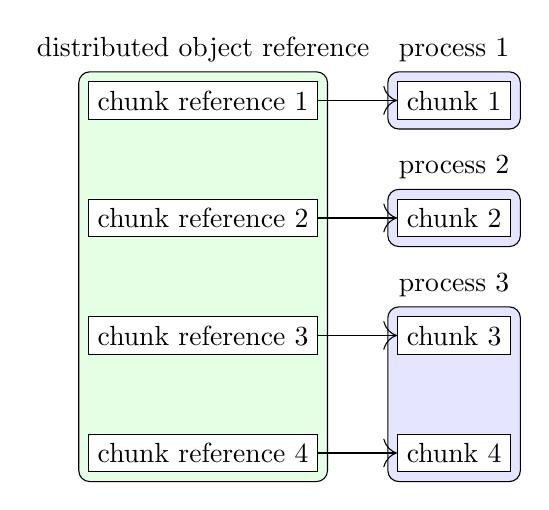
\begin{tikzpicture}
                \node[object] (cri) {chunk reference 1};
                \node[object,below=of cri] (crii) {chunk reference 2};
                \node[object,below=of crii] (criii) {chunk reference 3};
                \node[object,below=of criii] (criv) {chunk reference 4};

                \node[proc,right=of cri] (ci) {chunk 1};
                \node[proc,below=of ci] (cii) {chunk 2};
                \node[proc,below=of cii] (ciii) {chunk 3};
                \node[proc,below=of ciii] (civ) {chunk 4};

                \begin{pgfonlayer}{categories}
                        \node[category,fit=(cri)(crii)(criii)(criv),label={[name=distobjref]distributed object reference}] (dobj) {};
                \end{pgfonlayer}
                \begin{pgfonlayer}{units}
                        \node[unit,fit=(ci),label={process 1}] (p1) {};
                        \node[unit,fit=(cii),label={process 2}] (p2) {};
                        \node[unit,fit=(ciii)(civ),label={process 3}] (p3) {};
                \end{pgfonlayer}

                \draw[mypath] (cri) -- (ci);
                \draw[mypath] (crii) -- (cii);
                \draw[mypath] (criii) -- (ciii);
                \draw[mypath] (criv) -- (civ);
\end{tikzpicture}

\caption{\label{fig:top} Example distributed object reference relations}
\end{center}
\end{figure}

Communication structure is a further challenge, which has as its answer an implicit virtual topology of the distributed system.
\lsr engages distributed worker nodes in a peer-to-peer fashion, chunks being the core means of addressing, with their location made opaque at the user-level of the system.

Concurrency is an essential component to distributed systems, and this challenge saw its response as both in-process and inter-process concurrency with \lsr; the base supporting layer of the \lsr stack is a bespoke in-memory TCP message queue service that allows for communication between nodes concurrent with their other operations.
Between nodes, routines run asynchronously over chunks, with parallelism implicit and controlled in distributed fashion.

Evaluation and scope may serve to speciate languages, as in the case of \R from \proglang{S}, and they take special forms in a distributed system.
\lsr seeks to minimise any differences from the \R language, so as to provide as transparent an experience for developers as possible, but with respect to evaluation, differs in following a call-by-value, as opposed to call-by-need pattern. Furthermore, errors can be caught, but are only propogated to the caller upon emergence of the underlying chunks, with the system favouring asynchrony to strictness. Scope is likewise limited in favour of message transfer efficiency.

In order to enable complex and iterative models, a distributed garbage collection system is also essential.
Such a system should handle mutable underlying chunk data as well.
Mutable data is treated equivalently to immutable data, where all operations on chunks result in new references, with new identifiers, that are surjective to their referent chunks.
\texttt{largescaler} enables garbage collection in an efficient and conservative manner, through automatically keeping track of the directed acyclic graph of chunk generation history alongside each chunk reference, and clearing this upon proof of computation.
Chunks lacking references are marked for deletion and may then be removed by \texttt{R}'s internal garbage collection.

\section{Results}

\texttt{largescaler} serves as a functioning system, capable of performing complex statistical analyses over datasets spanning hundreds of nodes.
The implementation of this system makes use of a layered approach, wherein each layer targets a different category of user.
A description of the implementation structure of \texttt{largescaler} follows.

The system is supported at the base layer by the \texttt{orcv} package, which exists as an in-memory threaded TCP message queue.
It was created specifically for \texttt{largescaler}, making use of the \texttt{C} API for \texttt{R}, though it is sufficiently general to serve the wider purpose of a message queue for the transfer of \texttt{R} objects between \texttt{R} processes.
Central to the functionality of \texttt{orcv} is its multithreaded operation, allowing transfers to take place in the background of the host \texttt{R} process, thereby not blocking computation.
The core userbase of this package is intended as developers on \texttt{largescaler}.

Sitting on top of \texttt{orcv}, the package \texttt{chunknet} enables the creation of detached nodes, which use \texttt{orcv} to communicate, and operate using their own event loops populated via the queue provided by \texttt{orcv}.
The instances of these nodes provided by the package are worker nodes, and a location service, which serve to operate on and locate chunks, respectively.
The client interface is also provided by \texttt{chunknet}, allowing interaction with chunks as the major user-facing class in this package.
Chunks can be interacted with individually, or collected as part of arbitrary-dimension arrays, over which distributed \texttt{apply()}'s and the like are defined.
The main users of this package are intended to be power-users of distributed statistical algorithms who seek to maximise performance.

The package that meets the demanding statistician referenced in Section~\ref{sec:intro} is given by the \texttt{largescaler} package, which offers the distributed object as an abstracted class where chunk distribution is handled implicitly by the package, freeing the statistician to focus on model creation. Further features offered by the package include distributed environment setup, an automatic distributed function converter, distributed functional programming tools such as a reduce operator, distributed i/o, checkpointing, shuffling of datasets with implicit load-balancing, and a \texttt{dplyr} interface to distributed objects.

\section{Discussion}

The \texttt{largescaler} system has been proven over a number of application areas.
Data manipulation is a basic necessity, as it is required for modelling, and is provided well by other systems.
\texttt{largescaler} is capable of a full set of data manipulations, including all that are provided by the \texttt{dplyr} package.
Model fitting is demonstrated in the proof-of-concept \texttt{largescalemodelr} package, which includes a variety of models, including linear models and generalised linear models.
Work is currently underway to develop examples of boosted models, as well as a convex optimisation methods such as the alternating direction method of multipliers.

Initial benchmarking results are highly promising, with performance results measuring not only speed but capability;
One instance of capability is given in the creation of a contingency table of a large dataset that crashed \texttt{Spark} but was computed in several seconds using \texttt{largescaler}.

The scope for future work remains significant, enabled by the high level of extensibility provided by the system.
External systems which serve to monitor performance or take up the role of garbage collection would grant the possibility of greater reliabilit.
Robustness could be gained through self-healing datasets, a potential that has a precedent in a current prototype, which allows for resiliance to node failure in a more efficient manner than that of the current Resilient Distributed Datasets~\cite{zaharia2012resilient}.
Further resiliance can be gained within the system through operating the location service as a distributed hash table, leaving no central point of failure in a fully peer-to-peer system.


\chapter{Literature Review}
\hypertarget{introduction}{%
    \subsection{Introduction}\label{introduction}}

Statistics is concerned with the analysis of datasets, which are
continually growing bigger, and at a faster rate; the global datasphere
is expected to grow from 33 zettabytes in 2018 to 175 zettabytes by
2025\cite{rydning2018digitization}.

The scale of this growth is staggering, and continues to outpace
attempts to engage meaningfully with such large datasets. By one
measure, information storage capacity has grown at a compound annual
rate of 23\% per capita over recent decades\cite{hilbert2011world}. In
spite of such massive growths in storage capacity, they are far
outstripped by computational capacity over time \cite{fontana2018moore}.
Specifically, the number of components comprising an integrated circuit
for computer processing have been exponentially increasing, with an
additional exponential decrease in their cost\cite{moore1975progress}.
This observation, known as Moore's Law, has been the root cause for much
of computational advancement over the past half-century. The
corresponding law for computer storage posits increase in bit density of
storage media along with corresponding decreases in price, which has
been found to track lower than expected by Moore's law metrics. Such
differentials, between the generation of data, computational capacity
for data processing, and constraints on data storage, have forced new
techniques in computing for the analysis of large-scale data.

The architecture of a computer further constrains the required approach
for analysis of big data. Most general-purpose PC's are modelled by a
random-access stored-program machine, wherein a program and data are
stored in registers, and data must move in and out of registers to a
processing element, most commonly a Central Processing Unit (CPU). The
movement takes at least one cycle of a computer's clock, thereby leading
to larger processing time for larger data.

Reality dictates many different forms of data storage, with a Memory
Hierarchy ranking different forms of computer storage based on their
response times\cite{toy1986computer}. The volatility of memory (whether
or not it persists with no power) and the expense of faster storage
forms dictates the design of commodity computers. An example of a
standard build is given by the Dell Optiplex 5080, with 16Gb of Random
Access Memory (RAM) for fast main memory, to be used as a program data
store; and a 256Gb Solid State Drive (SSD) for slow long-term disk
storage\cite{cornell2021standardcomp}. For reasonable speed when
accessing data, a program would prioritise main memory over disk storage
- something not always possible when dataset size exceeds memory
capacity, larger-than-memory datasets being a central issue in big data.
A program that is primarily slowed by data movement is described as
I/O-bound, or memory-bound. Much of the issue in modelling large data is
the I/O-bound nature of much statistical computation.

The complement to I/O-bound computation is computation-bound,
wherein the speed (or lack thereof) is determined primarily through the
performance of the processing unit. This is less significant in
large-scale applications than memory-bound, but remains an important
design consideration when the number of computations scale with the
dataset size in any nontrivial algorithm with greater than
\(\mathcal{O}(1)\) complexity.

The solution to both memory- and computation-bound problems has largely
been that of using more hardware; more memory, and more CPU cores. Even
with this in place, more complex software is required to manage the more
complex systems. As an example, with additional CPU cores, constructs
such as multithreading are used to perform processing across multiple
CPU cores simultaneously (in parallel).

The means for writing software for large-scale data is typically through
the use of a structured, high-level programming language. Of the myriad
programming languages, the most widespread language used for statistics
is R. As of 2021, R increased in popularity to rank 9th in the TIOBE
index. R also has a special relevance for this proposal, having been
initially developed at the University of Auckland by Ross Ihaka and
Robert Gentleman in 1991\cite{ihaka1996r}.

Major developments in contemporary statistical computing are typically
published alongside R code implementation, usually in the form of an R
package, which is a mechanism for extending R and sharing functions. As
of March 2021, the Comprehensive R Archive Network (CRAN) hosts over
17000 available packages\cite{team20:_r}. Several of these packages are
oriented towards managing large datasets, and will be assessed in
\ref{sec:local}\ref{sec:dist} below. This project aims to develop an R
package that provides a means for writing software to analyse very large
data on clusters consisting of multiple general-purpose computers.
\section{Strategies for Handling Large Scale Data}
\hypertarget{sec:parallel}{%
	\subsection{Parallelism as a Strategy}\label{sec:parallel}}

The central strategy for manipulating large datasets, from which most
other patterns derive, is parallelisation. To parallelise is to engage
in many computations simultaneously - this typically takes the form of
either task parallelism, wherein tasks are distributed across different
processors; data parallelism, where the same task operates on different
pieces of data across different processors; or some mix of the two.

Parallelisation of a computational process can potentially offer
speedups proportional to the number of processors available to take on
work, and with recent improvements in multiprocessor hardware, the
number of processors available is increasing over time. Most
general-purpose personal computers produced in the past 5 years have
multiple processor cores to enable parallel computation.

Parallelism can afford major speedups, albeit with certain limitations.
Amdahl's law, formulated in 1967, aims to capture the speedup
limitations, with a model derived from the argument given below in
\ref{eq:amdahlsform}\cite{amdahl1967law}\cite{gustafson1988law}:

\begin{equation*}\label{eq:amdahlsform}
	\textrm{Speedup} = \frac{1}{s+\frac{p}{N}}
\end{equation*}

Where,

\begin{description}
	\item[Speedup] total speedup of whole task
	\item[s] time spend by serial processor on inherently serial part of program
	\item[p] time spent by serial processor on parallelisable part of program
	\item[N] number of processors
\end{description}

The implication is that speedup of an entire task when parallelised is
granted only through the portion of the task that is otherwise
constrained by singular system resources, at the proportion of execution
time spent in that task. Thus a measure of skepticism is contained in
Amdahl's argument, with many tasks predicted to show no benefit to
parallelise - and in reality, some likely to slow down with increased
overhead given in parallelisation.

The major response to the skepticism of Amdahl's law is given by
Gustafson's law, generated from timing results in a highly parallelised
system. Gustafson's law presents a scaled speedup as per
\ref{eq:gustafsonsform}

\begin{equation}\label{eq:gustafsonsform}
	\textrm{Scaled speedup} = s' + p'N = N + (1-N)s'
\end{equation}

Where,

\begin{description}
	\item[s'] serial time spent on the parallel system
	\item[p'] parallel time spent on the parallel system
\end{description}

This law implies far higher potential parallel speedup, varying linearly
with the number of processors.

An example of an ideal task for parallelisation is the category of
embarassingly parallel workload. Such a problem is one where the
separation into parallel tasks is trivial, such as performing the same
operation over a dataset independently\cite{foster1995parallel}. Many
problems in statistics fall into this category, such as tabulation,
monte-carlo simulation and many matrix manipulation tasks.

\hypertarget{sec:local}{%
	\subsection{Local Solutions}\label{sec:local}}

While not specifically engaging with larger-than-memory data, a number
of packages take advantage of various parallel strategies in order to
process large datasets efficiently. \textbf{multicore} is one such
package, now subsumed into the \textbf{parallel} package, that grants
functions that can make direct use of multiprocessor systems, thereby
reducing the processing time in proportionality to the number of
processors available on the system.

\textbf{data.table} also makes use of multi-processor systems, with many
operations involving threading in order to rapidly perform operations on
its dataframe equivalent, the data.table.

In spite of all of these potential solutions, a major constraint remains
in that only a single machine is used. As long as there is only one
machine available, bottlenecks form and no redundancy protection is
offered in real-time in the event of a crash or power outage.

The first steps typically taken to manage larger-than-memory data is to
shift part of the data into secondary storage, which generally possesses
significantly more space than main memory.

This is the approach taken by the \textbf{disk.frame} package, developed
by Dai ZJ. \textbf{disk.frame} provides an eponymously named dataframe
replacement class, which is able to represent a dataset far larger than
RAM, constrained now only by disk size\cite{zj20}.

The mechanism of disk.frame is introduced on its homepage with the
following explanation:

\begin{displayquote}
	\{disk.frame\} works by breaking large datasets into smaller individual
	chunks and storing the chunks in fst files inside a folder. Each chunk
	is a fst file containing a data.frame/data.table. One can construct the
	original large dataset by loading all the chunks into RAM and row-bind
	all the chunks into one large data.frame. Of course, in practice this
	isn't always possible; hence why we store them as smaller individual
	chunks. \{disk.frame\} makes it easy to manipulate the underlying chunks
	by implementing dplyr functions/verbs and other convenient functions
	(e.g.~the \mintinline{r}{cmap(a.disk.frame, fn, lazy = F)}
	function which applies the function fn to each chunk of a.disk.frame in
	parallel). So that \{disk.frame\} can be manipulated in a similar
	fashion to in-memory data.frames.
\end{displayquote}

It works through two main principles: chunking, and an array of methods
taking advantage of data.frame generics, including \textbf{dplyr} and
\textbf{data.table} functions.

Another component that isn't mentioned in the explanation, but is
crucial to performance, is the parallelisation offered transparently by
the package.

disk.frames are actually references to numbered \mintinline{r}{fst} files in a
folder, with each file serving as a chunk.
This is made use of through manipulation of each chunk separately,
sparing RAM from dealing with a single monolithic
file\cite{zj19:_inges_data}.
Fst is a means of serialising dataframes, as an alternative to RDS
files\cite{klik19}.
It makes use of an extremely fast compression algorithm developed at
facebook.
Functions are usually mapped over chunks using some functional, but more
complex functions such as those implementing a glm require custom
solutions; as an example the direct modelling function of
\mintinline{r}{dfglm()} is implemented to allow
for fitting glms to the data.
From inspection of the source code, the function is a utility wrapper
for streaming disk.frame data by default into bigglm, a biglm
derivative.
For grouped or aggregated functions, there is more complexity involved,
due to the chunked nature of disk.frame.
When functions are applied, they are by default applied to each chunk.
If groups don't correspond injectively to chunks, then the syntactic
chunk-wise summaries and their derivatives may not correspond to the
semantic group-wise summaries expected.
For example, summarising the median is performed by using a
median-of-medians method; finding the overall median of all chunks'
respective medians.

Therefore, computing grouped medians in disk.frame result in estimates
only --- this is also true of other software, such as spark, as noted in
\cite{zj19:_group_by}.
For parallelisation, future is used as the backend package, with most
function mappings on chunks making use of
\mintinline{r}{future::future_lapply()}
to have each chunk mapped with the intended function in parallel.
future is initialised with access to cores through the wrapper function,
\mintinline{r}{setup_disk.frame()}\cite{zj19:_key}.
This sets up the correct number of workers, with the minimum of workers
and chunks being processed in parallel.
An important aspect to parallelisation through future is that, for
purposes of cross-platform compatibility, new R processes are started
for each worker\cite{zj19:_using}.
Each process will possess its own environment, and disk.frame makes use
of future's detection capabilities to capture external variables
referred to in calls, and send them to each worker.
The strategy taken by \textbf{disk.frame} has several inherent
limitations, however. \textbf{disk.frame} allows only embarassingly
parallel operations for custom operations as part of a
split-apply-combine (MapReduce) pattern.
While there may theoretically be future provision for non-embarrassingly
parallel operations, a significant limitation to real-time operation is
the massive slowdown brought by the data movement from disk to RAM and
back.

\hypertarget{sec:dist}{%
	\section{Distributed Computing as a Strategy}\label{sec:dist}}

The specs of a single contemporary commodity computer are higher than
those that were used in the Apollo lunar landing, yet the management of
large datasets still creates major issues, driven by a simple lack of
capacity to hold them in memory. Supercomputers can surmount this by
holding orders of magnitude higher memory, though only a few
organisations or individuals can bear the financial costs of purchasing
and maintaining a supercomputer.

In a similar form, cloud computing is not a universal solution, owing to
expense, security issues, and data transportation problems. Despite
this, systems rivalling supercomputers can be formed through combining
many commodity computers. An amusing illustration of this was given in
2004, when a flash mob connected hundreds of laptops to attempt running
the linpack benchmark, achieving 180 gigaflops in processing
output\cite{perry2004flashcomp}.

The combination of multiple independent computers to form one cohesive
computing system forms part of what is known as distributed computing.
More serious efforts to connect multiple commodity computers into a
larger computational system is now standard, with software such as
Hadoop and Spark being commonplace in large companies for the purpose of
creating distributed systems.

Distributed systems make possible the real-time manipulation of datasets
larger than a single computer's RAM, by splitting up data and holding it
in the RAM of multiple computers. A factor strongly serving in favour of
distributed computing is that commodity hardware exists in large
quantities in most offices, oftentimes completely unused. This means
that many organisations already have the necessary base infrastructure
to create a distributed system, likely only requiring some software and
configuration to set it all up. Beyond the benefit of pre-existing
infrastructure, a major feature commonly offered by distributed systems,
and lacking in high-powered single computer systems, is that of fault
tolerance - when one computer goes down, as does happen, another
computer in the system had redundant copies of much of the information
of the crashed computer, and computation can resume with very little
inconvenience. A single computer, even very high-powered, doesn't
usually offer fault-tolerance to this degree.

All of the packages examined the above \ref{sec:local} have no
immediate capability to create a distributed system, and have all of the
ease-of-use benefits and all of the drawbacks as discussed.

\hypertarget{distributed-large-scale-computing}{%
	\section{Distributed Large-Scale Computing}\label{distributed-large-scale-computing}}

R does have some well-established packages used for distributed
large-scale computing. Of these, the \textbf{parallel} package is
contained in the standard R image, and encapsulates \textbf{SNOW}
(Simple Network Of Workstations), which provides support for distributed
computing over a simple network of compputers. The general architecture
of \textbf{SNOW} makes use of a master process that holds the data and
launches the cluster, pushing the data to worker processes that operate
upon it and return the results to the master. \textbf{SNOW} makes use of
several different communications mechanisms, including sockets or the
greater MPI distributed computing library. Some shortcomings of the
described architecture is the difficulty of persisting data, meaning the
expense of data transportation every time operations are requested by
the master process. In addition, as the data must originate from the
master (barring generated data etc.), the master's memory size serves as
a bottleneck for the whole system.

The \textbf{pbdR} (programming with big data in R) project provides
persistent data, with the \textbf{pbdDMAT} (programming with big data
Distributed MATrices) package offering a user-friendly distributed
matrix class to program with over a distributed system. It is introduced
on its main page with the following description:

\begin{displayquote}
	The ``Programming with Big Data in R'' project (pbdR) is a set of highly
	scalable R packages for distributed computing and profiling in data
	science. Our packages include high performance, high-level interfaces to
	MPI, ZeroMQ, ScaLAPACK, NetCDF4, PAPI, and more. While these libraries
	shine brightest on large distributed systems, they also work rather well
	on small clusters and usually, surprisingly, even on a laptop with only
	two cores. Winner of the Oak Ridge National Laboratory 2016 Significant
	Event Award for ``Harnessing HPC Capability at OLCF with the R Language
	for Deep Data Science.'' OLCF is the Oak Ridge Leadership Computing
	Facility, which currently includes Summit, the most powerful computer
	system in the world.
\end{displayquote}\cite{pbdR2012}

The project seeks especially to serve minimal wrappers around the BLAS
and LAPACK libraries along with their distributed derivatives, with the
intention of introducing as little overhead as possible. Standard R also
uses routines from the library for most matrix operations, but suffers
from numerous inefficiencies relating to the structure of the language;
for example, copies of all objects being manipulated will be typically
be created, often having devastating performance aspects unless specific
functions are used for linear algebra operations, as discussed in
\cite{schmidt2017programming} (e.g.,
\mintinline{r}{crossprod(X)} instead of \mintinline{r}{t(X) %*% X})

Distributed linear algebra operations in pbdR depend further on the
ScaLAPACK library, which can be provided through the pbdSLAP package
\cite{Chen2012pbdSLAPpackage}. The principal interface for direct
distributed computations is the pbdMPI package, which presents a
simplified API to MPI through R \cite{Chen2012pbdMPIpackage}. All major
MPI libraries are supported, but the project tends to make use of
openMPI in explanatory documentation. A very important consideration
that isn't immediately clear is that pbdMPI can only be used in batch
mode through MPI, rather than any interactive option as in Rmpi
\cite{yu02:_rmpi}.

The actual manipulation of distributed matrices is enabled through the
pbdDMAT package, which offers S4 classes encapsulating distributed
matrices \cite{pbdDMATpackage}. These are specialised for dense matrices
through the \mintinline{r}{ddmatrix} class, though the project offers some
support for other matrices. The \mintinline{r}{ddmatrix} class has nearly all
of the standard matrix generics implemented for it, with nearly
identical syntax for all.

The package is geared heavily towards matrix operations in a statistical
programming language, so a test of its capabilities would quite
reasonably involve statistical linear algebra. An example non-trivial
routine is that of generating data, to test randomisation capability,
then fitting a generalised linear model to the data through iteratively
reweighted least squares. In this way, not only are the basic algebraic
qualities considered, but communication over iteration on distributed
objects is tested.

To work comparatively, a simple working local-only version of the
algorithm is produced in listing \ref{lst:local-rwls}.

\begin{listing}
	\begin{minted}{r}
set.seed(1234)
# Generate the data

n <- 1000
B <- matrix(c(1,3))
x0 <- rep(1, n)
x1 <- rnorm(n, 0, 1)
X <- cbind(x0, x1)
p <- 1 / (1 + exp(- X %*% B))
y <- rbinom(n, 1, p)

# Base comparison
#glm(y ~ x1, family = "binomial")

# RWLS as Newton-Raphson for GLM (logistic regression here)

logReg <- function(X, y, maxIter=80, tolerance=0.01){
	pr <- function(X, B){
		1 / (1 + exp(-X  %*% B))
	}
	##
	weights <- function(X, B, y){
		diag(as.vector(pr(X, B)))
	}
	##
	oldB <- matrix(c(Inf,Inf))
	newB <- matrix(c(0, 0))
	nIter <- 0
	while (colSums((newB - oldB)^2) > tolerance &&
	       nIter < maxIter) {
		oldB <- newB
	## N-R as RWLS
		W <- weights(X, oldB, y)
		hessian <- - t(X) %*% W %*% X
		z <- X %*% oldB + solve(W) %*% (y - pr(X, oldB))
		newB <- solve(-hessian) %*% crossprod(X, W %*% z)
	##
		nIter <- nIter + 1
	}
	newB
}

print(logReg(X, y, tolerance=1E-6, maxIter=100))
\end{minted}
	\caption{Local GLM with RWLS}
	\label{lst:local-rwls}
\end{listing}

It outputs a \(\hat{\beta}\) matrix after several seconds of
computation.

Were pbdDMAT matrices to function perfectly transparently as regular
matrices, then all that would be required to convert a local algorithm
to distributed would be to prefix a \mintinline{r}{dd} to every \mintinline{r}{matrix}
call, and bracket the program with a template as per listing
\ref{lst:bracket}.

\begin{listing}
	\begin{minted}{r}
suppressMessages(library(pbdDMAT))
init.grid()

# program code with `dd` prefixed to every `matrix` call

finalize()
\end{minted}
	\caption{Idealised Common Wrap for Local to Distributed Matrices}
	\label{lst:bracket}
\end{listing}

The program halts however, as forms of matrix creation other than
through explicit \mintinline{r}{matrix()} calls
are not necessarily picked up by that process; \mintinline{r}{cbind} requires a
second formation of a \mintinline{r}{ddmatrix}.

The first issue comes when performing conditional evaluation; predicates
involving distributed matrices are themselves distributed matrices, and
can't be mixed in logical evaluation with local predicates.

Turning local predicates to distributed matrices, then converting them
all back to a local matrix for the loop to understand, finally results
in a program run, however the results are still not accurate.

This is due to
\mintinline{r}{diag()<-}
assignment not having been implemented, so several further changes are
necessary, including specifying return type of the diag matrix as a
replacement.

This serves to outline the difficulty of complete distributed
transparency.

The final working code of pbdDMAT GLM through RWLS is given in listing
\ref{lst:dmat}

\begin{listing}
	\begin{minted}{r}

suppressMessages(library(pbdDMAT))
init.grid()

set.seed(1234)
# Generate the data

n <- 1000
B <- ddmatrix(c(1,3))
x0 <- rep(1, n)
x1 <- rnorm(n, 0, 1)
X <- as.ddmatrix(cbind(x0, x1))
p <- 1 / (1 + exp(- X %*% B))
y <- ddmatrix(rbinom(n, 1, as.vector(p)))

# Base comparison
#glm(y ~ x1, family = "binomial")

# RWLS as Newton-Raphson for GLM (logistic regression here)

logReg <- function(X, y, maxIter=80, tolerance=0.01){
	pr <- function(X, B){
		1 / (1 + exp(-X  %*% B))
	}
	##
	weights <- function(X, B, y){
		diag(as.vector(pr(X, B)), type="ddmatrix")
	}
	##
	oldB <- ddmatrix(c(Inf,Inf))
	newB <- ddmatrix(c(0, 0))
	nIter <- ddmatrix(0)
	maxIter <- as.ddmatrix(maxIter)
	while (as.matrix(colSums((newB - oldB)^2) > tolerance &
	       nIter < maxIter)) {
		oldB <- newB
	## N-R as RWLS
		W <- weights(X, oldB, y)
		hessian <- - t(X) %*% W %*% X
		z <- X %*% oldB + solve(W) %*% (y - pr(X, oldB))
		newB <- solve(-hessian) %*% crossprod(X, W %*% z)
	##
		nIter <- nIter + 1
	}
	newB
}

print(logReg(X, y, tolerance=1E-6, maxIter=100))

finalize()
\end{minted}
	\caption{pbdDMAT GLM with RWLS}
	\label{lst:dmat}
\end{listing}

Decidedly more user-friendly is the \textbf{sparklyr} package, which
meshes \textbf{dplyr} syntax with a \textbf{Spark} backend. Simple
analyses are made very simple (assuming a well-configured and already
running \textbf{Spark} instance), but custom iterative models are
extremely difficult to create through the package in spite of
\textbf{Spark's} support for it.

Given that iteration is cited by a principal author of Spark as a
motivating factor in its development when compared to Hadoop, it is
reasonable to consider whether the most popular R interface to Spark,
sparklyr, has support for
iteration\cite{zaharia2010spark}\cite{luraschi20}. One immediate
hesitation to the suitability of sparklyr to iteration is the syntactic
rooting in dplyr; dplyr is a ``Grammar of Data Manipulation'' and part
of the tidyverse, which in turn is an ecosystem of packages with a
shared philosophy\cite{wickham2019welcome}\cite{wickham2016r}. The
promoted paradigm is functional in nature, with iteration using for
loops in R being described as ``not as important'' as in other
languages; map functions from the tidyverse purrr package are instead
promoted as providing greater abstraction and taking much less time to
solve iteration problems. Maps do provide a simple abstraction for
function application over elements in a collection, similar to internal
iterators, however they offer no control over the form of traversal, and
most importantly, lack mutable state between iterations that standard
loops or generators allow\cite{cousineau1998functional}.

A common functional strategy for handling a changing state is to make
use of recursion, with tail-recursive functions specifically referred to
as a form of iteration in \cite{abelson1996structure}. Reliance on
recursion for iteration is naively non-optimal in R however, as it lacks
tail-call elimination and call stack optimisations\cite{rcore2020lang};
at present the elements for efficient, idiomatic functional iteration
are not present in R, given that it is not as functional a language as
the tidyverse philosophy considers it to be, and sparklyr's attachment
to the the ecosystem prevents a cohesive model of iteration until said
elements are in place.

Iteration takes place in Spark through caching results in memory,
allowing faster access speed and decreased data movement than
MapReduce\cite{zaharia2010spark}. sparklyr can use this functionality
through the \mintinline{r}{tbl_cache()} function to
cache Spark dataframes in memory, as well as caching upon import with
\mintinline{r}{memory=TRUE} as a formal parameter to
\mintinline{r}{sdf_copy_to()}. Iteration can also
make use of persisting Spark Dataframes to memory, forcing evaluation
then caching; performed in sparklyr through
\mintinline{r}{sdf_persist()}.

An important aspect of consideration is that sparklyr methods for dplyr
generics execute through a translation of the formal parameters to Spark
SQL. This is particularly relevant in that separate Spark Data Frames
can't be accessed together as in a multivariable function. In addition,
very R-specific functions such as those from the \textbf{stats} and
\textbf{matrix} core libraries are not able to be evaluated, as there is
no Spark SQL cognate for them.

Canned models are the only option for most users, due to
\textbf{sparklyr's} reliance on Spark SQL rather than the Spark core API
made available through the official \textbf{SparkR} interface.

sparklyr is excellent when used for what it is designed for. Iteration,
in the form of an iterated function, does not appear to be part of this
design.

Furthermore, all references to ``iteration'' in the primary sparklyr
literature refer either to the iteration inherent in the inbuilt Spark
ML functions, or the ``wrangle-visualise-model'' process popularised by
Hadley Wickham\cite{luraschi2019mastering}\cite{wickham2016r}. None of such
references connect with iterated functions.

\hypertarget{other-systems}{%
	\subsection{Other Systems}\label{other-systems}}

In the search for a distributed system for statistics, the world outside
of R is not entirely barren. The central issue with non-R distributed
systems is that their focus is very obviously not statistics, and this
shows in the level of support the platforms provide for statistical
purposes.

The classical distributed system for high-performance computing is MPI.
R actually has a high-level interface to MPI through the \textbf{rmpi}
package. This package is excellent, but extremely low-level, offering
little more than wrappers around MPI functions. For the statistician who
just wants to implement a model for a large dataset, such concern with
minutiae is prohibitive.

Hadoop and Spark are two closely related systems which were mentioned
earlier.

Apache Hadoop is a collection of utilities that facilitates cluster
computing.

Jobs can be sent for parallel processing on the cluster directly to the
utilities using .jar files, ``streamed'' using any executable file, or
accessed through language-specific APIs.

The project began in 2006, by Doug Cutting, a Yahoo employee, and Mike
Cafarella.

The inspiration for the project was a paper from Google describing the
Google File System (described in \cite{ghemawat2003google}), which was
followed by another Google paper detailing the MapReduce programming
model, \cite{dean2004mapreduce}.

Hadoop consists of a file-store component, known as Hadoop Distributed
File System (HDFS), and a processing component, known as MapReduce.

In operation, Hadoop splits files into blocks, then distributes them
across nodes in a cluster (HDFS), where they are then processed by the
node in parallel (MapReduce). This creates the advantage of data
locality, wherein data is processed by the node they exist in.

Hadoop has seen extensive industrial use as the premier big data
platform upon its release.

In recent years it has been overshadowed by Spark, due to the greater
speed gains offered by Spark for many problem sets.

Spark was developed with the shortcomings of Hadoop in mind; Much of
its definition is in relation to Hadoop, which it intended to improve
upon in terms of speed and usability for certain
tasks\cite{zaharia2010spark}.

its fundamental operating concept is the Resiliant Distributed Dataset
(RDD), which is immutable, and generated through external data, as well
as actions and transformations on prior RDD's.

The RDD interface is exposed through an API in various languages,
including R, however it appears to be abandoned to some degree, having
removed from the CRAN repository at 2020-07-10 due to failing checks.

Spark requires a distributed storage system, as well as a cluster
manager; both can be provided by Hadoop, among others.

Spark is known for possessing a fairly user-friendly API, intended to
improve upon the MapReduce interface.

Another major selling point for Spark is the libraries available that
have pre-made functions for RDD's, including many iterative algorithms.

The availability of broadcast variables and accumulators allow for
custom iterative programming.

Spark has seen major use since its introduction, with effectively all
major big data companies having some use of Spark.

In the python world, the closest match to a high-level distributed
system that could have statistical application is given by the python
library \textbf{dask}\cite{rocklin2015dask}. \textbf{dask} offers
dynamic task scheduling through a central task graph, as well as a set
of classes that encapsulate standard data manipulation structures such
as NumPy arrays and Pandas dataframes.

The main difference is that the \textbf{dask} classes take advantage of
the task scheduling, including online persistence across multiple nodes.
\textbf{dask} is a large and mature library, catering to many use-cases,
and exists largely in the Pythonic ``Machine Learning'' culture in
comparison to the R ``Statistics'' culture. Accordingly, the focus is
more tuned to the Python software developer putting existing ML models
into a large-scale capacity. Of all the distributed systems assessed so
far, \textbf{dask} comes the closest to what an ideal platform would
look like for a statistician, but it misses out on the statistical
ecosystem of R, provides only a few select classes, and is tied entirely
to the structure of the task graph.

\section{Common Features of Large Scale Data Platforms}
\hypertarget{a-survey-of-large-scale-platform-features}{%
  \section{A Survey of Large-Scale Platform
    Features}\label{a-survey-of-large-scale-platform-features}}

\hypertarget{sec:intro}{%
  \subsection{Introduction}\label{sec:intro}}

To guide the development of the platform, desirable features are drawn
from existing platforms; inferred as logical extensions; and arrived at
through identification of needs. Some features are mutually exclusive,
others are suggestive of each other, but are worth considering and
contrasting their merits.

\hypertarget{sec:feature-list}{%
  \subsection{Feature List}\label{sec:feature-list}}

A list of features and their descriptions follows:

\begin{description}
  \item[Distributed Computation]
    The ability to spread computation and data over separate computers. The
    value of distributed computing is well recognised for large-scale
    computing, in the increased capacity for processing, memory, and
    storage. Distributed computing typically gains latency speedup through
    parallel processing; both Amdahl's law and Gustafson's law give
    theoretical speedups for parallel jobs \cite{amdahl1967law}
    \cite{gustafson1988law}. In addition, each node typically adds more working
    memory to the distributed system, allowing for larger datasets to be
    manipulated in-memory. For exceedingly large datasets, the benefits of
    distributed file systems commonly allow for resiliant storage, with
    well-regarded examples including HDFS and the Google File System it is
    based upon \cite{shvachko2010hadoop}\cite{ghemawat2003google}.
  \item[Evaluation of User-Specified Code]
    The ability to make use of user-specified code in processing. Most R
    packages for large-scale computing interact well with arbitrary code,
    however they typically have some limitations, such as an inability to
    recognise global variables, as is the case with sparklyr and to a lesser
    extent future \cite{sparklyr2020limitations}\cite{microsoft20}.
  \item[Native Support for Iteration]
    The ability to process user-specified code involving iteration over the
    whole dataset natively, keeping results in memory between iterations.
    This reflects the inherently iterative nature of many statistical
    algorithms. Furthermore, this shouldn't initiate a new job or process
    for every new iteration. This is seen as important enough that it serves
    as a major motivating factor behind Spark's development, overcoming a
    perceived major deficiency of Hadoop by Spark's developers
    \cite{zaharia2010spark}.
  \item[Object Persistence at Nodes]
    The ability to retain objects in-memory at their point of processing.
    The standard motivation for such a feature revolves around a reduction
    in data movement, which serves to slow down processing enormously
    through forcing programs to be I/O bound. In-memory persistence is
    closely related to the capacity for iterative code evaluation in a
    distributed system, and was similarly referenced by the Spark developers
    as an apparent benefit of Spark\cite{zaharia2010spark}.
  \item[Support for Distributed File Systems]
    Capacity to work with data and computation on distributed file systems,
    with a particular target of Hadoop Distributed File System (HDFS). As a
    well-established distributed file system, HDFS is targeted by a number
    of R packages, as well as serving as a file system base for other
    platforms such as spark \cite{analytics:_rhadoop_wiki}
    \cite{deltarho:_rhipe}\cite{urbanek20}\cite{zaharia2016apache}. HDFS offers
    several features that make it particularly attractive as a filesystem
    for a large-scale statistical analysis; being distributed and capable of
    running on commodity hardware allows for truly big data analysis. In
    addition, the system is built to be resiliant to hardware failure, so
    long-running analyses aren't cut short or forced to revert to a
    checkpoint because of singular component failure
    \cite{shvachko2010hadoop}.
  \item[Ease of Setup]
    Is setup suitable for a computationally-focussed statistician, or does
    it require a system administrator? At it's base, R is a statistical
    programming language \cite{rcore2020intro}. The particular skills of
    statisticians seldom correspond to the those requisite of system
    administration, with such a focus unlikely to compete successfully with
    their main research. Ease of deployment can determine a platform's
    success, with such a feature being one of the many motivations for the
    use and development of tools such as docker in recent years. The easiest
    possible setup would be a regular
    \mintinline{r}{install.packages()}, with no more than
    several lines specifying the platform configuration.
  \item[Inter-Node Communication]
    Can any pair of nodes communicate with each other, or do they only
    report to a master node? While many tasks process efficiently within a
    standard master-slave architecture, and inter-node communication is
    inherently expensive, there is still a large class of tasks that benefit
    from inter-node communication\cite{walker1996mpi}; particularly
    graph-based statistical methods.
  \item[Interactive Usage]
    The ability to make use of the package in an interactive R session,
    without mandatory batch execution. A major benefit of R as being
    interpreted is the availability of the REPL. The benefits of
    interactivity stemming from a REPL are well-documented, most notably
    aiding debugging \cite{mccarthy1978history}. For statistical analysese
    in particular, interactive analyses play a major role in exploratory
    data analysis, wherein insights can be tested and arrived at rapidly
    with an interactive session.
  \item[Backend Decoupling]
    The implementation is maintained entirely separately to the interface.
    This is standard in most of the performant parallel R systems as
    described by \cite{eddelbuettel2019parallel}, including foreach as a key
    example\cite{microsoft20}. As a software pattern, this is a case of
    separation of concerns, described in detail by \cite{dijkstra1982role}.
    Such a pattern fosters modularity and allows for a broader range of
    backends to be made use of, maximising the uptake of the platform. The
    ability for a system to adhere to a similar interface despite changes in
    internal behaviour is additionally useful for the sake of referential
    transparency, which prevents the need to rewrite programs upon making
    changes, as well as for human-computer interaction considerations
    \cite{sondergaard1990Rtda}\cite{norman2013design}. For example, the foreach
    package can change parallel adaptors in a single line of setup, without
    needing any changes made in the code referencing future, despite making
    use of a different internal interface \cite{weston19:_using}.
  \item[Evaluation of Arbitrary Classes]
    Any class, including user-defined classes, can be used in evaluation.
    There is proven value in rich user-defined objects, with the weight of
    much of the object-oriented programming paradigm serving to further that
    point \cite{dahl2004simula}. Conversely, many major packages limit
    themselves through provisioning only a few classes, such as pbdDMAT with
    distributed matrices, or the tidyverse and it's derivatives including
    sparklyr with ``tibbles'' \cite{pbdDMATpackage}\cite{wickham2019welcome}
  \item[Package-specific API]
    The platform is primarily explicitly programmed against at a
    package-specific interface. This is in contrast to packages mostly
    providing methods which overload standard generics or language
    structure; at a loss of general transparency, direct API's can ensure
    greater encapsulation and a closer mapping of code with the underlying
    implementation, thus potentially resulting in performance gains
    \cite{bierhoff2009api}. An example in R is the interface to the foreach
    package not overloading the existing for-loop syntax in R, but defining
    it's own specific interface \cite{microsoft20}.
  \item[Methods for Standard Generics]
    The platform is primarily programmed against using a polymorphic
    interface, with the package methods taking advantage of common generics.
    pbdDMAT takes this approach, as well as bigmemory, in providing
    matrix-like classes which are operated upon using standard matrix
    generics \cite{pbdDMATpackage}\cite{kane13:bigmemory}.
  \item[Methods for dplyr Generics]
    The platform makes use of dplyr functions as the primary set of generics
    to program over. Using a dplyr interface is a common trend in several R
    packages including sparklyr, disk.frame, and many database interfaces
    \cite{luraschi20}\cite{zj20}. Such an interface is claimed by the dplyr
    creators to aid beginners through being simple to remember
    \cite{wickham2019welcome}. In this way, it may serve to ease the
    learning curve for the platform.
\end{description}

\hypertarget{sec:comp-tab}{%
  \subsection{Comparison Table}\label{sec:comp-tab}}

\begin{table}[htbp]
  \centering\begin{tabular}{llllll}
    \toprule
    Feature                                                              & RHadoop                                                               & sparklyr                                      & pbdR                                        & disk.frame & foreach \\
    \midrule
    Distributed Computation                                              & yes\footnote{Use of HDFS through
      rhdfs\cite{revo2013rhdfs}, and MapReduce through
    rmr2\cite{revo2014plyrmr}}                                           & yes\footnote{Use of
    Spark\cite{luraschi20}}                                              & yes\footnote{Distributed computation
      performed by pbdMPI, with support for several remote messaging
    protocols\cite{Chen2012pbdMPIpackage}\cite{Schmidt2015pbdCSpackage}} & no
                                                                         & yes\footnote{Through the use of additional packages such as doMPI and
    sparklyr\cite{weston17}\cite{luraschi20}}                                                                                                                                                                                                                         \\
    Evaluation of User-Specified Code                                    & yes\footnote{rmr2\cite{revo2015rmr2}
    allows for arbitrary R code to be executed through MapReduce}        &
    mostly\footnote{Provides \mintinline{r}{mutate()}
      function to enable user-defined code, however there are limitations in
    not being capable of parsing global variables}                       & mostly\footnote{Adhering
    to a SPMD paradigm}                                                  & some\footnote{Many functions used for grouped
      summarisation are only estimates, such as
    \mintinline{r}{median}\cite{zj19:_group_by}}                         & mostly\footnote{\mintinline{r}{\%dopar\%}
      accepts any expression, and tries its best to handle references to
      global variables, however it is still recommended to manually define
    the global references as well as packages used}                                                                                                                                                                                                                   \\
    Native Support for Iteration                                         & no                                                                    & no\footnote{See
    doc/review-sparklyr-iteration.tex}                                   & yes                                                                   & no{3x4}                                       &
    no\footnote{foreach makes use of iterators, which can be defined to
      perform recurrance relations (see doc/review-foreach.tex, subsection
      ``Form of Iteration'') but these rely on closures and may in fact be
    slower than serial relations}                                                                                                                                                                                                                                     \\
    Object Persistence at Nodes                                          & no                                                                    & yes\footnote{See {2x3}}                       & yes
                                                                         & NA                                                                    & no                                                                                                                 \\
    Support for Distributed File Systems                                 & yes\footnote{Direct access to
    HDFS through rhdfs\cite{revo2013rhdfs}}                              & yes\footnote{Allows for
      Spark over HDFS, but offers no HDFS-specific filesystem manipulation
    functions}                                                           & no                                                                    & no                                            & yes\footnote{Through sparklyr as a backend}                        \\
    Ease of Setup                                                        & mediocre\footnote{Source repositories only exist on
      GitHub, following a non-standard package structure at the root level,
    and Hadoop is required to be set up beforehand}                      &
    acceptable\footnote{Installs from CRAN, requires Spark set up beforehand
    and environmental variables configured}                              & acceptable\footnote{Installation
      can be performed with
      \mintinline{r}{install.packages()} alongside the
    installation of \mintinline{r}{openmpi} externally}                  & simple                                                                & simple                                                                                                             \\
    Inter-Node Communication                                             & no                                                                    & no                                            & yes\footnote{Inter-node
      communication facilitated through pbdMPI wrappers to standard MPI
      communication functions such as \mintinline{r}{scatter}, \mintinline{r}{gather},
    \mintinline{r}{send}, etc.}                                          & NA                                                                    & no                                                                                                                 \\
    Interactive Usage                                                    & yes                                                                   & yes                                           & no                                          & yes        & yes     \\
    Backend Decoupling                                                   & no\footnote{While the collection is separate from
      Hadoop, it is entirely tied to Hadoop and MapReduce, and can't be
    switched to any other distributed platform}                          & no\footnote{Package tied
    to Spark as evaluative backend}                                      & no\footnote{Tied to the usage of the
    MPI protocol}                                                        & no                                                                    & yes                                                                                                                \\
    Evaluation of Arbitrary Classes                                      & yes\footnote{Within the
      \mintinline{r}{mapreduce()} function from rmr2, no
    prescription is given for any particular class over another}         &
    some\footnote{S3 Objects that have an
      \mintinline{r}{sdf_import()} method implemented can
      make use of the \mintinline{r}{sdf_copy_to()}
    function to copy objects from R to Spark}                            & yes\footnote{Arbitrary
      classes may be made use of and passed through the communicator
    generics when methods are defined for them, using pbdMPI}            & no                                                                    &
    yes\footnote{foreach makes use of iterator objects, which any class can
    inherit from to define \mintinline{r}{nextElem()}}                                                                                                                                                                                                                \\
    Package-specific API                                                 & yes\footnote{rmr2 has the package-specific
      \mintinline{r}{mapreduce()} function as the primary
    interface}                                                           & yes                                                                   & yes\footnote{pbdMPI provides package-specific
    generics to use and define further methods for}                      & no                                                                    & yes                                                                                                                \\
    Methods for Standard Generics                                        & no                                                                    & no                                            & some\footnote{pbdDMAT provides
      a distributed matrix class with methods defined to make transparent
    usage of standard matrix manipulation generics}                      & no                                                                    & no                                                                                                                 \\
    Methods for dplyr Generics                                           & no\footnote{The collection has suffered
      from the lack of updates; plyrmr provides functionality that is
      near-transparent to plyr, but this is still some distance from
    dplyr\cite{revo2014plyrmr}.}                                         & yes\footnote{The principal interaction
    is via dplyr generics, albeit with a difference of lazy evaluation}  &
    no                                                                   & yes                                                                   & no                                                                                                                 \\
    \bottomrule
  \end{tabular}
  \caption{Comparison of common large scale features among major R packages}
  \label{tab:comp-feat}
\end{table}
\section{A Survey of Distributed Computing Systems}
\hypertarget{sec:hadoop-1}{%
    \subsection{Hadoop}\label{sec:hadoop-1}}

Apache Hadoop is a collection of utilities that facilitates cluster
computing. Jobs can be sent for parallel processing on the cluster
directly to the utilities using .jar files, ``streamed'' using any
executable file, or accessed through language-specific APIs.

The project began in 2006, by Doug Cutting, a Yahoo employee, and Mike
Cafarella. The inspiration for the project was a paper from Google
describing the Google File System (described in
\cite{ghemawat2003google}, which was followed by another Google paper
detailing the MapReduce programming model, \cite{dean2004mapreduce}.

Hadoop consists of a memory part, known as Hadoop Distributed File
System (HDFS), described in subsection\ref{sec:hdfs},
and a processing part, known as MapReduce, described in
subsection\ref{sec:mapreduce}.

In operation, Hadoop splits files into blocks, then distributes them
across nodes in a cluster, where they are then processed by the node.
This creates the advantage of data locality, wherein data is processed
by the node they exist in.

Hadoop has seen extensive industrial use as the premier big data
platform upon it's release. In recent years it has been overshadowed by
Spark, due to the greater speed gains offered by spark. The key reason
Spark is so much faster than Hadoop comes down to their different
processing approaches: Hadoop MapReduce requires reading from disk and
writing to it, for the purposes of fault-tolerance, while Spark can run
processing entirely in-memory. However, in-memory MapReduce is provided
by another Apache project, Ignite\cite{zheludkov2017high}.

\hypertarget{sec:hdfs}{%
    \subsubsection{Hadoop Distributed File System}\label{sec:hdfs}}

The file system has 5 primary services.

\begin{description}

    \item[Name Node]
        Contains all of the data and manages the system. The master node.
    \item[Secondary Name Node]
        Creates checkpoints of the metadata from the main name node, to
        potentially restart the single point of failure that is the name node.
        Not the same as a backup, as it only stores metadata.
    \item[Data Node]
        Contains the blocks of data. Sends ``Heartbeat Message'' to the name
        node every 3 seconds. If two minutes passes with no heartbeat message
        from a particular data node, the name node marks it as dead, and sends
        it's blocks to another data node.
    \item[Job Tracker]
        Receives requests for MapReduce from the client, then queries the name
        node for locations of the data.
    \item[Task Tracker]
        Takes tasks, code, and locations from the job tracker, then applies such
        code at the location. The slave node for the job tracker.
\end{description}

HDFS is written in Java and C. It is described in more detail in
\cite{shvachko2010hadoop}

\hypertarget{sec:mapreduce}{%
    \subsubsection{MapReduce}\label{sec:mapreduce}}

MapReduce is a programming model consisting of map and reduce staps,
alongside making use of keys.

\begin{description}

    \item[Map]
        applies a ``map'' function to a dataset, in the mathematical sense of
        the word. The output data is temporarily stored before being shuffled
        based on output key, and sent to the reduce step.
    \item[Reduce]
        produces a summary of the dataset yielded by the map operation
    \item[Keys]
        are associated with the data at both steps. Prior to the application of
        mapping, the data is sorted and distributed among data nodes by the
        data's associated keys, with each key being mapped as a logical unit.
        Likewise, mapping produces output keys for the mapped data, and the data
        is shuffled based upon these keys, before being reduced.
\end{description}

After sorting, mapping, shuffling, and reducing, the output is
collected, sorting by the second keys and given as final output.

The implementation of MapReduce is provided by the HDFS services of job
tracker and task tracker. The actual processing is performed by the task
trackers, with scheduling using the job tracker, but other scheduling
systems are available to be made use of.

Development at Google no longer makes as much use of MapReduce as they
originally did, using stream processing technologies such as MillWheel,
rather than the standard batch processing enabled by
MapReduce\cite{akidau2013millwheel}.

\hypertarget{sec:spark}{%
    \subsection{Spark}\label{sec:spark}}

Spark is a framework for cluster computing\cite{zaharia2010spark}. Much
of it's definition is in relation to Hadoop, which it intended to
improve upon in terms of speed and usability for certain tasks.

It's fundamental operating concept is the Resiliant Distributed Dataset
(RDD), which is immutable, and generated through external data, as well
as actions and transformations on prior RDD's. The RDD interface is
exposed through an API in various languages, including R.

Spark requires a distributed storage system, as well as a cluster
manager; both can be provided by Hadoop, among others.

Spark is known for possessing a fairly user-friendly API, intended to
improve upon the MapReduce interface. Another major selling point for
Spark is the libraries available that have pre-made functions for RDD's,
including many iterative algorithms. The availability of broadcast
variables and accumulators allow for custom iterative programming.

Spark has seen major use since it's introduction, with effectively all
major big data companies having some use of Spark. It's features and
implementations are outlined in \cite{zaharia2016apache}.

\hypertarget{sec:h2o}{%
    \subsection{H2O}\label{sec:h2o}}

The H2O software bills itself as,

\begin{displayquote}
    an in-memory platform for distributed, scalable machine learning. H2O
    uses familiar interfaces like R, Python, Scala, Java, JSON and the Flow
    notebook/web interface, and works seamlessly with big data technologies
    like Hadoop and Spark. H2O provides implementations of many popular
    algorithms such as GBM, Random Forest, Deep Neural Networks, Word2Vec
    and Stacked Ensembles. H2O is extensible so that developers can add data
    transformations and custom algorithms of their choice and access them
    through all of those clients.
\end{displayquote}

H2O typically runs on HDFS, along with spark for computation and bespoke
data structures serving as the backbone of the architecture.

H2O can communicate with R through a REST api. Users write functions in
R, passing user-made functions to be applied on the objects existing in
the H2O system\cite{h2o.ai:_h2o}.

The company H2O is backed by \$146M in funding, partnering with large
institutions in the financial and tech world. Their business model
follows an open source offering with the same moniker as the company,
and a small set of heavily-marketed proprietary software in aid of it.
They have some important figures working with them, such as Matt Dowle,
creator of data.table.
\section{A Survey of R Packages for Local Large-Scale Computing}
\hypertarget{sec:bigmemory-collection}{%
    \subsection{Bigmemory Collection}\label{sec:bigmemory-collection}}

The bigmemory package enables the creation of ``massive matrices''
through a ``big.matrix'' S4 class with a similar interface to
`matrix'\cite{kane13:bigmemory}. These matrices may take up gigabytes of
memory, typically larger than RAM, and have simple operations defined
that speed up their usage. A variety of extension packages are also
available that provide more functionality for big.matrices. The massive
capacity of big.matrices is given through their default memory
allocation to shared memory, rather than working memory as in most R
objects. The objects in R are therefore pointers, and the big.matrix
``show'' method prints a description and memory location instead of a
standard matrix display, given that it is likely far too big a matrix to
print reasonably. Parallel processing is made use of for the advantage
of computations and subsetting of matrices. Development on the package
is still active, however it is stable enough that updates are
intermittent. Some of the main extension packages:

\begin{description}

    \item[biganalytics]
        Extends bigmemory with matrix summary statistics such as
        \mintinline{r}{colmeans}, \mintinline{r}{apply}, as well as integration with the biglm
        package\cite{emerson16}. Biganalytics is authored by the same creators
        of the main bigmemory package.
    \item[bigtabulate]
        Extends bigmemory with tabulation functions and \mintinline{r}{tapply},
        allowing for contingency tables and \mintinline{r}{summary} of big.matrix
        objects \cite{kane16}.
    \item[biglasso]
        Extends bigmemory matrices to allow for lasso, ridge and elastic-net
        model fitting. It can be take advantage of multicore machines, with the
        ability to be run in parallel. Biglasso is authored by Yaohui Zeng, and
        described in detail in \cite{zeng2017biglasso}.
    \item[bigalgebra]
        Provides BLAS routines for bigmemory and native R matrices. Linear
        Algebra functionality is given through matrix arithmetic methods, such
        as the standard \mintinline{r}{\%*\%}. The package is archived
        on CRAN as of February 2020, only being accessible through R-Forge. This
        is likely due to a merger with the main bigmemory package.
    \item[bigstatsr]
        Was originally a set of functions for complex statistical analyses on
        big.matrices, having since implemented and provided it's own
        ``filebacked big matrices''\cite{prive2018efficient}. The provided
        functions include matrix operations particularly relating to
        bioinformatics, such as PCA, sparse linear supervised models, etc.
        Bigstatsr is described in detail in \cite{prive2018efficient}.
\end{description}

\hypertarget{sec:blas-lapack}{%
    \subsubsection{LAPACK, BLAS, ATLAS}\label{sec:blas-lapack}}

BLAS is a specification for a set of low-level ``building block'' linear
algebra routines\cite{lawson1979basic}. Most linear algebra libraries
conform to the BLAS specifications, including the most prominent linear
algebra library, LAPACK, with it's own set of
extensions\cite{demmel1989lapack}. LAPACK has been extended in turn to
support a variety of systems, with implementations such as ScaLAPACK
being introduced to attend to distributed memory
systems\cite{choi1992scalapack}.

\hypertarget{sec:disk.frame}{%
    \subsection{disk.frame}\label{sec:disk.frame}}

The package description outlines disk.frame with the following:

\begin{displayquote}
    A disk-based data manipulation tool for working with large-than-RAM
    datasets. Aims to lower the barrier-to-entry for manipulating large
    datasets by adhering closely to popular and familiar data manipulation
    paradigms like dplyr verbs and data.table syntax.
\end{displayquote}

disk.frame provides a disk.frame class and derivatives, which model a
data.frame. The primary functional difference is that disk.frames can be
far larger than total RAM. This is enabled through the disk.frame
objects being allocated to shared memory, rather than working memory as
in data.frames. The transparency offered by the class is well-known to
be at a very high level, with most standard manipulations of dataframes
being applicable to disk.frame objects. I have written more on
disk.frame in the document, \textbf{case-study-disk.frame.html}{A
    disk.frame Case Study}

\hypertarget{sec:data.table}{%
    \subsection{data.table}\label{sec:data.table}}

data.table is another dataframe alternative, focussing on speed through
multithreading and well-tuned database algorithms\cite{dowle19}. The
package has introduced a unique syntax for data.table manipulation,
which is also made available in disk.frame. data.table objects are held
in RAM, so big data processing is not easily enabled, however the
package allows for serialisation of data.tables, and chunking is
possible through splitting via the \mintinline{r}{shard} function. The package
is authored by Matt Dowle, currently an employee at H2O.ai. An overview
is given in \cite{dowle19:_introd}, with extensive benchmarking
available in \cite{dowle19:_bench}.

\hypertarget{sec:fst}{%
    \subsection{fst}\label{sec:fst}}

fst is a means of serialising dataframes, as an alternative to RDS
files\cite{klik19}. Serialisation takes place extremely fast, using
compression to minimise disk usage. The package speed is increased
through parallel computation. Author Mark Klik and Yann Collet, of
Facebook, Inc. fst is a dependency of disk.frame, performing some of the
background functionality.

\hypertarget{sec:iotools}{%
    \subsection{iotools}\label{sec:iotools}}

iotools is a set of tools for managing big I/O, with an emphasis on
speed and efficiency for big data through chunking\cite{urbanek20b}. The
package provides several functions for creating and manipulating chunks
directly. Authored by Simon Urbanek and Taylor Arnold.

\hypertarget{sec:ff}{%
    \subsection{ff}\label{sec:ff}}

The package description outlines ff with the following:

\begin{displayquote}
    The ff package provides atomic data structures that are stored on disk
    but behave (almost) as if they were in RAM by mapping only a subsection
    (pagesize) into main memory (the effective main memory consumption per
    ff object). Several access optimization techniques such as Hyrid Index
    Preprocessing (as.hi, update.ff) and Virtualization (virtual, vt, vw)
    are implemented to achieve good performance even with large datasets.
\end{displayquote}

The package provides a disk-based storage for most base types in R. This
also enables sharing of objects between different R processes. ff is
authored by a German-based team, and maintained by Jens Oehlschlägel,
the author of True Cluster. First introduced in
2008\cite{adler08:_large_r}, there have been no updates since
mid-2018.

\begin{description}

    \item[ffbase\cite{jonge20}]
        is an extension to ff, providing standard statistical methods for ff
        objects. The package is still actively maintained. The package has been
        the subject of several talks, most notably the author's overview,
        \cite{wijffels13}. The package is currently being revised for a second
        version that provides generics functionality for dplyr on ff objects,
        under the title, ``ffbase2''\cite{jonge15}.
\end{description}
\section{A Survey of R Packages for Distributed Large-Scale Computing}
\hypertarget{sec:distributedr}{%
    \subsection{DistributedR}\label{sec:distributedr}}

DistributedR offers cluster access for various R data structures,
particularly arrays, and providing S3 methods for a fair range of
standard functions. It has no regular cluster access interface, such as
with Hadoop or MPI, being made largely from scratch.

The package creators have ceased development as of December 2015. The
company, Vertica, has moved on to offering an enterprise database
platform\cite{vertica:_distr}.

\hypertarget{sec:foreach-doc}{%
    \subsection{foreach and doX}\label{sec:foreach-doc}}

foreach offers a high-level looping construct compatible with a variety
of backends\cite{microsoft20}. The backends are provided by other
packages, typically named with some form of ``Do\emph{X}''.
Parallelisation is enabled by some backends, with doParallel allowing
parallel computations\cite{corporation19}, doSNOW enabling cluster
access through the SNOW package\cite{dosnow19}, and doMPI allowing for
direct MPI access\cite{weston17}.

foreach is managed by Revolution Analytics, with many of the Do\emph{X}
corollary packages also being produced by them. Further information of
foreach is given in \cite{weston19:_using}.

I have written more on future in \href{review-foreach.html}{A Detail of
    foreach}

\hypertarget{sec:future-furrr}{%
    \subsection{future}\label{sec:future-furrr}}

future captures R expressions for evaluation, allowing them to be passed
on for parallel and ad-hoc cluster evaluation, through the parallel
package\cite{bengtsson20}. Such parallelisation uses the standard MPI or
SOCK protocols.

The author of future is Henrik Bengtsson, Associate Professor at UCSF.
Development on the package remains strong, with Dr.~Bengtsson possessing
a completely full commit calendar and 81,328 contributions on GitHub. I
have written more on future in the document, \href{review-future.html}{A
    Detail of future}. future has many aspects to it, captured in it's
extensive series of vignettes\cite{bengtsson20:_futur_r}\cite{bengtsson20:_futur_r2}
\cite{bengtsson20:_futur_r3}\cite{bengtsson20:_futur_r4}\cite{bengtsson20:_futur_r5}\cite{bengtsson20:_futur_r6}.

Furrr is a frontend to future, amending the functions from the package
purrr to be compatible with future, thus enabling parallelisation in a
similar form to multicore, though with a tidyverse
style\cite{vaughan18}.

Furrr is developed by Matt Dancho, and Davis Vaughn, an employee at
RStudio.

\hypertarget{sec:parall-snow-mult}{%
    \subsection{Parallel, snow, and multicore}\label{sec:parall-snow-mult}}

Parallel is a package included with R, born from the merge of the
packages snow and multicore\cite{core:_packag}. Parallel enables
various means of performing computations in R in parallel, allowing not
only multiple cores in a node, but multiple nodes through snow's
interfaces to MPI and SOCK\cite{tierney18}.

Parallel takes from multicore the ability to perform multicore
processing, with the mcapply function. multicore creates forked R
sessions, which is very resource-efficient, but not supported by
windows.

From snow, distributed computing is enabled for multiple nodes.

multicore was developed by Simon Urbanek (!). snow was developed by Luke
Tierney, a professor at the University of Iowa, who also originated the
byte-compiler for R

\hypertarget{pbdr}{%
    \subsection{pbdR}\label{pbdr}}

pbdR is a collection of packages allowing for distributed computing with
R\cite{pbdBASEpackage}, with the name being the abbreviation of
Programming with Big Data in R. The packages include high-performance
communication and computation capabilities, including RPC, ZeroMQ, and
MPI interfaces.

The collection is extensive, offering several packages for each of the
main categories of application functionality, communication,
computation, development, I/O, and profiling.

Some selected packages of interest include the following:

\begin{description}

    \item[pbdBASE]
        Includes the base utilities for distributed matrices used in the
        project, including bindings and extensions to
        ScaLAPACK\cite{pbdBASEpackage}.
    \item[pbdDMAT]
        Higher level classes and methods for distributed matrices, including
        manipulation, linear algebra, and statistics routines. Uses the same
        syntax as base R through S4\cite{pbdDMATpackage}.
    \item[pbdMPI]
        Offers a high-level interface to MPI, using the S4 system to program in
        the SPMD style, with no ``master'' nodes\cite{Chen2012pbdMPIpackage}.
    \item[pbdCS]
        A client/server framework for pbdR
        packages\cite{Schmidt2015pbdCSpackage}.
    \item[pbdML]
        Offers machine learning algorithms, consisting at present of only PCA
        and similar linear algebra routines, primarily for demonstration
        purposes\cite{schmidt20}.
    \item[hpcvis]
        Provides profiler visualisations generated by the other profiler
        packages within the collection\cite{hpcvis}.
\end{description}

The project is funded by major government sources and research labs in
the US. In 2016, the project won the Oak Ridge National Laboratory 2016
Significant Event Award; as per \cite{pbdR2012},

\begin{quote}
    OLCF is the Oak Ridge Leadership Computing Facility, which currently
    includes Summit, the most powerful computer system in the world.
\end{quote}

More detail is given in \cite{pbdBASEvignette}.

\hypertarget{sec:rhadoop}{%
    \subsection{RHadoop}\label{sec:rhadoop}}

RHadoop is a collection of five packages to run Hadoop directly from
R\cite{analytics:_rhadoop_wiki}. The packages are divided by logical
function, including rmr2, which runs MapReduce jobs, and rhdfs, which
can access the HDFS. The packages also include plyrmr, which makes
available plyr-like data manipulation functions, in a similar vein to
sparklyr.

It is offered and developed by Revolution Analytics.

\hypertarget{sec:rhipe-deltarho}{%
    \subsection{RHIPE and DeltaRho}\label{sec:rhipe-deltarho}}

RHIPE is a means of ``using Hadoop from R''\cite{deltarho:_rhipe}. The
provided functions primarily attain this through interfacing and
manipulating HDFS, with a function, rhwatch, to submit MapReduce jobs.
The easiest means of setup for it is to use a VM, and for all Hadoop
computation, MapReduce is directly programmed for by the user.

There is currently no support for the most recent version of Hadoop, and
it doesn't appear to be under active open development, with the last
commit being 2015. RHIPE has mostly been subsumed into the backend of
DeltaRho, a simple frontend.

\hypertarget{sparklyr}{%
    \subsection{sparklyr}\label{sparklyr}}

sparklyr is an interface to Spark from within R\cite{luraschi20}. The
user connects to spark and accumulates instructions for the manipulation
of a Spark DataFrame object using dplyr commands, then executing the
request on the Spark cluster.

Of particular interest is the capacity to execute arbitrary R functions
on the Spark cluster. This can be performed directly, with the
\mintinline{r}{spark_apply()} function, taking a
user-defined function as a formal parameter. It can also be used as part
of a dplyr chain through the \mintinline{r}{mutate()}
function. Extending these, Spark-defined hive functions and windowing
functions are enabled for use in
\mintinline{r}{mutate()} calls. Limitations to
arbitrary code execution include the lack of support for global
references due to the underlying lack in the \mintinline{r}{serialize} package.

Some support for graphs and graph manipulation is enabled via usage with
the \emph{graphframes} package, which follows the Tidyverse pattern of
working solely with dataframes and dataframe derivatives\cite{kuo18}.
This binds to the GraphX component of Spark, enabling manipulation of
graphs in Spark through pre-defined commands.

sparklyr is managed and maintained by RStudio, who also manage the rest
of the Tidyverse (including dplyr).

\hypertarget{sec:sparklyr}{%
    \subsection{SparkR}\label{sec:sparklyr}}

SparkR provides a front-end to Spark from
R\cite{venkataraman20:_spark}. Like sparklyr, it provides the DataFrame
as the primary object of interest. However, there is no support for the
dplyr model of programming, with functions closer resembling base R
being provided by the package instead.

SparkR is maintained directly by Apache Spark, with ongoing regular
maintenance provided. Usage of the package is described in the vignette,
\cite{venktaraman19:_spark_pract_guide}, with implementation
explained in \cite{venkataraman2016sparkr}.

\hypertarget{sec:hmr}{%
    \subsection{hmr}\label{sec:hmr}}

hmr is an interface to MapReduce from R\cite{urbanek20}. It runs super
fast, making use of chunked data. Much of the process is handled by the
package, with automatic R object conversion. hmr integrates with
iotools, of which it is based upon. The author, like that of iotools, is
Simon Urbanek.

\hypertarget{sec:big.data.table}{%
    \subsection{big.data.table}\label{sec:big.data.table}}

big.data.table runs data.table over many nodes in an ad-hoc
cluster\cite{gorecki16}. This allows for big data manipulation using a
data.table interface. The package makes use of Rserve (authored by Simon
Urbanek) to facilitate communication between nodes when running from R.
Alternatively, the nodes can be run as docker services, for fast remote
environment setup, using RSclient for connections. Beyond greater
storage capacity, speed is increased through manipulations on
big.data.tables occurring in parallel. The package is authored by Jan
Gorecki, but hasn't been actively developed since mid-2016.
\section{A Survey of R Derivatives for Large-Scale Computing}
\hypertarget{sec:r-server-hdinsight}{%
    \subsection{ML Services on HDInight}\label{sec:r-server-hdinsight}}

ML Services on HDInsight, also referred to as R Server, is a
distribution of R with particular emphasis on parallel and
capabilities\cite{azure16:_r_server_hdins_r_analy}. Specific
parallel capabilities advertised include multi-threaded mathematics
libraries. R Server for HDInsight was previously named Revolution R, and
developed by Revolution Analytics, before being bought out by Microsoft,
renamed Microsoft R, before acquiring the name R server for HDInsight,
before changing to ML Services.

\hypertarget{sec:ibm-big-r}{%
    \subsection{IBM Big R}\label{sec:ibm-big-r}}

IBM Big R is a library of functions integrating R with the IBM
InfoSphere BigInsights platform\cite{inc.14:_infos_bigin_big_r}.
This is implemented through the introduction of various bigr classes
replicating base R types. These are then run in the background on the
BigInsights platform, which is in turn powered by Apache Hadoop. The
user is therefore able to run MapReduce jobs without having to
explicitly write MapReduce-specific code.

\hypertarget{sec:mapr}{%
    \subsection{MapR}\label{sec:mapr}}

MapR initially provided R access to Hadoop, being mainly HDFS
access\cite{mapr19:_indus_next_gener_data_platf_ai_analy}. It was
then bought out by HP in May 2019, pivoting to selling an enterprise
database platform and analytics services, running on Hadoop among other
backends. Development has ceased on R access.

\section{A Survey of R Packages for Large-Scale Statistical Modelling}
\hypertarget{sec:partools}{%
    \subsection{partools}\label{sec:partools}}

partools provides utilities for the parallel
package\cite{matloff16softw_alchemy}. It offers functions to split
files and process the splits across nodes provided by parallel, along
with bespoke statistical functions.

It consists mainly of wrapper functions, designed to follow it's
philosophy of ``keep it distributed''.

It is authored by Norm Matloff, a professor at UC, Davis and current
Editor-in-Chief of the R Journal.

In more detail, \cite{matloff15} and \cite{matloff17} presents the
motivation behind partools with reference to Hadoop and Spark. Matloff
describes partools as more ``sensible'' for large data sets than Hadoop
and Spark, due to their difficulty of setup, abstract programming
paradigms, and the overhead caused by their fault tolerance. The
alternative approach favoured by partools, termed ``software alchemy'',
is to use base R to split the data into distributed chunks, run analyses
on each chunk, then average the results. This is proven to have
asymptotic equivalence to standard analyses under certain assumptions,
such as iid data. Effectively, it is a map-reduce, with map being some
analysis, and reduce being an average.

The analyses amenable to software alchemy have bespoke functions for
them in the package, typically consisting of their base R name with the
prefix ``ca'' alluding to ``chunk averaging'', such as
\mintinline{r}{calm()}. Other functions in which it
doesn't make sense to average are also supported, such as column sums,
which also have specific functions made for them. Complex cases such as
fitting LASSO models, in which each chunk may have settled on different
explanatory variables, are catered for in partools through subsetting
them. Finally, aggregate functions, akin to R's aggregate function,
provide for arbitrary functions to be applied to distributed data.

In terms of applications of the package, it is difficult to estimate the
usage of it; as it has a more complex setup than a simple
\mintinline{r}{library} call, it won't be included in many other packages.
Similarly, the nature of the work skews towards interactive usage, and
custom business-specific programs that are difficult to attain data on.
The reverse dependencies/imports have all been authored by Matloff, so
aren't entirely informative, but their usage is interesting: one package
(cdparcoord) to plot coordinates for large datasets in parallel, and one
(polyreg) to form and evaluate polynomial regression models.

\hypertarget{sec:biglm}{%
    \subsection{biglm}\label{sec:biglm}}

biglm is described succinctly as

\begin{displayquote}
    bounded memory linear and generalized linear
    models\cite{lumley2013biglm}.
\end{displayquote}

biglm has been extended by other packages, and can integrate with
bigmemory matrices through biganalytics. The package is developed by
Dr.Thomas Lumley of the University of Auckland.
\section{A Review of Iteration with sparklyr}
\hypertarget{introduction}{%
	\subsection{Introduction}\label{sparklyr-introduction}}

Given that iteration is cited by a principal author of Spark as a
motivating factor in it's development when compared to Hadoop, it is
reasonable to consider whether the most popular R interface to Spark,
sparklyr, has support for iteration\cite{zaharia2010spark}\cite{luraschi20}.
One immediate hesitation to the suitability of sparklyr to iteration is
the syntactic rooting in dplyr; dplyr is a ``Grammar of Data
Manipulation'' and part of the tidyverse, which in turn is an ecosystem
of packages with a shared philosophy\cite{wickham2019welcome}\cite{wickham2016r}.

The promoted paradigm is functional in nature, with iteration using for
loops in R being described as ``not as important'' as in other
languages; map functions from the tidyverse purrr package are instead
promoted as providing greater abstraction and taking much less time to
solve iteration problems. Maps do provide a simple abstraction for
function application over elements in a collection, similar to internal
iterators, however they offer no control over the form of traversal, and
most importantly, lack mutable state between iterations that standard
loops or generators allow\cite{cousineau1998functional}. A common
functional strategy for handling a changing state is to make use of
recursion, with tail-recursive functions specifically referred to as a
form of iteration in \cite{abelson1996structure}. Reliance on recursion
for iteration is naively non-optimal in R however, as it lacks tail-call
elimination and call stack optimisations\cite{rcore2020lang}; at present
the elements for efficient, idiomatic functional iteration are not
present in R, given that it is not as functional a language as the
tidyverse philosophy considers it to be, and sparklyr's attachment to
the the ecosystem prevents a cohesive model of iteration until said
elements are in place.

\hypertarget{iteration}{%
	\subsection{Iteration}\label{iteration}}

Iteration takes place in Spark through caching results in memory,
allowing faster access speed and decreased data movement than
MapReduce\cite{zaharia2010spark}. sparklyr can use this functionality
through the \mintinline{r}{tbl_cache()} function to
cache Spark dataframes in memory, as well as caching upon import with
\mintinline{r}{memory=TRUE} as a formal parameter to
\mintinline{r}{sdf_copy_to()}.

Iteration can also make use of persisting Spark Dataframes to memory,
forcing evaluation then caching; performed in sparklyr through
\mintinline{r}{sdf_persist()}.

The Babylonian method for calculating a square root is a simple
iterative procedure, used here as an example. A standard form in R with
non-optmimised initial value is given in \ref{lst:basicbab}.

\begin{listing}
	\begin{minted}{r}
basic_sqrt <- function(S, frac_tolerance=0.01, initial=1){
	x <- initial
	while(abs(x\^2 - S)/S > frac_tolerance){
		x <- (x + S/x)/2
	}
	x
}
\end{minted}
	\caption{Simple Iteration with the Babylonian Method}
	\label{lst:basicbab}
\end{listing}


This iterative function is trivial, but translation to sparklyr is not
entirely so.

The first aspect that must be considered is that sparklyr works on Spark
Data Frames; \mintinline{r}{x} and \mintinline{r}{S} must be copied to Spark with the
aforementioned \mintinline{r}{sdf_copy_to()}
function.

The execution of the function in Spark is the next consideration, and
sparklyr provides two means for this to occur;
\mintinline{r}{spark_apply()} evaluates arbitrary R
code over an entire data frame. The means of operation vary across Spark
versions, ranging from launching and running RScripts in Spark 1.5.2, to
Apache Arrow conversion in Spark 3.0.0.

The evaluation strategy of 1.5.2 is unsuitable in this instance as it is
excessive overhead to launch RScripts every iteration.

The other form of evaluation is through using dplyr generics, which is
what will be made use of in this example.

An important aspect of consideration is that sparklyr methods for dplyr
generics execute through a translation of the formal parameters to Spark
SQL. This is particularly relevant in that separate Spark Data Frames
can't be accessed together as in a multivariable function. In addition,
very R-specific functions such as those from the \mintinline{r}{stats} and
\mintinline{r}{matrix} core libraries are not able to be evaluated, as there is
no Spark SQL cognate for them. The SQL query generated by the methods
can be accessed and ``explained'' through
\mintinline{r}{show_query()} and
\mintinline{r}{explain()} respectively; When attempting
to combine two Spark Data Frames in a single query without joining them,
\mintinline{r}{show_query()} reveals that the Data
Frame that is referenced through the \mintinline{r}{.data} variable is
translated, but the other Data Frame has it's list representation passed
through, which Spark SQL doesn't have the capacity to parse; an example
is given in \ref{lst:computer-no} (generated through listing
\ref{lst:bad}), showing an attempt to create a new column from the
difference between two seperate Data Frames

\begin{listing}
	\begin{minted}{r}
show_query(mutate(S, S = S - x)
\end{minted}
	\caption{Attempt in R to form new column from the difference between two separate Spark data frames S and x}
	\label{lst:bad}
\end{listing}

\begin{listing}
	\begin{minted}{sql}
SELECT `S` - list(con = list(master = "yarn", method = "shell", app_name =
	"sparklyr", config = list(spark.env.SPARK_LOCAL_IP.local = "127.0.0.1",
	sparklyr.connect.csv.embedded = "\^1.*",
	spark.sql.legacy.utcTimestampFunc.enabled = TRUE,
	sparklyr.connect.cores.local = 4, spark.sql.shuffle.partitions.local =
	4), state = <environment>, extensions = list(jars = character(0),
	packages = character(0), initializers = list(), catalog_jars =
	character(0)), spark_home =
	"/shared/spark-3.0.0-preview2-bin-hadoop3.2", backend = 4, monitoring =
	5, gateway = 3, output_file =
	"/tmp/Rtmpbi2dqk/file44ec187daaf4_spark.log", sessionId = 58600,
	home_version = "3.0.0")) AS `S1`, `S` - list(x = "x", vars = "initial")
	AS `S2` FROM `S`
\end{minted}
	\caption{Spark SQL query generated from attempt to form the difference from two seperate data frames}
	\label{lst:computer-no}
\end{listing}

Global variables that evaluate to SQL-friendly objects can be passed and
are evaluated prior to translation. An example is given through
\ref{lst:global-ok}, generated through \ref{lst:ok-generator}, where
the difference between a variable holding a numeric and a Spark Data
Frame is translated into the evaluation of the variable, transformed to
a float for Spark SQL, and its difference with the Spark Data Frame,
referenced directly.

\begin{listing}
	\begin{minted}{sql}
SELECT `S` - 3.0 AS `S`
FROM `S`
\end{minted}
	\caption{Spark SQL query generated from attempt to form the difference between a data frame and a numeric}
	\label{lst:global-ok}
\end{listing}

\begin{listing}
	\begin{minted}{r}
S
# Source: spark<S> [?? x 1]
#      S
#  <dbl>
#     9
x = 3
mutate(S, S = S - x)
# Source: spark<?> [?? x 1]
#      S
#  <dbl>
#     6
\end{minted}
	\caption{Capacity in sparklyr to form new column from the difference between a spark data frame and a numeric}
	\label{lst:ok-generator}
\end{listing}

A reasonable approach to implementing a Babylonian method in sparklyr is
then to combine \mintinline{r}{S} and \mintinline{r}{x} in one dataframe, and iterate
within columns.

\begin{listing}
	\begin{minted}{r}
library(sparklyr)

sc <- spark_connect(master = "yarn")

sparklyr_sqrt <- function(S, sc, frac_tolerance=0.01, initial=1){
        bab = sdf_copy_to(sc,
                          data.frame(x=initial, S=S, unfinished=TRUE),
                          "bab", memory = TRUE, overwrite = TRUE)
	while(any(collect(bab)$unfinished)){
                compute(mutate(bab, x = (x + S/x)/2,
                               unfinished = abs(x^2 - S)/S > frac_tolerance),
                        "bab")
        }
        collect(bab)$x
}
\end{minted}
	\caption{Babylonian method implementation using sparklyr}
	\label{lst:sparklyr-bab}
\end{listing}

\hypertarget{sec:conclusion}{%
	\subsection{Conclusion}\label{sec:conclusion}}

sparklyr is excellent when used for what it is designed for. Iteration,
in the form of an iterated function, does not appear to be part of this
design; this was clear in the abuse required to implement a simple
iterated function in the form of the Babylonian Method. Furthermore, all
references to ``iteration'' in the primary sparklyr literature refer
either to the iteration inherent in the inbuilt Spark ML functions, or
the ``wrangle-visualise-model'' process popularised by Hadley
Wickham\cite{luraschi2019mastering}\cite{wickham2016r}. None of such
references connect with iterated functions.

Thus, it is fair to conclude that sparklyr is incapable of sensible
iteration of arbitrary R code beyond what maps directly to SQL; even
with mutate, it is a very convoluted interface for attempting any
iteration more complex than the Babylonian Method. Implementation of a
GLM function with sparklyr iteration was initially planned, but the
point was already proven by something far simpler, and the point is one
that did not need to be laboured.

Ultimately, sparklyr is excellent at what it does, but convoluted and
inefficient when abused, as when attempting to implement iterated
functions.
\section{A Detail of future}
\hypertarget{sec:overview}{%
    \subsection{Overview}\label{sec:overview}}

future is introduced with the following summary:

\begin{displayquote}
    The purpose of this package is to provide a lightweight and unified
    future API for sequential and parallel processing of R expression via
    futures.
\end{displayquote}

The simplest way to evaluate an expression in parallel is to use
\mintinline{r}{x %<-% { expression }}
with \mintinline{r}{plan(multiprocess)}. This package
implements sequential, multicore, multisession, and cluster futures.
With these, R expressions can be evaluated on the local machine, in
parallel a set of local machines, or distributed on a mix of local and
remote machines. Extensions to this package implement additional
backends for processing futures via compute cluster schedulers etc.
Because of its unified API, there is no need to modify any code in order
switch from sequential on the local machine to, say, distributed
processing on a remote compute cluster. Another strength of this package
is that global variables and functions are automatically identified and
exported as needed, making it straightforward to tweak existing code to
make use of futures.\cite{bengtsson20} futures are abstractions for
values that may be available at some point in the future, taking the
form of objects possessing state, being either resolved and therefore
available immediately, or unresolved, wherein the process blocks until
resolution.

futures find their greatest use when run asynchronously. The future
package has the inbuilt capacity to resolve futures asynchronously,
including in parallel and through a cluster, making use of the parallel
package. This typically runs a separate process for each future,
resolving separately to the current R session and modifying the object
state and value according to it's resolution status.

\hypertarget{sec:comparison-with-non}{%
    \subsection{Comparison with Substitution and
        Quoting}\label{sec:comparison-with-non}}

R lays open a powerful set of metaprogramming functions, which bear
similarity to future. R expressions can be captured in a
\mintinline{r}{quote()}, then evaluated in an
environment with \mintinline{r}{eval()} at some point
in the future. Additionally,
\mintinline{r}{substitute()} substitutes any variables
in the expression passed to it with the values bound in an environment
argument, thus allowing ``non-standard evaluation'' in functions.

future offers a delay of evaluation as well, however such a delay is not
due to manual control of the programmer through
\mintinline{r}{eval()} functions and the like, but due
to background computation of an expression instead.

\hypertarget{sec:examples}{%
    \subsection{Example Usage}\label{sec:examples}}

Through substitution and quoting, R can, for example, run a console
within the language. Futures allows the extension of this to a parallel
evaluation scheme. Listing \ref{lst:console} gives a simple
implementation of this idea: a console that accepts basic expressions,
evaluating them in the background and presenting them upon request when
complete. Error handling and shared variables are not implemented.

\begin{listing}
    \begin{minted}{r}
library(future)

multicore.console <- function(){
    get.input <- function(){
        cat("Type \"e\" to enter an expression for",
            "evaluation \nand \"r\" to see",
            "resolved expressions\n", sep="")
        readline()
    }

    send.expr <- function(){
        cat("Multicore Console> ")
        input <- readline()
        futs[[i]] <<- future(eval(str2expression(input)))
        cat("\nResolving as: ", as.character(i), "\n")
    }

    see.resolved <- function(){
        for (i in 1:length(futs)){
            if (is(futs[[i]], "Future") &
                resolved(futs[[i]])) {
                cat("Resolved: ", as.character(i), " ")
                print(value(futs[[i]]))
            }
        }
    }

    plan(multicore)
    futs <- list()
    i <- 1
    while(TRUE){
        input <- get.input()
        if (input == "e") {
            send.expr()
            i <- i + 1
        } else if (input == "r") {
            see.resolved()
        } else {
            cat("Try again")
        }
    }
}

multicore.console()
\end{minted}
    \caption{Usage of future to implement a basic multicore console}
    \label{lst:console}
\end{listing}

\hypertarget{sec:extension-packages}{%
    \subsection{Extension Packages}\label{sec:extension-packages}}

\begin{description}
    \item[doFuture]
        \cite{bengtsson20do} provides an adapter for foreach\cite{microsoft20}
        that works on a future-based backend. Note that this does does not
        return \mintinline{r}{foreach()} calls as futures. The multicore features enabled with
        future are redundant over the existing parallel package, but because
        future backends can include other clusters, such as those provided by
        batchtools, there is some additional functionality, including additional
        degrees of control over backends.
    \item[future.batchtools]
        \cite{bengtsson19batch} provides a future API for
        batchtools\cite{lang17}, or equivalently, a batchtools backend for
        future. This allows the use of various cluster schedulers such as
        TORQUE, Slurm, Docker Swarm, as well as custom cluster functions.
    \item[future.apply]
        \cite{bengtsson20apply} provides equivalent functions to R's
        \mintinline{r}{apply} procedures, with a future backend enabling parallel,
        cluster, and other functionality as enabled by backends such as
        batchtools through future.batchtools.
    \item[future.callr]
        \cite{bengtsson19callr} provides a callr\cite{csardi20} backend to
        future, with all of the associated advantages and overhead. Callr
        ``calls R from R''. It provides functions to run expressions in a
        background R process, beginning a new session. An advantage of callr is
        that it allows more than 125 connections, due to not making use of
        R-specific connections. Additionally, no ports are made use of, unlike
        the SOCKcluster provided by the snow component of parallel.
    \item[furrr]
        \cite{vaughan18} allows the use of future as a backend to purrr
        functions. purrr is a set of functional programming tools for R,
        including map, typed map, reduce, predicates, and monads. Much of it is
        redundant to what already exists in R, but it has the advantage and goal
        of adhering to a consistent standard.
\end{description}

\hypertarget{sec:further-considerations}{%
    \subsection{Further Considerations}\label{sec:further-considerations}}

One initial drawback to future is the lack of callback functionality,
which would open enormous potential. However, this feature is made
available in the \emph{promises} package, which has been developed by
Joe Cheng at RStudio, which allows for user-defined handlers to be
applied to futures upon resolution\cite{Cheng19}.

Issues that aren't resolved by other packages include the copying of
objects referenced by future, with mutable objects thereby unable to be
directly updated by future (though this may be ameliorated with
well-defined callbacks). This also means that data movement is
mandatory, and costly; future raises an error if the data to be
processed is over 500Mb, though this can be overridden.

Referencing variables automatically is a major unsung feature of future,
though it doesn't always work reliably; future relies on code
inspection, and allows a \mintinline{r}{global} parameter to have manual
variable specification.

It seems likely that the future package will have some value to it's
use, especially if asynchronous processing is required on the R end; it
is the simplest means of enabling asynchrony in R without having to
manipulate networks or threads.

\section{A Review of foreach}
\hypertarget{sec:introduction}{%
	\subsection{Introduction}\label{sec:foreach-introduction}}

foreach introduces itself on CRAN with the following description:

\begin{displayquote}
	Support for the foreach looping construct. Foreach is an idiom that
	allows for iterating over elements in a collection, without the use of
	an explicit loop counter. This package in particular is intended to be
	used for its return value, rather than for its side effects. In that
	sense, it is similar to the standard lapply function, but doesn't
	require the evaluation of a function. Using foreach without side effects
	also facilitates executing the loop in parallel.
\end{displayquote}

From the user end, the package is conceptually simple, revolving
entirely around a looping construct and the one-off backend
registration.

The principal goal of the package, which it hasn't strayed from, is the
enabling of parallelisation through backend transparency within the
foreach construct. Notably, more complex functionality, such as side
effects and parallel recurrance, are not part of the package's
intention.

Thus, the primary driver for the practicality of the package, beyond the
support offered for parallel backends, is the backends themselves,
currently enabling a broad variety of parallel systems.

foreach is developed by Steve Weston and Hoong Ooi.

\hypertarget{sec:usage}{%
	\subsection{Usage}\label{sec:usage}}

foreach doesn't require setup for simple serial execution, but parallel
backends require registration by the user, typically with a single
function as in the registration for doParallel,
\mintinline{r}{registerDoParallel()}.

The syntax of foreach consists of a
\mintinline{r}{foreach()} function call next to a
\mintinline{r} operator, and some expression to the
right\cite{weston19:_using}. Without loss in generality, the syntactic
form is given in \ref{lst:syntax}.

\begin{listing}
	\begin{minted}{r}
foreach(i=1:n) %do% {expr}
\end{minted}
	\caption{Standard foreach syntax}
	\label{lst:syntax}
\end{listing}

The \mintinline{r}{foreach()} function can take other
arguments including changing the means of combination along iterations,
whether iterations should be performed in order, as well as the export
of environmental variables and packages to each iteration instance.

In addition to \mintinline{r}, other binary operators can be appended
or substituted. Parallel iteration is performed by simply replacing
\mintinline{r} with \mintinline{r}. Nested loops can be created by
inserting \mintinline{r} between main and nested foreach functions,
prior to the \mintinline{r} call\cite{weston19:_nestin_loops}. The
last step to composition of foreach as capable of list comprehension is
the filtering function \mintinline{r}, which filters iterables based
on some predicate to control evaluation.

\hypertarget{sec:implementation}{%
	\subsection{Implementation}\label{sec:implementation}}

The mechanism of action in foreach is often forgotten in the face of the
atypical form of the standard syntax. Going one-by-one, the
\mintinline{r}{foreach()} function returns an iterable
object, \mintinline{r} and derivatives are binary functions operating
on the iterable object returned by
\mintinline{r}{foreach()} on the left, and the
expression on the right; the rightmost expression is simply captured as
such in \mintinline{r}. Thus, the main beast of burder is the
\mintinline{r} function, where the evaluation of the iteration takes
place.

In greater detail, \mintinline{r} captures and creates environments,
enabling sequential evaluation. \mintinline{r} captures the
environment of an expression, as well taking as a formal parameter a
vector of names of libraries used in the expression, then passing that
to the backend, which will in turn do additional work on capturing
references to variables in expressions and adding them to evaluation
environment, as well as ensure packages are loaded on worker nodes.

\mintinline{r} and \mintinline{r}, after correct error checking,
send calls to \mintinline{r}{getDoSeq()} and
\mintinline{r}{getDoPar()} respectively, which return
lists determined by the registered backend, which contain a function
used backend, used to operate on the main expression along with other
environmental data.

foreach depends strongly upon the iterators package, which gives the
ability to construct custom iterators. These custom iterators can be
used in turn with the \mintinline{r}{foreach()}
function, as the interface to them is transparent.

\hypertarget{sec:form-iter}{%
	\subsection{Form of Iteration}\label{sec:form-iter}}

The name of the package and function interface refer to the
\mintinline{r}{foreach} programming language construct, present in many other
languages. By definition, the \mintinline{r}{foreach} construct performs
traversal over some collection, not necessarily requiring any traversal
order. In this case, the collection is an iterator object or an object
coercible to one, but in other languages with foreach as part of the
core language, such as python (whose for loop is actually only a foreach
loop), collections can include sets, lists, and a variety of other
classes which have an \mintinline{r}{__iter__} and
\mintinline{r}{__next__} defined\cite{python2020iter}.

Due to the constraints imposed by a foreach construct, loop optimisation
is simplified relative to a for loop, and the lack of explicit traversal
ordering permits parallelisation, which is the primary reason for usage
of the \mintinline{r}{foreach} package. The constraints are not insignificant
however, and they do impose a limit on what can be expressed through
their usage. Most notably, iterated functions, wherein the function
depends on it's prior output, are not necessarily supported, and
certainly not supported in parallel. This is a result of the order of
traversal being undefined, and when order is essential to maintain
coherent state, as in iterated functions, the two concepts are mutually
exclusive.

In spite of the constraints, iterated functions can actually be emulated
in foreach through the use of destructive reassignment within the passed
expression, or through the use of stateful iterators. Examples of both
are given in \ref{lst:serial}\ref{lst:serial-iter}.

\begin{listing}
	\begin{minted}{r}
x <- 10
foreach(i=1:5) %do% {x <- x+1}
\end{minted}
	\caption{Serial iterated function through destructive reassignment}
	\label{lst:serial}
\end{listing}

\begin{listing}
	\begin{minted}{r}
addsone <- function(start, to) {
	nextEl <- function(){
		start <<- start + 1
		if (start >= to) {
			stop('StopIteration')
		}
		start}
	obj <- list(nextElem=nextEl)
	class(obj) <- c('addsone', 'abstractiter', 'iter')
	obj
}

it <- addsone(10, 15)
nextElem(it)

foreach(i = addsone(10, 15), .combine = c) %do% i
\end{minted}
	\caption{Serial iterated function through creation of a stateful iterator}
	\label{lst:serial-iter}
\end{listing}

As alluded to earlier, the functionality breaks down when attempting to
run them in parallel. \ref{lst:parallel}\ref{lst:parallel-iter}
demonstrate attempts to evaluate these iterated functions in parallel.
They only return a list of 5 repetitions of the same ``next'' number,
not iterating beyond it.

\begin{listing}
	\begin{minted}{R}
cl <- makeCluster(2)
doParallel::registerDoParallel(cl)
x <- 10
foreach(i=1:5) %dopar% {x <- x+1}
\end{minted}
	\caption{Parallel Iteration attempt through destructive reassignment}
	\label{lst:parallel}
\end{listing}

\begin{listing}
	\begin{minted}{R}
doParallel::registerDoParallel
foreach(i = addsone(10, 15), .combine = c) %dopar% i
\end{minted}
	\caption{Parallel Iteration attempt through a stateful iterator}
	\label{lst:parallel-iter}
\end{listing}

\subsection*{Extensions}

The key point of success in foreach is it's backend extensibility,
without which, foreach would lack any major advantages over a standard
\mintinline{r}{for} loop.

Other parallel backends are enabled through specific functions made
available by the foreach package. The packages define their parallel
evaluation procedures with reference to the iterator and accumulator
methods from foreach.

Numerous backends exist, most notably:

\begin{description}
	\item[doParallel]
		the primary parallel backend for foreach, using the parallel
		package\cite{corporation19}.
	\item[doRedis]
		provides a Redis backend, through the redux package\cite{lewis20}.
	\item[doFuture]
		uses the future package to make use of future's many
		backends\cite{bengtsson20do}.
	\item[doAzureParallel]
		allows for direct submission of parallel workloads to an Azure Virtual
		Machine\cite{hoang20}.
	\item[doMPI]
		provides MPI access as a backend, using Rmpi\cite{weston17}.
	\item[doRNG]
		provides for reproducible random number usage within parallel
		iterations, using L'Ecuyer's method; provides
		\mintinline{r}\cite{gaujoux20}.
	\item[doSNOW]
		provides an ad-hoc cluster backend, using the snow
		package\cite{dosnow19}.
\end{description}

\hypertarget{relevance}{%
	\subsection{Relevance}\label{relevance}}

foreach serves as an example of a well-constructed package supported by
it's transparency and extensibility.

For packages looking to provide any parallel capabilities, a foreach
extension would certainly aid it's potential usefulness and visibility.

\section{A Disk.Frame Case Study}
\hypertarget{introduction}{%
    \subsection{Introduction}\label{sec:disk-frame-introduction}}

disk.frame works through two main principles: chunking, and generic
function implementation (alongside special functions). Another component
that isn't mentioned in the explanation, but is crucial to performance,
is the parallelisation offered transparently by the package.

disk.frame is developed by Dai ZJ.

\hypertarget{sec:chunking}{%
    \subsection{Chunks and Chunking}\label{sec:chunking}}

\hypertarget{sec:chunk-representation}{%
    \subsubsection{Chunk Representation}\label{sec:chunk-representation}}

disk.frames are actually references to numbered \mintinline{r}{fst} files in a
folder, with each file serving as a chunk. This is made use of through
manipulation of each chunk separately, sparing RAM from dealing with a
single monolithic file\cite{zj19:_inges_data}.

Fst is a means of serialising dataframes, as an alternative to RDS
files\cite{klik19}. It makes use of an extremely fast compression
algorithm developed at facebook, with the R package enabling fst written
on in \textbf{survey-r-packages-for-local-large-scale-computing.html}{R
    Packages for Local Large-Scale Computing}.

From inspection of the source code, data.table manipulations are enabled
directly through transformations of each chunk to data.tables through
the fst backend.

\hypertarget{sec:making-chunks}{%
    \subsubsection{Chunk Usage}\label{sec:making-chunks}}

Chunks are created transparently by disk.frame; the user can
theoretically remain ignorant of chunking. In R, the disk.frame object
serves as a reference to the chunk files. Operations on disk.frame
objects are by default lazy, waiting until the
\mintinline{r}{collect()} command to perform the
collected operations and pull the chunks into R as a single data.table.
As noted in \cite{zj19:_simpl_verbs_lazy_evaluat}, this form of lazy
evaluation is similar to the implementation of sparklyr.

Chunks are by default assigned rows through hashing the source rows, but
can be composed of individual levels of some source column, which can
provide an enormous efficiency boost for grouped operations, where the
computation visits the data, rather than the other way around.

Chunks can be manipulated individually, having individual ID's, through
\mintinline{r}{get_chunk()}, as well as added or
removed from additional fst files directly, through
\mintinline{r}{add_chunk()} and
\mintinline{r}{remove_chunk()}, respectively.

In a computationally intensive procedure, the rows can be rearranged
between chunks based on a particular column level as a hash, through
functions such as \mintinline{r}{rechunk()}.

\hypertarget{sec:functions}{%
    \subsection{Functions}\label{sec:functions}}

The disk.frame object has standard procedures for construction and
access. disk.frame can be constructed from data.frames and data.tables
through \mintinline{r}{as.disk.frame()}, single or
multiple csv files through
\mintinline{r}{csv_to_disk.frame()}, as well as zip
files holding csv files. Time can be saved later on through the
application of functions to the data during the conversion, as well as
specifying what to chunk by, keeping like data together. The process of
breaking up data into chunks is referred to by disk.frame as
``sharding'', enabled for data.frames and data.tables through the
\mintinline{r}{shard()} function.

After creating a disk.frame object, functions can be applied directly to
all chunks invisibly through using the
\mintinline{r}{cmap()} family of functions in a form
similar to base R \mintinline{r}{*apply()}

A highly publicised aspect of disk.frame is the functional
cross-compatibility with dplyr verbs. These operate on disk.frame
objects lazily, and are applied through translation by disk.frame; they
are just S3 methods defined for the disk.frame class. They are fully
functioning, with the exception of \mintinline{r}{group_by()} (and its
data.table cognate, \mintinline{r}{[by=]}, considered in more detail in
subsection \ref{sec:spec-cons-group-by}).

Beyond higher-order functions and dplyr or data.table analogues for data
manipulation, the direct modelling function of
\mintinline{r}{dfglm()} is implemented to allow for
fitting glms to the data. From inspection of the source code, the
function is a utility wrapper for streaming disk.frame data by default
into bigglm, a biglm derivative.

\hypertarget{sec:spec-cons-group-by}{%
    \subsubsection{Grouping}\label{sec:spec-cons-group-by}}

For a select set of functions, disk.frame offers a transparent grouped
\mintinline{r}{summarise()}. These are mainly composed
of simple statistics such as \mintinline{r}{mean()},
\mintinline{r}{min()}, etc.

For other grouped functions, there is more complexity involved, due to
the chunked nature of disk.frame. When functions are applied, they are
by default applied to each chunk. If groups don't correspond injectively
to chunks, then the syntactic chunk-wise summaries and their derivatives
may not correspond to the semantic group-wise summaries expected. For
example, summarising the median is performed by using a
median-of-medians method; finding the overall median of all chunks'
respective medians. Therefore, computing grouped medians in disk.frame
result in estimates only -- this is also true of other software, such
as spark, as noted in \cite{zj19:_group_by}.

Grouped functions are thereby divided into one-stage and two-stage;
one-stage functions ``just work'' with the
\mintinline{r}{group_by()} function, and two-stage
functions requiring manual chunk aggregation (using
\mintinline{r}{chunk_group_by()} and \mintinline{r}{chunk_summarize()}), followed by an
overall collected aggregation (using regular
\mintinline{r}{group_by()} and
\mintinline{r}{summarise()}). \cite{zj19:_group_by}
points out that explicit two-stage approach is similar to a MapReduce
operation.

Custom one-stage functions can be created, where user-defined chunk
aggregation and collected aggregation functions are converted into
one-stage functions by
disk.frame\cite{zj19:_custom_one_stage_group_by_funct}. These take
the forms
\mintinline{r}{fn_df.chunk_agg.disk.frame()} and
\mintinline{r}{fn_df.collected_agg.disk.frame()}
respectively, where ``\mintinline{r}{fn}'' is used as the name of the function,
and appended to the defined name by disk.frame, through
meta-programming.

To de-complicate the situation, but add one-off computational overhead,
chunks can be rearranged to correspond to groups, thereby allowing for
one-stage summaries just through
\mintinline{r}{chunk_summarize()}, and exact
computations of group medians.

\hypertarget{sec:parallelisation}{
    \subsection{Parallelism}\label{sec:parallelisation}}

An essential component of disk.frame's speed is parallelisation; as
chunks are conceptually separate entities, function application to each
can take place with no side effects to other chunks, and can therefore
be trivially parallelised.

For parallelisation, future is used as the backend package, with most
function mappings on chunks making use of \mintinline{r}{future_lapply()}
to have each chunk mapped with the intended function in parallel. Future
is a package with complexities in it's own right; I have written more on
future in the document, \textbf{review-future.html}{A Detail of Future}

future is initialised with access to cores through the wrapper function,
\mintinline{r}{setup_disk.frame()}\cite{zj19:_key}.
This sets up the correct number of workers, with the minimum of workers
and chunks being processed in parallel.

An important aspect to parallelisation through future is that, for
purposes of cross-platform compatibility, new R processes are started
for each worker\cite{zj19:_using}. Each process will possess it's own
environment, and disk.frame makes use of future's detection capabilities
to capture external variables referred to in calls, and send them to
each worker.

\hypertarget{sec:relevance}{%
    \subsection{Relevance}\label{sec:relevance}}

disk.frame serves as an example of a very well-received and used package
for larger-than-RAM processing. The major keys to it's success have been
it's chart-topping performance, even in comparison with dask and Julia,
and it's user-friendliness enabled through procedural transparency and
well-articulated concepts.

disk.frame as a concept also lends itself well to extension:

The storage of chunks is currently file-based and managed by an
operating system; if fault tolerance was desired, HDFS support for chunk
storage would likely serve this purpose well.

Alternatively, OS-based file manipulation could be embraced in greater
depth, focussing on interaction with faster external tools for file
manipulation; this would lead to issues with portability, but with
reasonable checks, could enable great speedups through making use of
system utilities such as \mintinline{r}{sort} on UNIX-based systems.

The type of file may also be open to extension, with other file formats
competing for high speeds and cross-language communication including
\href{https://github.com/wesm/feather}{feather}, developed by Wes
McKinney and Hadley Wickham\cite{wes16}.

In terms of finer-grained extension, more functionality for direct
manipulation of individual chunks would potentially aid computation when
performing iterative algorithms and others of greater complexity.

\chapter{Constructive Platform Description}
\section{Illustrative Problem}
The working statistician is presented with a staggering array of varying
datasets from which to attain insight. The data varies along many
different fronts, including complexity, shape, velocity, and size, among
others. In this chapter, we seek to compose a motivating example with
which to illustrate the development of our answer to the problem of
large data.

As an example dataset, we consider only data which exists beyond the
regular spectrum of size, sitting larger than memory. Concretely, for
the purpose of example, consider the NYC TLC dataset. This dataset
consists of measures relating to all taxi and limousine trips in New
York City from January 2009 to present. There are roughly 2 billion rows
and 25 columns, totalling over 60Gb. Measures include aspects of the
trip such as pickup and dropoff times and locations, passenger count,
tips and tolls, and vendor. The dataset is notoriously messy for such a
large tabular format; locations are censored from midway through the
dataset for privacy reasons, many fields depend entirely on others, etc.
It is these qualities in particular that make it valuable as an example
for analysis; most tools don't make it easy for users to explore such
issues in data, and analysis is hindered - an outcome of this project
should be to make such exploration easy.

With such a dataset, many questions may be asked of it. Geographic
questions, such as where hotspots in dropoff and pickup are, or if there
is any clustering when looked at in tandem. Behavioral questions, such
as tipping and the relation to other variables. The dataset has many
variables that could serve as foreign keys with which to link to other,
smaller datasets, in order to gain more insight, such as local events
taking place on particular dates, etc.

A full analysis is to be performed on the dataset, involving all the
standard components: hypotheses, exploratory data analysis, etc.,
culminating in the use of some advanced, as-yet unimplemented
statistical technique. Given the previous methodologies explored in the
previous literature review chapter, let's consider in detail just what
such a technique should be; notably, it should serve to give issue to
all of them, as a prompt to develop upon for our platform. Ideally, this
would be a research-level algorithm for statistical analysis, having no
pre-existing implementations offered at the user level by any of the
platforms explored. There are some issues with such an approach,
however, in that cutting-edge statistical techniques require a highly
localised understanding and are typically extremely complex, with
implementation being very specific to the technique. This brings the
risk that the illustration will draw more attention to itself than to
the platform it seeks to illustrate. As such, we instead make use of an
approach well-known to statisticians, the Generalised Linear Model,
implemented through Reweighted Least Squares. Such a model is
well-understood, and the implementation sufficiently straightforward for
the sake of clarity, and possessed enough features which enable it to be
analogised to a broad variety of other statistical algorithms. The
intention is to allow this example to stand in for the use-case of a
research algorithm as applied to the dataset, with appropriate analogies
to be drawn throughout. In later chapters, following the construction of
such the platform, it will be put to use in the actual implementation of
advanced statistical algorithms, to prove the concept. Therefore, we
consider as our motivating example the NYC taxi dataset, to be analysed
using a GLM, as the proxy for an unimplemented statistical modelling
algorithm.

With such an example as a background illumination, we will build from
scratch a tool which can operate in a way that no other can, and perform
complex analyses with ease.

Our first task will require consideration of the very
\textbf{representation} of the data. Being such a large dataset, it will
necessarily pose problems to any naive implementation. Furthermore,
assuming the existence of some means of representing the data, we will
need to operate upon it, in order to gain any insight from it - this is
at the \textbf{high level}. At a \textbf{lower level}, we will need to
determine the operations available to us in order to easily and
efficiently implement the complex algorithms with which we use to
perform the analysis. Importantly, it should be just as easy to
implement a new statistical algorithm as it is to use a pre-implemented
one.

For example, consider that we have the data as it's raw form directly
from the TLC website, as a collated csv file on disk. How do we begin?

\begin{listing}
    \begin{minted}{r}
massive_data_crash_r <- read.csv(tlc_data)
\end{minted}
    \caption{Naive read of larger than memory data guaranteeing a crash}
    \label{lst:massive-crash}
\end{listing}

\ref{lst:massive-crash} simply won't work. The object in memory will crash even high-end
PC's, at its 60Gb+ size. There must be a better means of representing
the data than its direct form as standard R objects. Conversely, such a
representation can't possibly stray too far from what the statistician
is familiar with in the language. Assume, however, that it does somehow
exist, and can be treated like a regular object. For example, we may
have it represented as a dataframe named \mintinline{r}{nyc\_taxi.df}, with
columns to be accessed through the \mintinline{r}{\$} operator and the name of
the column. How do we perform basic operations upon it? For instance,
how might we determine the largest tip given?

\begin{listing}
    \begin{minted}{r}
        max(nyc_taxi.df$tips)
\end{minted}
    \caption{Typical determination of maximum in R}
    \label{lst:max-tip}
\end{listing}


\ref{lst:max-tip} is the standard means of interaction, but this operation is highly
dependent on the means of data representation, and will require some
discussion of the scaffolding required to make it work. And based on
this, what are the operations that can be depended upon in order to
create such scaffolding? In partial response to the first statement,
there is some knowledge at least of data representation - that of
smaller subsets of data, which may be read into memory. These subsets
allow for some operations to be performed, each providing a window into
some part of the whole dataset. With all subsets of a dataset operated
upon independently, for some operations this is equivalent to performing
an operation over an entire dataset. These subsets are referred to as
\textbf{chunks}, and will be described in greater detail in the
following chapter. For now, consider the chunks as containers for a
subset of the data, which in itself requires certain operations in order
to interact with. For instance, some operations required are to
unmarshal the data out of the chunk, and perform operations on data
within the chunk - reading and writing, as minimum necessary features.
The \textbf{relation between chunks} within a \textbf{group of chunks}
at a higher level is also worth bearing some thought. For instance, when
a set of chunks are treated as a cohesive object, and the underlying
data of the object is sought, how best to retain the shape of the
dataset cohesively, without leaving any distortion from the chunks? For
example, given that at a high level, chunks are to be forgotten, how
best to avoid artifacts of subset formation? Consider \ref{lst:chunk-object}
where \mintinline{r}{d1} refers to a group of three chunks treated as one
object:

\begin{listing}
    \begin{minted}{r}
print(d1)

# 3 chunks
# chunk 1: int 304
# chunk 2: int 12348
# chunk 3: int -5899
\end{minted}
    \caption{Group of chunks in a collection as a single object}
    \label{lst:chunk-object}
\end{listing}

The \mintinline{r}{d} stands for ``\textbf{distributed}''; chunks must not
occupy memory all together, otherwise memory will run out -- therefore,
they must be distributed across a set of computers, or accessed
sequentially within one computer. Each chunk holds only one single
integer for the sake of simplicity of example. When the integers are
unmarshalled out of each chunk, or ``\textbf{emerged}'', it may be
expected that a cohesive integer vector of length three should result,
here given as variable \mintinline{r}{l1} in \ref{lst:emerged-chunks}. In this case, \mintinline{r}{l} stands for
``\textbf{local}''; that is, local to the operating environment, as any
regular object, without the indirection created by chunks.

\begin{listing}
    \begin{minted}{r}
l1 <- emerge(d1)
print(l1)

# int [1:3] 304 12348 -5899
\end{minted}
    \caption{Chunks emerged to a cohesive small object}
    \label{lst:emerged-chunks}
\end{listing}

Were the chunks to be treated as mere containers for a single underlying
object, this is the desired behaviour. Failing this, without a means of
defined relation between a group of chunks, without any manner of
combination, the following behaviour may result instead, where a group
of emerged chunks retains the structure imposed by chunking, as a list
or similar, as in \ref{lst:emerged-chunks-structured}:

\begin{listing}
    \begin{minted}{r}
l1 <- emerge(d1)
print(l1)

# List of 3
#  $ subset1: int 304
#  $ subset2: int 12348
#  $ subset3: int -5899
\end{minted}
    \caption{Chunks emerged to a small object which retains the chunked structure}
    \label{lst:emerged-chunks-structured}
\end{listing}

These requirements can be summarised as the considerations concerning an
object system, and are therefore described in greater detail in
\ref{sec:object-system}.
\section{Aspect: Object System}\label{sec:object-system}
In order to perform calculations on larger-than-memory data, we need
some means of \textbf{representing} the data, in order for it to be
tangible and useful. Let us start at the beginning, where we accept that
some region of memory in the computer must hold a form of the data. We
label such a region an \textbf{object}, and maintain that it is general
enough that it could very well be a function, a variable, an instance of
a class, or a reference to another object, among a multitude of other
possibilities. Given that the whole data is larger than memory, it can't
exist as a regular object taking up some contiguous region of memory,
and must necessarily take some other form, which at the moment can be
left for later description. Irrespectively, the data exists as an
abstract object, albeit one that is somewhat irregular.

With respect to our motivating example, the NYC taxi data must
necessarily exist in memory somewhere.

All objects, regular or irregular, are facilitated in their access and
manipulation by way of an \textbf{object system}, which is an organised
manner of interaction with objects. We choose the description of an
object system as the basis for the theoretical development of our
project as it is that aspect which is most proximal to the constraint
imposed by the scale of data dealt with, in being that aspect which
defines how data is dealt with. We may begin this description by asking
what may be intended of an object system within the scope of this
project. In order to answer this, we must first understand precisely who
the audience is for this project. Different audiences necessarily seek
different interactions with objects, through their differing emphases
and required end-results. It may be that multiple audiences require
multiple object systems, or that one object system may be sufficiently
general to please all users.

With the consideration that our audience is to be working statisticians,
as per the initial scope, there still remains some variation within this
greater audience that can be described as separate audiences. A notable
split is that of depth of use of the program provided by the project.
Depth of use separates developers, who will take the physical form of
the data into consideration, from users, who simply want to use the
data. Alternative splits exist, and a pattern emerges among them of a
distinction between power-users and end-users. Without holding this
split as the defining audience differentiator, its existence proves that
more than a singular monolithic audience needs consideration.

Therefore, the object system must engage multiple audiences. This
endeavour may take several different forms, through the existence of
multiple object systems, or one singular object system. Such a component
will necessarily be driven by the experience of use, but it is
worthwhile to explore these options in greater detail prior to
implementation. Considering a single object system first, there is the
difficulty of appeasing multiple audiences simultaneously. This object
system may favour one set of audiences over another, which in turn
decreases the value of this project for those audiences unfavoured by
the system. Using multiple object systems, with each geared to a
particular audience, may overcome such a difficulty, though raises
another question, in how the systems relate to each other. As an example
solution, with power-users and end-users as illustrative audiences,
consider the standard approach taken within software engineering, of
\textbf{layering}. In this case, the power-user sits at a layer below
that of the end-user, in the sense that the power-user is closer to the
data with less abstraction. The abstraction is then what changes the
object system of the power-user into one interfaced with by the
end-user. The assumption in this case is that the end-user object system
builds upon that of the power-user. This aligns with standard software
engineering practice to build more user-friendly tools out of more
powerful ones. This layering effect also provides a separation of
concerns, where separate concerns (logical components) are entirely
encapsulated from each other. The separation enables the program to be
developed independently at each layer, aiding maintenance as well as
design.

Such separation of concerns and layering in the object system may take
it's embodiment in the representative objects offered by each layer. The
highest layer is that in which the user has no concern for the
representation of the object on the disk. Here, the object is no more
than a vessel for whatever data the user seeks to hold, with no thought
toward the implementation details. Such an object would define the
higher layer of the object system, and would necessarily be supported by
lower layers. Compare this with the lowest layer, in which the
implementation of this data container could be manipulated directly.
This requires a consideration of the nature of the objects, now that
implementation details are important. The central constraint is that the
data is larger than computer memory. This, coupled with the fact that
they must be worked on in-memory, leads to an impossible design if
combined naively. The only possible means is to split the data into
smaller pieces that do fit in memory. Such a structure, common among big
data systems, is known as a shard, or a \textbf{chunk}. This is the only
possible result to such a limitation, though it may have many
manifestations; we leave such details of implementation to follow
experimentation, keeping the description as high-level as possible for
now.

In order to understand chunks, the notion of \textbf{references} must be
first understood: A reference is some object that acts as a means of
connection to some other object, known as a \textbf{referent}. The
reference is a value in itself, and is likewise referred to by some
symbol, as any other object. The reference serves as a means of
indirection, and takes many forms; for instance, the hyperlink, or the
pointer. References may be ``dereferenced'' in order to access the other
object that it leads to as a value - clicking the hyperlink, or
\mintinline{r}{*}ing the pointer.

On a system where referents do not necessarily exist in the same memory
space as the reference, we may say that the reference is \textbf{local},
and the referent \textbf{remote}. Upon being dereferenced, the referent
is pulled into the same memory space as the reference and therefore also
becomes local. Why would references be used, when direct access to the
underlying object may be thought more straightforward? One reason is
specific to the local-remote distinction; as the only possible means of
interacting with remote objects.

For instance, were subsets of a too-large-for-memory dataset to be
interacted with, they must be distributed, over space or time. Over
space, each subset may sit on a separate node in a computing cluster,
within it's own memory. Over time, each subset may be pulled into the
memory of a single node and operated on sequentially, without all
subsets existing in the same memory space simultaneously. Each subset is
therefore remote to whatever may be controlling their total operations
from some central position, and references provide a means of access to
each subset. Chunks in all systems are likewise dependent on references,
for their capacity to stand in as proxies to the underlying data subset.

The chunk thus serves as the lowest level object manipulable by the
user, and defines the lower level of the layered object system. Based on
the lower layer serving as a basis for the higher layer, chunks would be
used to create the abstract object interacted with by the end-user
unconcerned with implementation details; the end-user not interested in
the chunks making the object. With the high-level object composed of
chunks, it therefore forms some variation of a \textbf{distributed
    object}. Whether the chunks are necessarily physically dispersed, or
accessed from the same location at differing timepoints is a question to
be settled later - the overall object is irrespectively distributed over
space or time. The power-user would therefore have access to chunks, and
the end-user access to the objects composed of chunks, a generalised
distributed object, whose manner of distribution may remain undefined
for now. Within this range, there may be intermediate objects. For
instance, there may be some object which serves as a container for
chunks, though still retains access to implementation-specifics of
chunks, without hiding such information as the abstract distributed
object does. Such an object may be defined by widely differing container
shapes, such as a vector, matrix, array, or some other nonlinear form.

Coming back to the example analysis introduced earlier, we may consider
that the NYC Taxi data, being a heterogeneous table, would find its
optimal existence as an abstract dataframe. Implementation-wise, the
underlying chunks would have to split along some dimensions of the
dataframe. Given that each row is independent, splitting along rows is a
natural point of separation. Were the size of each chunk small enough to
fit in memory, this would serve as a sufficient description for
chunking. Assuming that the dataset is stored somewhere on disk, at the
low level it would have to be read in as chunks. This may take the form of
\ref{lst:read-chunks}:

\begin{listing}
    \begin{minted}{r}
nyc_taxi_chunk_collection <- read.chunks(nyc_connection, chunksize=x_mB)
    \end{minted}
    \caption{An example syntax for reading in chunks}
    \label{lst:read-chunks}
\end{listing}

All of the chunks can't simultaneously exist in memory on one single
computer, for the same reason that the entire dataset can't. Thus this
collection of chunks will be a set of pointers to pieces of the dataset
across time or space. This low-level form may be abstracted over in a
\mintinline{r}{read.csv}, or \mintinline{r}{dbConnect}, serving as just one particular
method which allows for chunks.

The key result of such objects, beyond the multiple audiences allowed
for, is that potentially \textbf{arbitrary data structures} may be held
in chunks, or distributed objects. This underlying data is therefore
able to be specified at the chunk level, and were the system to allow
for arbitrary data, special means would be required to interact with it.
Specifically, the underlying data will at some points be interacted with
directly, and for the system to maintain sufficient generality that the
data may take any form, the interaction points would have to be
well-specified and extensible to allow correct behaviour at interaction.
This would have to be a specifically considered and described component
of the object system. Experience will determine how this may best be
afforded, whether through polymorphism through an object-oriented
system, untyped procedures, or various other means.

Some basic necessities of interaction are reads and writes. Reads are
means of access to the data underlying chunks. While it is not possible
to access the full dataset directly, each chunk may be summarised to a
degree sufficiently small enough to read in and use as a regular object,
through some massive dimensionality reducing operation, such as a
\mintinline{r}{max} or \mintinline{r}{sum}. For example, when looking for a
\mintinline{r}{max}, a chunk consisting of a billion integers is transformed
into a chunk of a single integer. This single integer may be pulled out
of the chunk and managed as a regular integer, through some read
operation, which we name an \textbf{emerge}. The operation is equivalent
to accessing the value of some data held in a container such as a list,
though in this case the important distinction is the movement of the
value from remote to local memory space. Take the example code of \ref{lst:chunk-container}
as illustration:

\begin{listing}
    \begin{minted}{r}
print(d1)

# 1 chunk:
# int [1:1E9] 304 12348 -5899 ...
    \end{minted}
    \caption{An example of chunk as container}
    \label{lst:chunk-container}
\end{listing}

Here, we have the symbol \mintinline{r}{d1} specifying a reference to some
chunk, which is a subset of some unspecified greater whole. The chunk is
an integer vector of length one billion and exists remotely, while the
reference to the chunk is local and immediately accessible through the
symbol \mintinline{r}{d1}. To interact with the integer vector directly, it may
be emerged, which pulls the vector into local memory space as a
standard, regular, integer vector. In the \ref{lst:assign-emerge}, we assign
the emerged vector to \mintinline{r}{l1}; that is, ``local''\mintinline{r}{1}.

\begin{listing}
    \begin{minted}{r}
l1 <- emerge(d1)
print(l1)

# int [1:1E9] 304 12348 -5899 ...
    \end{minted}
    \caption{Reading chunk value through an emerge}
    \label{lst:assign-emerge}
\end{listing}

The write operation is the more general complement of actually
transforming a chunk in some manner. It will be discussed in greater
detail in the following chapter, though an example of how some
interaction may be stated syntactically is given in the following
listing; \ref{lst:write-chunk}, the act of maximisation is shown at a high level, with
implicit write operations, and an explicit read operation using
\mintinline{r}{emerge}.

\begin{listing}
    \begin{minted}{r}
print(d1)

# 1 chunk:
# int [1:1E9] 304 12348 -5899 ...

d2 <- max(d1)
print(d2)

# 1 chunk:
# int 109230

l2 <- emerge(d2)
print(l2)

# int 109230
    \end{minted}
    \caption{Writing new chunk through chunk-capable function}
    \label{lst:write-chunk}
\end{listing}

Note that if run in a functional manner, the object \mintinline{r}{d2} is
entirely distinct and separate from \mintinline{r}{d1}. The mechanism of such a
transformation is described further in the following chapter.
Importantly, \mintinline{r}{d2} is also a chunk reference, with no emerges
having taken place. The chunk referred to may exist in a separate memory
space to the reference, just like \mintinline{r}{d1}. No specification is given
as to whether it necessarily exists in the same memory space as
\mintinline{r}{d1} however, only that both are remote to the reference.

The above is interaction purely at the pure chunk level. When
considering collections of chunks, or abstracting over them as the user
level would require, certain differences arise. For example, when
seeking the maximum of a set of chunks, due to the transitive nature of
such a function, the maximum of the chunks is the maximum of the
maximums of each chunk. But this is only so if the underlying data
structure possesses meaning for such a function. There must be some
means of mapping from a set of chunks to the entire distributed object
considered as a whole. One example was hinted at before, where chunk
references are held together in an array, with a defined underlying
datastructure making up the chunks as pointed to. Operations over a
group of chunks may take a similar form to operations over a collection
of other objects, which are commonly referred to as \textbf{apply}
functions, both in R and in the wider computer science world. A means of
operating over a group of chunks may be given in a \mintinline{r}{chunk.apply}
function, acting as a higher-order function that orders the running of
whatever function argument is given, over the set of chunk arguments.
Take the earlier example of maximisation in listing \ref{lst:chunk-collection}, with new object \mintinline{r}{d3}
standing for a collection of chunks, being three chunk references, each
pointing to it's own chunk of length one billion; The distributed object
is therefore a three billion length integer.

\begin{listing}
    \begin{minted}{r}
print(d3)

# 3 chunks
# chunk 1: int [1:1E9] 304 12348 -5899 ...
# chunk 2: int [1:1E9] 3284 23984 8932 ...
# chunk 3: int [1:1E9] -589 238 239874 ...
    \end{minted}
    \caption{Collecting chunks into one object}
    \label{lst:chunk-collection}
\end{listing}

In \ref{lst:chunk-apply}, over each chunk, send the \mintinline{r}{max} function, to be performed
remotely - this is distinct from the earlier example of pulling in the
data locally first and then operating, with the order here being
reversed. The maximisation takes place in the separate memory spaces
where each chunk resides, possibly on other nodes. The result of the
operation, \mintinline{r}{dmaxes}, consists of the remote results of the
operations, itself being a distributed object of three chunks. Each
chunk in \mintinline{r}{dmaxes} is the maximum value of each of the respective
\mintinline{r}{d3} chunks, as one scalar integer each, equivalently a
distributed object of three integers.

\begin{listing}
    \begin{minted}{r}
dmaxes <- chunk.apply(d3, max)
print(dmaxes)

# 3 chunks
# chunk 1: int 2397885392
# chunk 2: int 2347234
# chunk 3: int 28346324
    \end{minted}
    \caption{Application of function over chunks}
    \label{lst:chunk-apply}
\end{listing}

Each chunk is now sufficiently small to bring into local memory, and may
be emerged as a single cohesive vector, stored in the local variable
\mintinline{r}{lmaxes}, as in \ref{lst:chunk-summarised}

\begin{listing}
    \begin{minted}{r}
lmaxes <- emerge(dmaxes)
print(lmaxes)

# int [1:3] 2397885392 2347234 28346324
    \end{minted}
    \caption{Emergence of summarised chunks}
    \label{lst:chunk-summarised}
\end{listing}

With \mintinline{r}{max} being a transitive operation, the max of
\mintinline{r}{lmaxes} may be taken in turn, with the operation being performed
as normal, locally, in \ref{lst:total-max}. This resulting value, assigned as \mintinline{r}{lmax}, is
equivalently the maximum of the entire distributed object \mintinline{r}{d3}.

\begin{listing}
    \begin{minted}{r}
lmax <- max(lmaxes)
print(lmax)

# int 2397885392
    \end{minted}
    \caption{The maximum of chunk maxima}
    \label{lst:total-max}
\end{listing}

Thus, an operation was performed over a distributed object without the
entire object existing in local memory at any one point in time. It is
clear to see that such behaviour is generalisable to all other
transitive functions that result in sufficiently small summaries that
may be read as a set out of chunks. The \mintinline{r}{chunk.apply} function
would sit as a valuable tool for the power-user layer, while
\mintinline{r}{max} may have some method defined for distributed objects that
uses \mintinline{r}{chunk.apply} in its implementation, and sits at the user
layer.

Let's pursue this further though, with respect to non-singular
summarisations, as this raises further questions. It is easy to conceive
of what form the data from a single chunk should be emerged as. It is
entirely another question as to what the data from multiple chunks,
conceived of as a singular object, should be emerged as. For instance,
consider some function that returns a sample with replacement of a set
of chunks holding numeric data. At the high level, a user for whom
chunks are out of the realm of concern, may simply wish for \ref{lst:high-level} to take place:

\begin{listing}
    \begin{minted}{r}
print(d3)

# 3 chunks
# chunk 1: int [1:1E9] 304 12348 -5899 ...
# chunk 2: int [1:1E9] 3284 23984 8932 ...
# chunk 3: int [1:1E9] -589 238 239874 ...

sample(d3, 3)

# int [1:3] 245 -1619364 -1918
    \end{minted}
    \caption{High level functional interaction with chunks}
    \label{lst:high-level}
\end{listing}

Here, the results of the operation are automatically emerged from
chunks, and the output of the chunks is combined automatically.
Automatic unmarshalling is straightforward and can be handled in a
wrapper. Automatic combination is less so, as different underlying data
types have different means of combination, and indeed there may be
different intended means of combination for different operations on the
same data type. The means by which such direction can be encoded may
take many forms: It may be polymorphic to be dispatched according to
datatype upon emergence; it may be held as a stored procedure with the
data, or with the chunk; it may be specified manually each time. As with
other facets of the object system, it will have to be tested
emperically, with the contribution made here to recognise its
significance.

For the sake of demonstration, let's continue with the example of
sampling at a lower level, as it will serve to highlight in a more
complex light the importance of the chunk structure and the system
layering, hopefully cementing the concepts explored in this section.
Consider in \ref{lst:varying-sizes} a different distributed object, with chunks of different sizes,
\mintinline{r}{d4} -- consider this as sharing the same first chunk as
\mintinline{r}{d3}, with length \(1 \times 10^9\), but the second and third
chunks split from the greater whole differently, at lengths
\(1 \times 10^7\) and \(9.9 \times 10^8\) respectively.

\begin{listing}
    \begin{minted}{r}
print(d4)

# 3 chunks
# chunk 1: int [1:1E9] 304 12348 -5899 ...
# chunk 2: int [1:1E7] 3284 23984 8932 ...
# chunk 3: int [1:9.9E8] 3874 8392 2398 ...
    \end{minted}
    \caption{A distributed object composed of chunks of varying sizes}
    \label{lst:varying-sizes}
\end{listing}

To sample \(n\) elements from this distributed object, each chunk will
have to be sampled from. However, in this case with the lengths of the
chunks differing, the weighting applied to each chunk must vary. Because
the operations on each chunk occur independently and without the
possibility of combining them all for comparison, the remote chunk
samples must occur in isolation. One manner in which such a problem may
be approached is to sample \(n\) times from some probability
distribution over the chunks, then use the results to sample from the
chunks in turn. The chunk probability distribution must be discrete,
with support \(i\) being the integers corresponding to an enumeration of
chunk numbers, and probability of selection for each element in a chunk,
\(p_i\), is proportional to the length \(x_i\) of each chunk. Given the
assumed fungibility of elements in the distributed object, this is
equivalent to a probability-proportional-to-size sampling process, where
the specific probability of selection in each draw is given by \ref{eqn:prob-prop}:

\begin{equation}\label{eqn:prob-prop}
    p_i = \frac{x_i}{\sum_{i=1}^{N}x_i}
\end{equation}

For this particular example, we have the probability density
function \ref{eqn:prob-dens}


\begin{equation}\label{eqn:prob-dens}
    p_i = \begin{cases}
        0.5   & i=1 \\
        0.005 & i=2 \\
        0.495 & i=3
    \end{cases}
\end{equation}


Which, for \(n=3\) draws, may yield the following series:

\[
    (1, 3, 1)
\]

This implies the first element of the output must be a a sample from the
first chunk, the second element a sample from the third chunk, and the
third element another sample from the first chunk. With the counts of
the series above given as the variable \mintinline{r}{chunk\_count}, we have
the contingency table \ref{lst:example-sample}, with counts labelled by their
corresponding chunk:

\begin{listing}
    \begin{minted}{r}
print(chunk_count)

# chunk1 chunk2 chunk3 
#      2      0      1 
    \end{minted}
    \caption{Example contingency table of samples}
    \label{lst:example-sample}
\end{listing}

Treating the table as a vector, we may use \mintinline{r}{chunk.apply}, to run
a sample over each chunk, using \mintinline{r}{chunk\_count} as the \(n\) for
each chunk, as in \ref{lst:sample-apply}. Therefore, the first chunk will run a sample with \(n=2\),
the second chunk will run a sample with \(n=0\), and the third will run
a sample with \(n=1\).

\begin{listing}
    \begin{minted}{r}
d5 <- chunk.apply(d4, sample, n=chunk_count)
print(d5)

# 3 chunks
# chunk 1: int [1:2] 283 9823
# chunk 2: int(0)
# chunk 3: int -9237
    \end{minted}
    \caption{Chunkwise sample application}
    \label{lst:sample-apply}
\end{listing}

This may then be emerged as a local object as in \ref{lst:emerge-sample}:

\begin{listing}
    \begin{minted}{r}
l3 <- emerge(d5)
print(l3)

# int [1:3] 283 9823 -9237
    \end{minted}
    \caption{Locally emerged sample}
    \label{lst:emerge-sample}
\end{listing}

And assuming the existence of some function to rearrange into the order
as given in the original series, perhaps named \mintinline{r}{rearrange}, with
the series given as the variable \mintinline{r}{series}, we are left with a
random sample with replacement from a distributed object, and none of
the sampling of each chunk necessarily coinciding within the same memory
space as any other chunk, in \ref{lst:random-sample}:

\begin{listing}
    \begin{minted}{r}
l4 <- rearrange(l3, to=series)
print(l4)

# int [1:3] 283 -9237 9823
    \end{minted}
    \caption{The final random sample}
    \label{lst:random-sample}
\end{listing}

Some considerations that were brushed over relate to what it actually
means to run a computation remotely. How can local arguments be mixed
with distributed, and what does a distributed argument actually mean?
These questions and considerations will be considered in further detail
in the following section on computation.
\section{Aspect: Computation}\label{sec:computation}
With the establishment of an object system, attention may then be turned
to the actualities of computation. Some questions that have been brewing
may be investigated: What form does a computation possess? With the
intention of the system to allow for extension at every level, what is a
necessary minimum basis with which to engage at a level lower than the
aformentioned ``chunk'' layer, where the very operations that are
performed on chunks are concerned? What can a developer expect to take
place in the system when an operation is performed on some object?

Such questions depend on further elucidation of the system, including
determination of the specific means of distribution of the chunks. While
this dependency brings much light to the subject, this will be delayed
in order to constrain the discussion to only those features of
computation that are invariant to distribution specifics, with these
details being discussed later.

We may continue with the \mintinline{r}{max} example as raised in the preceding
section, with greater focus on the computational aspects. Starting
again, we have some chunk referenced through \mintinline{r}{d1} in \ref{lst:chunk-d1}:

\begin{listing}
    \begin{minted}{r}
print(d1)

# 1 chunk:
# int [1:1E9] 304 12348 -5899 ...
    \end{minted}
    \caption{Single chunk for manipulation}
    \label{lst:chunk-d1}
\end{listing}

We want to attain the maximum of this chunk. As given before, we may run
the \mintinline{r}{max()} function over it, returning another chunk reference to
a chunk representing the \mintinline{r}{max()} of \mintinline{r}{d1}, and emerge the
result to attain the max as a local, standard, object in \ref{lst:emerge-max}:

\begin{listing}
    \begin{minted}{r}
d2 <- max(d1)
print(d2)

# 1 chunk:
# int 109230

l2 <- emerge(d2)
print(l2)

# int 109230
    \end{minted}
    \caption{Emerging the maximum of a chunk}
    \label{lst:emerge-max}
\end{listing}

Let's look at this from another angle, tracing the very route of the
computation that creates such a result. The anatomy of a computational
function may guide discussion, with the parts being arguments, body, and
returned value. Applied to chunk operations:

\begin{itemize}

    \item
          Operations on chunks must have some means of access to all of the
          relevant chunk arguments to operate on together;
    \item
          the operation must have a stored description of some kind;
    \item
          and the result of the operation must be stored somewhere.
\end{itemize}

With respect to the \mintinline{r}{max} operation above, the first point means
that the chunk pointed to by \mintinline{r}{d1} must be located in the same
memory space as what the \mintinline{r}{max} operation has direct access to.
This means that the computation must take place remotely. The remote
memory space which has operations performed is known as a
\textbf{worker}, which may possibly be a distinct computing node in a
network. This contrasts with the local node which holds the chunk
references and is interacted with directly, which is known as the
\textbf{client}. Here a specific choice is made as to where the
computation takes place; the \textbf{computation travels to the chunk},
rather than the chunk travelling to the computation. A corrolary of this
fact is what allows for computations to take place over multiple chunks
which can't coexist in memory: that each computation takes place within
a separate memory space. Furthermore, the computation, as will be
described, is typically several orders of magnitude smaller in size than
the chunk, and is therefore more efficient to transport.

To investigate this, let us first introduce the notion of a function
applicator that sends a function to be run over chunks, through their
chunk references. We label it \mintinline{r}{chunk.call}, taking some function
to be applied as it's first argument, with the remaining arguments chunk
references to have the function remotely applied to, and returns a
single chunk reference to the result. For example, we have a potential
implementation of remote \mintinline{r}{max} at a low level using
\mintinline{r}{chunk.call} in \ref{lst:chunk-call}

\begin{listing}
    \begin{minted}{r}
d2 <- chunk.call(max, d1)
print(d2)

# 1 chunk:
# int 109230
    \end{minted}
    \caption{Directly calling a function on a chunk}
    \label{lst:chunk-call}
\end{listing}

The use of \mintinline{r}{chunk.call} on a single chunk may be effectively
useless if the remote memory space the chunk occupies is equivalent to
the local space - in this case it would be simpler to run the
computation directly, locally, and avoid any overhead associated with
the indirection provided by chunks. When multiple chunks are to be
considered for a computation, the situation changes; With the size of
all chunks together exceeding memory limits, the worker performing the
operation must only possess some of the chunks in memory at any one
time. While seemingly paradoxical, if the set of permitted operations is
sufficiently constrained to only allow for some of the chunk arguments
to be operated on together simultaneously, then memory limitations may
be respected. An example may be a parallel arithmetic operation on two
vectors of equal length; At any point in the specific arithmetic
operation, all that is required are the two elements existing at equal
indices of the vectors. Some number of elements that remains within
memory bounds may then form a chunk, with each corresponding set of
chunks may be operated upon in memory, until an entire set of chunks,
larger than memory in aggregate, may be processed. Take for example, a
slightly modified version of the previous example, where rather than a
single maximum, a running parallel maximum along several vectors of
equal length is to be computed. Each vector is larger than memory, and
as such, is broken into several chunks. These chunks can be compared
across vectors in memory, without the entireity of the vectors being
loaded into memory together.

\textbf{diagram of this}

Concretely, consider vectors \mintinline{r}{v1}, \mintinline{r}{v2}, and \mintinline{r}{v3},
each of which is composed of one trillion integers, and the running
parallel maximum is to be found amongst them. Each vector is broken into
ten thousand equally-sized chunks, with the chunks labelled according to
vector \mintinline{r}{i} and chunk \mintinline{r}{j}, as \mintinline{r}{d\_i\_j}, so that the
third chunk of the first vector is referred to as \mintinline{r}{d\_1\_3}. Then
each \(j\)th chunk of the vectors can be compared across with
\mintinline{r}{pmax}, using \mintinline{r}{chunk.call}, with the \ref{lst:call-along-chunks}
comparing the first chunk of each of the vectors:

\begin{listing}
    \begin{minted}{r}
pmax_1 <- chunk.call(pmax, d_1_1, d_2_1, d_3_1)
print(pmax_1)

# 1 chunk:
# int [1:1E8] 109230 2374 83874 ...
    \end{minted}
    \caption{A call along multiple chunks}
    \label{lst:call-along-chunks}
\end{listing}

Were each vector to be taken to the user level, as described in the
previous section, they would be treated as distributed objects. The
first vector \mintinline{r}{d\_1} may look something like the \ref{lst:distobj}:

\begin{listing}
    \begin{minted}{r}
print(d1)

# Distributed Object composed of 10,000 chunks
# int [1:1E12] 109230 1938 34234 ...
    \end{minted}
    \caption{An example distributed object}
    \label{lst:distobj}
\end{listing}

Here we may introduce a higher-level version of \mintinline{r}{chunk.call},
which similarly applies a function given as argument to the remainder of
arguments, though the remainder of arguments in this case are to be
distributed objects. With the example given above, we may label this
function \mintinline{r}{distributedObject.call}, and run it with \mintinline{r}{pmax}
over the distributed object vectors \mintinline{r}{d\_1}, \mintinline{r}{d\_2}, and
\mintinline{r}{d\_3} like \ref{lst:distobj-call}:

\begin{listing}
    \begin{minted}{r}
dpmax <- distributedObject.call(pmax, d_1, d_2, d_3)
print(dpmax)

# Distributed Object composed of 10,000 chunks
# int [1:1E12] 109230 2374 83874 ...
    \end{minted}
    \caption{Calling over a distributed object}
    \label{lst:distobj-call}
\end{listing}

With this example, the means of access to the multiple arguments also
raises questions; were the chunks distributed across a network, the
worker performing the computation requires some \textbf{means of
    attaining the relevant chunk arguments}, and if they were to be operated
upon in a stream, a consistent method of pulling chunks into memory is
required. Here the water muddies with respect to moving computations to
data, versus moving data to computations. But with such a methodology,
it is clear that the computation always moves to some data, with the
remainder of data movement occuring only as required. Such further data
movement can be directed through a variety of strategies, including
optimising to minimise size of movement, optimising to minimise load on
the end worker, among others - none are to be specified at this stage.

One situation that would have to be considered is the mixing of local
and remote arguments. For instance, returning to our earlier, simpler
example in listing \ref{lst:earlier-example}:

\begin{listing}
    \begin{minted}{r}
d2 <- max(d1, na.rm=TRUE)
print(d2)

# 1 chunk:
# int 109230
    \end{minted}
    \caption{Finding the maximum of a distributed object}
    \label{lst:earlier-example}
\end{listing}

Nothing on the face of it is wrong with such a statement, as indeed the
semantics are exceedingly clear. A chunk is to be operated on, and the
operation is to take the local argument \mintinline{r}{na.rm=TRUE} A threshold
has been crossed however, in now allowing for the \textbf{mixing of
    local and remote arguments}. The worker requires all relevant arguments
to the operation to exist in its own memory. Therefore,
\mintinline{r}{na.rm=TRUE} must be sent to the worker as part of the operation.
For the sake of consistency, it may be that \mintinline{r}{na.rm} is sent over
to the worker to be treated as a chunk, including the generation of a
local chunk reference -- but this is to be decided by the
implementation. There at least seems a clear answer to such a situation,
though it is important to consider the very existence of such a
situation.

The situation of argument attainment complexifies enormously when
\textbf{arguments of differing length} are supplied. The above example
had a very obvious interpretation, where \mintinline{r}{na.rm} is sent as-is to
wherever the chunk referred to by \mintinline{r}{d1} is located. Even in a
situation like the \mintinline{r}{distributedObject.call}, run with a
\mintinline{r}{max} over a single distributed object, it is obvious that
\mintinline{r}{na.rm} should be sent to all workers operating on each chunk of
the distributed object. That is, obvious to the user, but not
necessarily so obvious to the computer. It is obvious to the user
because the user knows of it as a scalar. In other situations, the
scalar may be treated as a vector to be recycled to the same length of
the greater object. For instance, the \mintinline{r}{pmax} between a scalar and
a vector. Recycling is not always intended, and when comparing
distributed objects of differing length, different functions may require
different strategies.

Figure \ref{fig:chunk-recycle} shows precisely this example. Here, \mintinline{r}{x} is a
chunk containing a single integer, \mintinline{r}{1}, and \mintinline{r}{y} is a
distributed object composed of three chunks, each holding a section from
\mintinline{r}{1:3E9}. In all chunk computations with \mintinline{r}{max(x,\ y)},
\mintinline{r}{x} is to be recycled to engage as an argument with all chunk
operations involving \mintinline{r}{y}. Conversely, if \mintinline{r}{y} is to be
indexed by \mintinline{r}{x}, it should not be recycled, and each chunk
belonging to \mintinline{r}{y} should receive different transformations of
\mintinline{r}{x}. Specifically, the first chunk of \mintinline{r}{y} should receive
\mintinline{r}{x} as-is, because with \mintinline{r}{x} as \mintinline{r}{1}, it selects the
first element. The first element of the distributed object is the first
element of the first chunk, but nothing should be selected from the
other chunks. Were a \mintinline{r}{1} to be indexed from each of the other
chunks, they would index relative to themselves, and unintended results
would ensue.

\begin{figure}[ht]
    \centering
    \input{img/scalar-index.tex}
    \caption{Figure showing a chunk that is treated as-is and recycled in
        the situation where it is considered a scalar, but converted to
        something else entirely when used as a numerical index}
    \label{fig:chunk-recycle}
\end{figure}

The earlier section implies that length is always known of a distributed
object, which hasn't necessarily been established. Were the object under
consideration the result of a long chain of operations which may alter
the length, and the chunks all remote, there is not any local knowledge
of length without a direct query to the relevant workers and a summation
of all of the lengths. To add to the difficulty, simple vectors with a
single ``length'' value are not the only underlying datatypes that are
allowed for, as specified in the Object System section; the data may be
of any dimension, and indeed any shape, making the idea that recycling
can take place appear increasingly impossible. Indexing of a distributed
object is a similar problem, for similar reasons - there is no
theoretical solution to a completely open problem as this, so experience
through prototyping will have to be relied upon to provide some
reasonable heuristics and defaults.

With the arguments in place for the computation, the computation can be
run on the worker. What computation? Specifically, how does the worker
know of the computation, and how is the computation run? The
implementation details of how the worker receives the computation may
vary, however an essential aspect is the serialisation and sending of
the procedure as supplied to one of the applicator functions on the
local end to the chunk reference. The important step, made opaque by the
applicator functions, is to couple the reference to the chunk arguments
with a computation, as a set of instructions, and send that to the
worker. This step implies two additional corollaries:

\begin{itemize}
    \item
          References to chunks must be understood by both the local memory as
          well as the remote worker memory. This means that there should be some
          universal means of reference to specific chunks within the system;
          either through tagging or other ID measures. Were this not the case,
          the worker would not understand what chunk is being referred to as
          part of the computation instructions as sent from the client.
    \item
          Computations are sent to the worker, which would ideally have most of
          the relevant data available.
\end{itemize}

After receiving the packaged computation and chunk references, the
worker would first have to arrange the chunks in its memory as described
above, and with all this in place, deserialise the provided computation
and run it over the chunks in a regular fashion, with all relevant
pieces being local. Despite the running of a computation on remote
chunks being core to the running of the system as a whole, this aspect
appears to be the most straightforward of any. Experience will put such
a statement to the test. One possible difficulty lies in the fact that
arguments are not the only relative data to the running of any function.
Functions may reference variables beyond just the arguments, such as
global variables. Were this to be allowed in the system, a means of
identifying such variable use in the body of a function is required, as
they would have to be sent alongside the arguments. This may add massive
amounts of complexity to each remote computation call however, as such
static analysis, particularly of dynamic languages, is notoriously
difficult and unreliable.

Following the running of the computation, the ``body'' as given in the
earlier guide to this discussion, a returned value results. There are
two aspects worth considering with respect to such a value:

\begin{itemize}
    \item
          How it is stored as a chunk on the worker
    \item
          How it is referenced on the originator of the computation (the client)
\end{itemize}

Both aspects depend on the notion that chunks must persist, which is a
point worth focussing on directly: First, consider the alternative,
where chunks are not persistent. In such a form, the chunk resulting
from any remote operation would have to be sent immediately to the
client in order for anything useful to eventuate from its creation,
assuming such an operation was not run purely for its side effects. Such
is the course taken by SNOW, which has such limitations already
addressed. Notably - the enormous amount of movement back and forth of
data, and unintuitive programming techniques to emulate persistence;
neither of which are suited to very big data. As such, let it be assumed
that chunks persist. Returning to the two aspects just described, the
question is: How?

Consider first how the result is stored on the worker. This would be
specific to the form of distribution of chunks. Were chunks to be
distributed over time across the same machine, sinking to disk is the
only possible option, with the maintenance of some further reference to
the location on disk. With chunks distributed across a cluster of nodes,
the same option is available, as well as the potential to maintain the
chunk in-memory, assuming each chunk is sufficiently small enough to
leave space for other chunks, which could be enforced.

Reference of the result on the client requires some agreement at the
time of sending the computation request as to how the result is to be
referenced. Were the request to be sent without any contract between
client and worker as to how to reference the result, any further
communication would also lack this information, as the result would be
indiscernable from any other computation result. Therefore, some initial
contract as to how to refer to the resulting chunk is required between
client and worker, with a variety of strategies discussed in the
appendix. Irrespective of strategy, the persistence of chunks dictates
that the result should be a chunk, with the returned value on the client
a chunk reference. With this consistency, it can be seen inductively
that indefinitely long chains of remote operations can take place
without need for continual data movement between client and workers. For
example, listing \ref{lst:type-annotated} gives an annotation of the type of each
object as it may exist relative to the client node:

\begin{listing}
    \begin{minted}{r}
n <- 99999                               # Integer on client
y <- read.chunk(distributed_data_source) # chunk reference on client pointing to an integer chunk on some worker
z <- x + y                               # chunk reference on client pointing to an integer chunk on some worker
a <- z + 1 + 2 + ... + n                 # chunk reference on client pointing to an integer chunk on some worker
b <- emerge(a)                           # Integer on client
    \end{minted}
    \caption{Relative locations of each object}
    \label{lst:type-annotated}
\end{listing}

Here, the variable \mintinline{r}{a} is of particular interest, as it requires
the creation of many temporary chunks as each addition computation is
engaged in. The treatment of such temporary chunks is worth
consideration, as without appropriate collection, they will gather and
leak memory.

With client and workers engaging in multiple computations, it is now
worth asking how they are to be arranged over time. The following
section seeks to explore precisely this question.
\section{Aspect: Concurrency}\label{sec:concurrency}
After laying out the distributed objects and the operations that they
may be engaged in, we reach the limits of the construction of the
system. The mechanical aspects of the system now developed, we can focus
on the more complex and precise notions of the arrangement of these
components; Let us expand the construction limits now by exploring and
describing the component of time as it relates to the system -
specifically, \textbf{concurrency} within the system. Here, we treat
concurrency in the manner of Pike, where it is used to refer to the
composition of independently executing processes - a very general area
that remains sufficiently directed to fill out the complementary aspect
to the mechanism described so far. We may begin by considering the
system as a whole, and determining the independently executing processes
within it and how they may be composed - this has major ramifications
for the entire architecture. It is clear to see that examination of this
in particular will serve to breathe some life into the form of the
system as we construct it. Each of the grand operations of the system
are themselves composed of smaller operations, and we will likely find
some possible descriptions of concurrency within them, at a lower scale;
notably, chunk operations with respect to both client and worker.

Starting from the top, we may ask what the central operations are that
are to be considered in the overarching composition. With the system
defined thus far through the operations on chunks, it seems wise to
begin there. Given the different points of reference in the system, we
have from the client's perspective the operations of requesting a chunk
operation, and emerging a chunk. A worker sees that of receiving the
order for chunk operations, gathering the chunks, running the operation,
and storing the result. Forcing an even higher-level perspective, we can
group the operations to those chunk operations pertaining to client, and
those to worker. And the question again arises: How to compose these two
independent processes? Stated in the same manner as an section, are
chunks to be distributed over space, or over time? Again, distribution
over space has chunks occupying separate memory spaces simultaneously;
for example they may sit on separate nodes in a computing cluster.
Distribution over time sees chunks occupying the same memory space but
at different points in time, sequentially. There is something of a
gradient between the two options as well, where spatially distributed
chunks may have separate temporal existences as well; for example, a
cluster of nodes that each sinks chunks to disk, pulling them into
memory only when required.

To compare these options, we seek to generalise the problem, and compare
the generalised forms. We claim that a correspondence exists in the
relation of temporal distribution to spatial distribution, to the
relation of concurrency to \textbf{parallelism}. In the manner of Pike
again, we stress the difference between concurrency and parallelism. The
definition of concurrency is given above, and that of parallelism
differs subtly: parallelism is the composition of independent
\emph{simultaneously} executing processes. The difference is subtle but
important, and serves to delineate between \emph{handling} multiple
things at once (concurrency), versus \emph{doing} multiple things at
once. In this case, there is a correspondence between concurrency and
chunk distribution over time, and between parallelism and chunk
distribution over space. Chunks distributed over space all exist in
memory simultaneously - in parallel, whereas chunks distributed over
time don't exist in memory simultaneously, but are necessarily handled
simultaneously.

In comparing the virtues of parallelism with concurrency, the question
effectively boils down to efficiency: If two procedures of equal
processing time requirements are sufficiently independent, enabling
total isolation from each other, they may be run simultaneously and take
half the execution time of running them in sequence. The only additional
time is the overhead of coordination of multiple processes, which is
potentially not all that different from the overhead of organising
processes concurrently. The efficiency gains of parallelism are
well-described in the literature, and clear upon any length of
consideration. The remaining question is that of possibility - many
things likely cannot be parallelised. Any algorithm where each operation
is dependent on the outcome of the previous operation serves as examples
of those where parallelisation is unclear, though it remains an open
question of whether the class of problems that can be solved efficiently
in parallel, \(NC\), is equal to \(P\), the inherently sequential
problems. The problem posing us is therefore whether the distribution of
chunks is inherently sequential, and we have already shown that it does
not have to be, with the conceptual possibility of the distribution of
chunks through space. Given this fact, a strong hint is given as to the
direction the distribution of chunks should take, and thereby the
composition of client and worker(s); at the very least, some degree of
parallelism will aid in efficiency. In a very concrete sense, the fact
of having all chunks in memory simultaneously should lead to orders of
magnitude faster interaction with them over having to deserialise them
from storage, due to the major speed advantages of computer memory with
respect to computer storage.

The secondary consideration which may cast doubt on this direction is
the practicality of distribution over multiple nodes. A parallel process
is no faster than a sequential process if there is only one single
processor, and is likely slower, due to the overhead. This is a
situationally variant aspect to consider, and can be enlightened by the
picture of the ideal audience for this project. The computational
statistician certainly has one computing node, so concurrent
distribution of chunks, over time, within the same node, is already a
given. If the statistician had access to multiple compute nodes, then
the question of practicality is already answered. Several scenarios
where access to multiple compute nodes are indeed conceivable:

\begin{itemize}
  \item
        Cloud computing cluster
  \item
        Office of unused computers
  \item
        Single machine with multi-core processor (each core treated as
        individual node)
\end{itemize}

As such, the considered audience would certainly have some practical
means to engage with chunks distributed spatially. Assuming a spatial
distribution of chunks, let us explore the effects on the composition of
processes within client, and within workers.

Upon issuing a request for operations to be run over some chunks, a
remarkable thing would occur on the client: nothing happens. The
processing occurs in an entirely separate memory space, with a different
processor. Were the client performing operations on regular, non-chunk
objects, the processing would bind up the client, and it would block
until the operation completed.

\ref{fig:work-request} shows a an example of this, where a client issues
a request for work, and is entirely free to do whatever other processing
is desired while the worker is blocked in managing the request.

\begin{figure}
  \centering
  \input{img/work-request.tex}
  \caption{Communication diagram showing order of events for the requestof work}
  \label{fig:work-request}
\end{figure}

The fact that the client is not blocked by operations on chunks opens up
a broad mix of possibilities and complications. In terms of
possibilities, the potential for chunk operations to be non-blocking to
the client means that operations may be \textbf{asynchronous}, which
would allow for significantly more efficient ordering of events within
the system. Long operations on chunks may take place side-by-side with
client-side operations on local objects, neither interfering with each
other. The converse of such a possibility is the new potential for
\textbf{race conditions}, where the unordered timing of events may lead
to undesirable behaviour. For example, if the client was waiting on the
result of operations that had a dependency between them that was never
fulfilled due to the disruption to their ordering, an algorithm may
never terminate. Race conditions can be worked around with cautious
programming backed by theory, but if the system had measures in place to
prevent many of the common errors that may arise with asynchrony, it
would be significantly more user-friendly as a result. Such measures may
include having some small degree of blocking in the client to return
acknowledgement of a valid request to a worker, or if experience shows
the race conditions to be insurmountable, disabling asynchrony by
default.

The emergence of a chunk on the client may also take several different
forms, and the system may very well possess the capability for all of
them. The key point to be made is that the existence of a chunk can not
be assumed across the system. The different knowledge of a chunk can be
relatively considered as different forms of existence of chunks, so it
is worth momentarily digressing to discuss them: Chunks may exist, or
they may not yet exist.

\begin{itemize}
  \item
        They exist when they are stored in memory on a worker.
  \item
        They do not yet exist when they are the awaited result of an operation
        on other chunks, or still to be read.
\end{itemize}

Both forms may have references to them; if a chunk reference is
immediately returned on the client from requesting a chunk operation,
the referenced chunk may not exist until a later time. Until such time
it does not exist, though the client has no knowledge of when it does
unless some special communications take place. This has ramifications
for the emergence of chunks to the client, which have to account for the
fact that a chunk that is requested to emerge, may not yet exist.

How may a potentially non-existent chunk be handled?

The straightforward, potentially naive strategy is to simply wait until
a chunk exists, upon issuing an emerge request from the client. The
client blocks until emergence, returns the result, and continues. An
example is given in a modified version of the previous diagram as \ref{fig:work-emergence}

\begin{figure}
  \centering
  \input{img/work-emergence.tex}
  \caption{Communication diagram showing order of events for the emergence of work}
  \label{fig:work-emergence}
\end{figure}

Were it not to block, and continue with program flow, the returned value
from the emerge would not correspond to the chunk value, and corruption
would ensue. However, blocking may lead to inefficiencies in execution,
so an alternative option is to allow for a different type of operation
that determines the availability of a particular chunk. A program may
then be constructed to take different paths based on the existence of a
chunk, with the potential to use the blocking emerge when the chunk is
available - which, given that it is available, wouldn't block any more
than is necessary over the details of the chunk transfer.

An example is given in figure \ref{fig:work-request-checking}

\begin{figure}
  \centering
  \input{img/work-request-checking.tex}
  \caption{Communication diagram showing order of events for the emergence
    of work}
  \label{fig:work-request-checking}
\end{figure}

Further alternatives, such as promises, are described in greater detail
in the appendix.

The complement of chunk operations on the client is that of chunk
operations on the worker. The act of gathering the chunks takes on a new
difficulty when the chunks have varying levels of existence, scattered
over separate nodes, and similar issues as explored with the emerge on
the client are to be found. If a blocking emerge is issued on a worker
to pull a chunk from another worker, there is strong potential for race
conditions, especially if the two workers are seeking to pull from each
other, but both chunks don't yet exist. Blocking emerges are an
impossibility among workers, and they must all allow for some
concurrency in their emergences of chunks for their chunk operations.
This concurrency may also take different forms. It may be a matter of
issuing requests for chunks to be sent only when they are ready, and
returning to their main event loop, keeping a handle in memory of which
chunks relate to which operations.

This is depicted in diagram \ref{fig:argument-attain}:

\begin{figure}
  \centering
  \input{img/argument-attain.tex}
  \caption{Communication diagram showing manner of attaining arguments}
  \label{fig:argument-attain}
\end{figure}

It may also be a case of checking on existence of all needed chunks in
an alternation with the main event loop, and emerging those that show as
existing - though this has the potential for high processor and network
utilisation if run too often, as well as greater inefficiences if run
too seldom. Irrespective, the implementation will have to take such a
factor for race conditions into consideration, lest the system lock up
and fail in its task. The other procedures relating to workers have less
of an essential consideration of concurrency in them: Running the chunk
operation can be performed in parallel to the main loop, as it is
independent, but it is not absolutely required. Likewise, the act of
storing the result of the chunk operation doesn't have the necessity of
concurrency attached to it, as it doesn't cause a worker to interact
directly with any of the other workers in the system.
\section{Aspect: Reference}\label{sec:reference}
Through the defining feature of distributed data being incapable of
direct reference, we have established that there must be some entity
through which to indirectly interact with the distributed data. This
entity we have given the appellation of \textbf{`Distributed Object
    Reference'}, and serves as a proxy which is directly affected by the
user in order to pass on further information to and from the distributed
data which the reference refers to. The relationship between the
reference and the distributed data is known as \textbf{``adequacy''} in
formal semantics, with the role of the distributed data as the object of
indirect interaction being called the \textbf{``referent''}. Such a
relationship is nothing new or groundbreaking; the very concept of
language itself, with symbols ``standing for'' some intended entity,
encapsulates this relationship by definition. What we want to
investigate in this chapter, is how such a relationship, which in many
ways serves to \emph{define} interaction in our system, may be
expressed, both semantically and syntactically.

First, it must be established that the reference itself may be of
conceptual interest. The referents themselves, if completely transparent
to a reference, possess no information on their relation to each other.
This information needs to be captured somewhere accessible to the user,
with most distributed algorithms being dependent on the knowledge of how
the underlying chunks relate, in dimension or quantity. For a specific
example, see the later chapter on ADMM. Such information may be stored
with each referent chunk, but it may also be argued that the metadata
belongs with the reference, being the single entity representing many
others, it fits well conceptually. Were this to be the form of binding
such information, the reference requires some means of direct access,
rather than being a plain proxy to pass through.

To make the concept more concrete, let's explore some pre-existing
examples embodying a reference relationship. The most well-established
example in computer science, one which Knuth refers to as a ``most
valuable treasure'' alongside assignment operations, is the pointer. A
pointer serves as an object holding a specific memory address, with
whatever value that address contains being the referent. A pointer has
the operation of \textbf{dereferencing} defined, whereby the referent
value at the stored address is retrieved. Here, there is a subtle
additional piece of indirection, where a pointer references a memory
address which references the value, but assuming the transitivity of
reference, we can skip over such details. The syntax for the declaration
of a pointer in the C language takes the form in Listing \ref{lst:declare-int-pointer}:

\begin{listing}
    \begin{minted}{c}
        int *p
    \end{minted}
    \caption{Declaration of an integer pointer in C}
    \label{lst:declare-int-pointer}
\end{listing}

Where in this example, we have a pointer (itself the object of reference
of the symbol \mintinline{r}{p}), which points to memory holding some integer.
Assuming that this piece of memory exists and has a value, the pointer
may be dereferenced using the \mintinline{r}{*} operator as in listing \ref{lst:deref-c}

\begin{listing}
    \begin{minted}{c}
        x = *p
    \end{minted}
    \caption{Dereference of a pointer in C}
    \label{lst:deref-c}
\end{listing}

And we have assigned the value stored in the address referred to by
\mintinline{r}{p}, to the variable \mintinline{r}{x}. The symbol \mintinline{r}{x} now stands
for that value. The pointer itself may also be an object of interaction,
with the C language allowing arithmetic on pointers in order to shift to
a different location in memory. This is important to note, as the
pointer is not completely transparent - it is an object in it's own
right, something we will have to consider in greater detail when it
comes to the references in our distributed system.

Let's look at a system closer to our use-case: pbdR. Specifically,
consider the distributed matrix class, \mintinline{r}{ddmatrix}, provided by
the pdDMAT package. Here is a more complex reference than a pointer,
where each \mintinline{r}{ddmatrix} reference may relate to an arbitrary number
of matrix blocks distributed across potentially disparate memory space.
Operations over \mintinline{r}{ddmatrix} objects are directly reflected as
operations on the referent blocks, as demonstrated in the listing \ref{lst:proxy-pbddmat},
where mathematical operations are passed on indirectly through
the \mintinline{r}{ddmatrix} reference to the underlying matrix blocks:

\begin{listing}
    \begin{minted}{r}
library(pbdDMAT, quiet = TRUE)
init.grid()

# don't do this in production code
x <- matrix(1:9, 3)
x <- as.ddmatrix(x)

y <- sqrt(abs(log(x/10)))
comm.print(y)

finalize()
    \end{minted}
    \caption{Proxying of matrix operations in pbdDMAT}
    \label{lst:proxy-pbddmat}
\end{listing}

A subtlety of pbdR is given in the point of view taken for the
specification of code. Rather than writing from the standpoint of a
single location directing others, as a pointer is, pbdR code is written
to be run identically across all nodes on the cluster. The entire script
is sent to all nodes, which run it in communication with each other. A
\mintinline{r}{ddmatrix} object thereby refers both to the local block held by
the node executing the code, as well as all other blocks held by all
other nodes. For trivial operations such as the mathematical
calculations given in the example above, there is no need to reference
other blocks, with the \mintinline{r}{ddmatrix} object being used to refer
solely to the local block. In more complex operations, such as singular
value decomposition, provided by \mintinline{r}{svd()}, the reference given by
\mintinline{r}{ddmatrix} will access all other blocks - with all of this being
buried under a clean layer of abstraction. For most cases, the
referential nature of \mintinline{r}{ddmatrix} can be forgotten about, with the
only adjustment required from the programmer migrating local code to
distributed being the inversion of writing code for all nodes
simultaneously.

The abstraction of reference can be equally cleanly broken, however,
with the user capable of commanding the reference to engage only with
the local block, through functions encoded with an \mintinline{r}{l} for
``local'' prefix. The example given by listing \ref{lst:dim-ldim} demonstrates the difference in
pbdR between \mintinline{r}{dim}, which gives the total dimensions of the
entire matrix, and \mintinline{r}{ldim}, which gives only the dimensions of the
block local to a particular node:

\begin{listing}
    \begin{minted}{r}
        library(pbdDMAT, quiet = TRUE)
        init.grid()
        
        x <- ddmatrix(1:9, 3, bldim=2)
        
        y <- list(dim=dim(x), ldim=ldim(x))
        comm.print(y)
        
        finalize()
    \end{minted}
    \caption{The difference between dim and ldim in pbdDMAT}
    \label{lst:dim-ldim}
\end{listing}

In general, \mintinline{r}{submatrix()} returns the local storage for the
\mintinline{r}{ddmatrix} local referent. We have with pbdR a converse of
pointer syntax: the default with pbdR is to pass through to the
referent, with special syntax required to access the local reference.

With these examples considered, let's abstract somewhat, and then see
what form reference relations may take in our system. The reference
relation gains greater clarity when considered in the light of what is
known in analytic philosophy as the \textbf{``Use-Mention
    Distinction''}. The \emph{use} of a term is where the term is used as
part of a statement not relating to the term itself. For example, a use
of the term ``matrix'', may be in the sentence, ``a block matrix is a
matrix in which sections may be partitioned into blocks''. The
\emph{mention} of a term is where the term as a signifier itself is used
as a subject of the statement. For example, a mention of the term
``matrix'', may be in the sentence, ``the word `matrix' may be
partitioned into 6 letters''. The relevence of the use-mention
distinction to distributed objects lies in the contrasting operations
that may be intended of a distributed object reference: interaction may
be intended for either the referent distributed object (use), or the
reference itself (mention). Such semantics of access to the reference
and referent serve as the basis for much of metaprogramming, with the
lisp quotation and quasiquotation enabling explicit use/mention
interaction.

Lisp possesses an extremely simple syntax, with everything in brackets
evaluating according to the first element as the operator and the
following elements as operands. For example, \mintinline{lisp}{(+ 1 2 3)}
evaluates to \mintinline{r}{6}, as summation. Values also self-evaluate;
\mintinline{r}{6} evaluates to \mintinline{r}{6}. The evaluation treats everything as
``in-use''. Such behaviour can be prevented through quotation
constructs. For example, \mintinline{lisp}{(quote (+ 1 2 3))} evaluates to
\mintinline{lisp}{(+ 1 2 3)}, which is just treated as just a list of symbols
(mention), ready for evaluation later on. Such a construct is so common,
it has the abbreviated form of the \mintinline{r}{\textquotesingle{}} - the
above example may have been equivalently quoted using
\mintinline{lisp}{'(+ 1 2 3)} Quotation may also act in a
more selective manner, where some symbols are used, and others just
mentioned, with the ``backquote'' operator of quasiquotation. Here,
\mintinline{r}{\textasciigrave{}} is used to quote, with \mintinline{r}{,} used to
unquote. For example, listing \ref{lst:quoted}

\begin{listing}
    \begin{minted}{lisp}
`(+ (+ 1 2 3) ,(+ 1 2 3))
    \end{minted}
    \caption{Quoted expression in lisp}
    \label{lst:quoted}
\end{listing}


evaluates to listing \ref{lst:unquoted}

\begin{listing}
    \begin{minted}{lisp}
(+ (+ 1 2 3) 6)
    \end{minted}
    \caption{Unquoted expression in lisp}
    \label{lst:unquoted}
\end{listing}


This elegant back-and-forth switching between use and mention of the
symbolic reference is a cornerstone of the language. The switching of
use and mention of the distributed object reference would serve to
benefit from such semantics and syntax.

With this in place, we might now consider what semantics for reference
and referent are optimal with respect to distributed object reference
and distributed object.

First, it is clear from the example of pbdR that having the reference as
a mostly-transparent proxy yields very clear code. It seems a reasonable
starting point to base defaults on. With passing through most operations
to the referent through the reference, there is minimal overhead in
transferring code from local-only to distributed, which fits in well
with the ideal of having the code as close to mathematical notation as
possible. Potential issues that arise from this include accidental calls
to the distributed object when the reference is intended. With more
interaction with the reference than referent however, this would cause
less damage than the converse.

What form might this take, ideally? There are two components:
interaction with the referent, and interaction with the reference. The
ideal for interaction with the referent would be some wildcard generic
which wrapped all possible functions, with a method for distributed
object references that captured the calling function and sent it
directly through to the referent, dereferencing when necessary. This
would guarantee all functions to be passed through the reference as a
proxy, including the nonsensical - a higher layer of abstraction may be
written to filter functionality. Reference interaction would benefit
from some special operator indicating that the reference \emph{per se}
is the intended object of interaction. We term such an operation as
\textbf{``materialisation''} of the reference, and further operations
occur directly to the reference until it is again returned to serving as
a proxy through some \textbf{``dematerialisation''} This special
operator gets around the need to create special-case functions for
access that break the consistency of passing through references as proxy
objects. Proximal to the \mintinline{r}{*} operator for the dereferencing
operation in C is the \mintinline{r}{\&} operator for accessing the address of
a value, going in the opposite direction. While the semantics don't map
exactly with the concepts of address and location, something akin to the
operators may be desirable.

It may also be asked at what level of abstraction such distinctions may
be made. Earlier we have described the chunk level as lower than the
chunk array and distributed object levels. It may be argued that such
pass-through proxy semantics of reference objects are best placed at the
distributed object level, as the lower chunk levels require a degree
more literalism for clean reasoning of the separation of reference and
referent. The constant need to materialise chunks at the developer level
is likely to lead to bugs, so the default may best be set to not allow
chunk proxying unless explicitly invoked.

From a practical standpoint, most programming languages in current use
don't possess the capacity for the ideal forms of interaction described
above. Practically speaking, distributed object references must be
interacted with using functions and methods. Referent interaction may
take place through wrapping the relevant functions manually, perhaps
through some higher-order wrapper provided by the system, that may
output a function which proxies the distributed object reference. Common
methods may have this already provided. Reference interactions may take
several different forms. Like pbdR, they may have some special encoding
in function names, is in \mintinline{r}{ddim}. This is similar to C's
\mintinline{r}{\#}-directive pre-processing, though it requires an additional
modest burden on the developer. Alternatively, functions may be provided
to \mintinline{r}{materialise()} and dematerialise the distributed object
reference, which serve as the only special cases to access the reference
directly.

The relation between distributed object reference and the referent
distributed object will always be in some tension, though hopefully
through careful consideration as in these sections such a tension may be
eased to the point of being forgotten about by the user, who can ignore
distinctions of use and mention until absolutely necessary, and even
then having a straightforward experience free of surprise or confusion.


\chapter{Initial Experiments in Platform Implementation}
\section{Introduction}\label{sec:intro-init-experiment}
Very early on in the project, initial experiments were undertaken in order to explore the viability of implementing a distributed system for statistical modeling. 
These experiments were undertaken concurrently with much of the later literature review, and allowed for the validation and replication for the concepts behind some of the existing systems.
A side effect of this included an exploration of some of the data structures underpinning distributed systems, including an understanding of what is necessary and sufficient in terms of these data structures for the support of a distributed system.
done structures full of the support of a distributed system.
Likewise for the understanding of the topologies of distributed systems; the experiments replicated and served to qualitatively examine the differences between some of the network topologies.
In existing systems as considered in the literature review, the network superstructures are shown to demonstrate enormous variation between them.
Comparison and evaluation of isn't a trivial matter.
While there are benefits and drawbacks of each one, which were described as well in the literature review, in practice these matters are best evaluated empirically, and ideally ceteris paribus, which is difficult to perform when comparing the topologies of different existing systems in the face of many other differentiating variables.
The empirical qualitative tests within these experiments served to deliver some further understanding of these concepts.

The general methodology for the experiments involved creating minimum viable products with viability dependent upon delivery of cohesive and functioning distributed systems in which statistical modeling could take place, implemented using the R programming language.
Upon reaching a state of viability/functionality, evaluated and iterated upon.
Such methodology allowed for rapid development of highly complex systems, which could be abandoned and started fresh as easily as they were to develop upon.
This meant that decisions made early on were not constraining, and experimentation was not narrow, with a broad range of data structures and topologies engaged with.
The notion of the minimum viable product comes commercially from the necessity of getting a product to market as soon as possible.
Here, the intention is do assess different systems, somewhat analogous to, though certainly distinct, as products.
In this case, the constraining factor with the time to create and develop something as complex as a statistical distributed system, multiple times over, as a single author, in the limited timespan of this project - this set the need for minimality, just as much as the scientific need for simplicity in order to allow clear examination of each component.

The means by which evaluation of the experimental systems took place is worth some discussion.
Beyond absolute functionality, they all needed to meet the clear threshold of being capable of running a simple statistical algorithm on data that was too large to fit in the memory of a single node.
On top of this, they were assessed with respect to how well they met or supported the constructive precepts defined in the preceding chapter.
Were it found that they empirically demonstrated the non-necessity of any of the precepts, then this would be taken as a success in establishing such non-necessity, and the precept would have to be altered or removed in order to reflect this - empirical results are taken as superior in the definition of the system over theoretical constructs.

In the end, three systems were created, each system undergoing many internal iterative forms, with each engaging in different data structures and topologies, and the final system evolving into the final deliverable, which is oulined in the next chapter.
The remainder of this chapter serves to describe the features of the two initial systems.
At a high level, the first system used a master-worker topology, and naive, blocking data structures for the representation of distributed data, while the second system made use of a central message queue as a core data structure to allow for inter-node communication and a less taxing topology for the master, while the third system engaged in further distribution, with direct peer-to-peer communication facilitated by a central hash table for locations.
\section{The Master-Worker System}\label{sec:mw}
\todo{Needing to remove some sections and correct references. Change of tense needed for some that was written earlier. Probably too low-level in detail for most of this. Whatever remains seems good though}
The initial system implemented for the sake of experiment was a straight-path, naive implementation of a statistical distributed system.
The key defining feature of this system in comparison with latter prototypes, was the master-worker structure of inter-node communication.

\subsection{Network Topology}\label{sec:mw-topo}

\hypertarget{motivation}{%
\subsubsection{Motivation}\label{motivation}}

Central to the implementation of the definitive features of a
distributed system are the forms of structuring the network supporting it.
This is due to the fact that the primary constraint on such a system is
the distribution of data, along with the essential consideration of
message timing between nodes. While the algorithms in this particular
statistical system are equally necessary for functionality in the stated
aim of modelling and manipulation of large data, they are completely
dependent on the structure of the data such algorithms operate upon,
hence the primality placed on the system's information structures.

\hypertarget{overview}{%
\subsubsection{Overview}\label{overview}}

The first questions asked of a distributed system's information
structures relate to it's topology and mechanism of message passing.
This particular system answers that necessarily through it's context and
aims; that it is currently intended to exist as a largely transparent
platform within R, which necessitates interactivity and other standard R
development practices. Thus, a centralised structure must be chosen for
the system, with the node associated with the user's R session acting as
the master. This is the form of operation of other distributed packages
currently existing in R, such as \texttt{sparklyr} and \texttt{SNOW}
\cite{luraschi20}\cite{tierney18}. This can be contrasted with a
decentralised system as in \texttt{pbdR} and it's underlying
\texttt{MPI} implementation \cite{pbdR2012}, which requires R programs
to be written in a manner agnostic to the nodes in which they are
executed upon, resulting in the same program being distributed to all
nodes in the system. In this way, the program is not capable of being
run interactively, something undesirable to the goals of our system. The
master will therefore always be local, all other nodes remote.

\hypertarget{local}{%
\subsubsection{Local}\label{local}}

\hypertarget{description-of-current-system}{%
\subsubsection{Description of Current
System}\label{description-of-current-system}}

As it currently stands, the local information structures are entirely
described by S3 classes, the instances of which act as references to the
payload data being held remotely. These classes are composed as
environments, used for their mutable hash table properties, and contain
three elements:

\begin{description}
\tightlist
\item[\texttt{locs}]
a list of \texttt{Rserve} connections through which the remote payload
data resides in discrete chunks
\item[\texttt{name}]
a UUID character scalar, which corresponds to the symbol which the
chunks are assigned to in the remote environment
\item[\texttt{size}]
an integer vector of the same length as \texttt{locs}, describing the
size (as in \texttt{nrow} or \texttt{length}) of the chunk at each
location
\end{description}

This is coupled with a garbage collection system consisting of a hook to
the removal of the reference object through \texttt{reg.finalize}. Upon
triggering the hook, a directive is issued to all chunks in
\texttt{locs} to remove \texttt{name}, thereby closing the loop between
creation and deletion on local and remote nodes.

\hypertarget{motivation-for-current-system}{%
\subsubsection{Motivation for Current
System}\label{motivation-for-current-system}}

The system exists in it's current form primarily through motivations of
simplicity; minimising complexity in the system until further additions
are required. By themselves, \texttt{loc} and \texttt{name} are
sufficient for referencing any distributed chunks. \texttt{size} is
maintained for the regular need to know lengths of objects as part of
many standard operations, thereby reducing the lookup cost by keeping
the static information locally and directly attached to the reference.

The mechanism of garbage collection is likewise borne of simplicity and
necessity; it requires the least possible steps, and without it,
distributed chunks would accumulate remotely with no means of further
access if their reference is removed, essentially forming a high-level
memory leak.

\hypertarget{insufficiency-of-current-structures}{%
\subsubsection{Insufficiency of Current
Structures}\label{insufficiency-of-current-structures}}

In spite of, and indeed because of, the simple information structure of
the local system, there remain aspects of the design that inhibit the
development of important features, many of them essential. In addition,
clarification in system semantics has revealed a need for greater focus
in areas presently under-served by the system.

A major feature lacking in this system is a global awareness of existing
connections, which can be used in preference to creating new connections
upon instantiation of a distributed object. Take for example, the act of
reading in successive distributed \texttt{csv}s into the system. The
first read takes in file location arguments, among others, then creates
new connections, finally returning a reference. The next read performs
exactly the same actions, and so on. This ignores the highly likely
situation where files are situated in the same locations, and
connections at those locations can be reused, thus potentially saving
from the overhead of extraneous connections and unnecessary data
movement of aligning objects with each other.

Another issue is the closing of connections; as it currently stands,
there is no appropriate garbage collection for connections.

The single name for all chunks also cuts out any possibility of having
multiple chunks belong to the same object referenced via a singular
connection, thereby cutting out a potential mechanism for arbitrary
indexing of objects.

\hypertarget{sec:localproposal}{%
\subsubsection{Proposal for New Structures}\label{sec:localproposal}}

Significant enhancements to the system can be attained through
additional structures addressing the present deficits. Principally, the
introduction of a central table of connections will serve as a single
source of truth, avoiding issues of non-knowledge in creation, deletion,
and usage of channels. This would require a change in the structure of
reference objects, and can consist in changing literal \texttt{RSclient}
channel pointers to identifiers to be searched for in the central
location table. In this way it provides a solution in the manner of the
fundamental theorem of software engineering:

\begin{quote}
All problems in computer science can be solved by adding another level
of indirection \cite{oram2007beautiful}.
\end{quote}

The table slots correspoinding to each identifier may also contain
relevant information to the connection such as host name, rack, etc., in
order to optimise data movement, as well as aid in the decision of
whether or not to create new connections for newly read or instantiated
objects.

Additional improvements, though unrelated, include changes to the
reference classes to allow for globally unique names for each chunk,
which will allow the same connection to house multiple chunks of a
cohesive distributed object, thereby enabling arbitrary indexing
operations. With such changes in structure, garbage collection is able
to be enhanced through centralising the objects of garbage collection
within the central table of locations.

One potential algorithm for garbage collection could involve marking
table elements with chunks to be removed, at their associated channel,
as part of a reference garbage collection hook. The marked objects can
then be used as part of a directive for remote removal at the next
convenience. This can be combined with a reference counter of the number
of extant objects at the referent environment of each channel; upon
complete emptying of the environment, signified by a counter of zero,
that channel itself may then be closed and removed.

\hypertarget{sec:localrel}{%
\subsubsection{Relation to Existing Systems}\label{sec:localrel}}

Most other distributed systems in R require manual specification of a
cluster that then operates either in the background or as an object that
must be retained and manipulated. What is described here bears closer
resemblance to a file system than any particular distributed R package,
with particular relation to the \texttt{UNIX} file system
\cite{ritchie1979evolution}\cite{thompson1974unix}. In the \texttt{UNIX}
file system, files contain no additional information beyond what is
written to them by the user or file generation program. Directories are
also files and consist solely of a regular textual mapping from a file
name to it's entry (\emph{inode}) in a central system table
(\emph{ilist}). The inode contains metadata associated with a file such
as access times and permissions, as well as the physcical address of the
file on disk.

To analogise, references in our system are equivalent to directories.
They provide a mapping from connection names (files) to their entries
(inodes) in a central table (ilist). Furthermore, the table entry
contains an \texttt{RSclient} pointer, analogous to a disk address, as
well as metadata. The form of the metadata differs due to separate
priorities; a list of chunk names in the place of permission bits, etc.
In theory this also allows copies of references to behave as hard links,
though this will introduce major issues involving synchronisation, and
is therefore be avoided for now. This form of garbage collection bears
some resemblance to the file system garbage collection as well, in that
inodes count the number of links to them, issuing a removal directive at
zero links, though our system supplements this through collecting
specific names of chunks for second degree removal. In this manner, the
``marking'' via name collection is closer to the method of marked
garbage collection, in conjunction with reference counting
\cite{knuth1}.

\hypertarget{remote}{%
\subsubsection{Remote}\label{remote}}

\hypertarget{description-and-motivation-for-current-system}{%
\subsubsection{Description and Motivation for Current
System}\label{description-and-motivation-for-current-system}}

The remote end of the system is the simplest component of the entire
setup. Currently, each remote R process is hosted through
\texttt{RServe}, and accessed through \texttt{RSclient} on the local
end. The remote R process holds chunks of data in it's global
environment, and performs whichever operations on that data as are
directed to it from the master R session. The data possesses no more
structure than what was already in the chunk following reading,
operation upon, or reception by the node. This has again been due to
reasons of simplicity, as no presuppositions of structure suggested
themselves at the outset.

\hypertarget{insufficiency-of-current-structures-1}{%
\subsubsection{Insufficiency of Current
Structures}\label{insufficiency-of-current-structures-1}}

The system works very well for something general purpose. However, it
ignores much of the structure inherent in common primitive R objects
such as vectors. For example, to numerically index elements of a
distributed vector, an indexing algorithm currently translates the index
numbers into node-specific indices, and forwards those translated
indices on as part of a call to the relevant nodes. This sees issue when
there are disparate elements at a particular node selected between the
elements of other nodes, and the mechanism for numerical translation
breaks down.

\hypertarget{proposal-for-new-structures}{%
\subsubsection{Proposal for New
Structures}\label{proposal-for-new-structures}}

A potential mechanism for improvement is to attach index attributes
corresponding to the overall index to the chunks. In combination with
remotely-run routines, the local session simply needs to send out a
request for particular indices to all of it's connections, and they can
work out themselves which elements, if any, they correspond to,
returning a vector of elements matched, for us in the creation of a new
reference locally.

This would certainly solve the problem, however it may be redundant to
simply allowing local index translation to account for multiple chunks
at a single connection (as described in section
\ref{sec:localproposal}). It certainly uses significantly more
messaging bandwidth, though by distributing processing of index
translation across nodes, it may be faster in practice. In addition, the
additional structure forced on data chunks by attaching indices is
somewhat contrary to the lack thereof in the analogous \texttt{UNIX}
filesystem described in section \ref{sec:localrel}.

\hypertarget{further-research}{%
\subsubsection{Further Research}\label{further-research}}

Further work involves the actual implementation and assessment of the
proposed information structures, as part of a general rewrite.
Additional research may also involve other garbage collection systems,
with especial interest in file systems, such as those of the Inferno and
Plan 9, distributed operating systems borrowing heavily from
\texttt{UNIX} \cite{dorward1997inferno}\cite{pike1995plan}.

\subsection{Definitive Data Structures}\label{sec:mw-ds}

\hypertarget{motivation}{%
\subsubsection{Motivation}\label{motivation}}

To create a minimal implementation of distributed objects in R, with
transparent operations defined, in order to ascertain relevant
associated issues with further work on distributed computations using R.

\hypertarget{method}{%
\subsubsection{Method}\label{method}}

NOTE: R code located in
\href{github.com/jcai89/phd/src/experiment-eager-dist-obj.R}{experiment-eager-dist-obj.R}

Using the nectar cluster, the \texttt{hdp} node was used as a master
with which to control worker nodes \texttt{hadoop1} through to
\texttt{hadoop8}. RServe was used as the means for control and
communication with the workers. S3 classes were defined for
\texttt{cluster}, \texttt{node}, \texttt{distributed.object} and
\texttt{distributed.vector}. Communication functions operate serially,
but were written with future parallelisation and speed in mind.

The \texttt{node} class contains information on connections to the
worker nodes. The \texttt{cluster} class is a collection of
\texttt{node}s. The cluster is set up using \texttt{make\_cluster},
which \texttt{ssh} into the hosts and launches RServe, along with the
relevant libraries and functions. The global environment local to
specific nodes can be checked with the \texttt{peek} method, serving
purely as a sanity check at present. \texttt{send()} is a generic with
methods defined for the \texttt{node} and \texttt{cluster} classes; it
takes objects from the master node and partitions the objects into
equally sized consecutive pieces and distributes them to the hosts
referenced by the \texttt{cluster} or \texttt{node} objects. It can
equally handle objects with smaller \texttt{split} sizes than there are
nodes, dispersing them maximally. \texttt{send()} is used just to get
data to the nodes to bootstrap the system, and wouldn't be used by the
end-user.

\texttt{distributed.object} at present has no methods defined, serving
as a placeholder for an abstract distributed class.
\texttt{distributed.vector} inherits from \texttt{distributed.object},
and serves as a master reference to data that may be spread across
multiple nodes. It contains a list of hostnames, the indices of the
vector residing on each node, and the name of the vector on the nodes,
typically being a UUID generated with the \texttt{distributed.vector}
creation.

\texttt{receive} is the complement to \texttt{send}, giving a
\texttt{distributed.object} as an argument, and receiving the unsplit
referent of the \texttt{distributed.object} as the value. The method
will have additional usage as a remote version, which would enable
point-to-point communication through a node calling \texttt{receive} on
some distributed object, thereby requesting the referent from its
location on all other nodes. Such remote usage is not yet implemented
due to difficulties with point-to-point communication using RServe.
However, such functionality is essential, and is discussed further in
the successive sections.

As a means of testing operations between \texttt{distributed.vector}
objects, S3 \texttt{Ops} methods were defined, using a complex quoting
function in order to call the correct \texttt{.Generic} and reference
the name of the vectors on the worker nodes. They can interact with
non-distributed objects, with the non-distributed objects being coerced
to distribted. To enable interaction between vectors of different
lengths, some means of alignment must be defined, to allow elements at
equivalent positions to be processed at the same node. This is still to
be implemented, with further discussion given in the next section.

No quality-of-life methods such as \texttt{print} were defined, with
error-checking and special case consideration being kept to a minimum,
due to the primarily exploratory nature of the implementation.

\hypertarget{relevant-points-of-interest}{%
\subsubsection{Relevant Points of
Interest}\label{relevant-points-of-interest}}

Already, the experiment has raised several very important considerations
that had not been noted prior.

Memory management was a particular concern; management of reference and
location of distributed objects emulates memory management at a much
lower level, introducing similar issues to those encountered in
systems-level programming.

The initial distribution of objects raises questions of appropriate
algorithms that take load-balancing and other factors into
consideration. One particular example is the question of what to do with
vectors of different length in their distribution across nodes; if split
equally across nodes, it is unlikely that elements at corresponding
posiions between the vectors, and for operations to take place, a
significant amount of data movement (``shuffling'') will have to take
place. Consideration should be given to forms of distribution that
minimise data movement, perhaps through maximisation of correspondence
with existing vectors, while still avoiding misbalancing node memory.

Memory leaks, not much of a problem at the R level with garbage
collection, return to a potential problem with assignment of distributed
objects being fixed to their local R processes. For example, with the
following code consisting of distributed vectors:
\texttt{c\ \textless{}-\ a\ +\ b}, what occurs is that on every node
\texttt{a} and \texttt{b} exist on, they are summed together, with the
result saved as a new variable with a UUID name; a reference to the name
and locations is then stored locally in the variable \texttt{c}. Were
\texttt{a} and \texttt{b} not to be assigned, however, the result would
still be saved on all of the worker nodes, taking up memory, but without
any local handle for it.

This is a memory leak at a high level, and reassignment is even worse;
conceivably, there could be some side effect for the cases of
non-assignment and reassignment, though this would require a level of
reflection whose existence is currently unclear in R.

Dealing with objects of greater complexity such as matrices are certain
to pose problems, and it is unlikely that whatever evolution of this
implementation would perform better than something that has had years
and teams worth of effort poured into it, such as LAPACK or SCaLAPACK.

The need for data movement between nodes as in the case of aligning two
vectors to exist at equivalent positions at equivalent nodes for the
sake of processing, if it is to be done efficiently, requires
point-to-point communication. The alternative is to have each node
channel data through the master and then on to the appropriate node,
which would be a massive waste of resources. This point-to-point
communication is not so easy to perform in reality, as RServe forks a
fresh R session at every new connection, so objects that exist in a
particular node in connection with the master are not able to be
referenced in any other connection.

\hypertarget{next-steps}{%
\subsubsection{Next Steps}\label{next-steps}}

The next steps in this experiment should involve introducing quality of
life aspects to distributed objects such as formal getters and setters,
before it becomes unmanageable. Further methods for
\texttt{distributed.vector} as well as a generalisation to vectors of
different lengths are necessary. The implementation of operations
between vectors of different lengths requires elements of vectors at
equivalent positions to be on the same node for processing; this implies
some kind of \texttt{align} method, which as discussed in the previous
section, would ideally require point-to-point communication, which isn't
so easily permitted through (ab)using RServe. In turn, some custom
solution would likely be required. Upon implementing this, the system
will be highly flexible, with a clean demonstration of this begging for
the right methods defined such that \texttt{summary} and the like work
smoothly. This would lead naturally to the definition of
\texttt{distributed.data.frame} objects and the like. Furthermore, a
means of reading data from distributed storage to their local R
processes would likely yield very worthwhile insights to the process of
creation of a distributed R system. Porting to S4 may be worthwhile, but
it can be performed later. And finally, a closer literature review on
the issues raised and other solutions will prove very valuable.

\subsubsection{more...}

\hypertarget{introduction}{%
\subsubsection{Introduction}\label{introduction}}

This report serves to document the development status and associated
evaluation of the eager distributed object architecture successive to
the previous report, \href{experiment-eager-dist-obj-pre.html}{The
Precursory Report}. The prior report was necessarily largely
speculative, considerate of a number of potential architectural choices,
with relatively equal weighting; now that non-trivial further
development has taken place, more concrete evaluation can be produced,
and alternatives can be compared against what has been explicitly
observed to work and not work. In order to maintain direction in this
subsequent development, a distributed statistical model was developed
concurrently, making use of the distributed object as described in this
report. This is documented in detail in the report,
\href{experiment-dist-decision-tree.html}{Experiment: Distributed
Decision Tree}. In addition, several new and prior unconsidered aspects
have arisen; following a full description of the current system as well
as elaboration on changes since the previous report, an evaluation of
the architecture is given, with suggestions for future research given as
part of the conclusion.

\hypertarget{sec:overview}{%
\subsubsection{Current System Overview}\label{sec:overview}}

Functions are provided to start the instances through hostnames, to
connect to the servers, and to kill the instances. A ``cluster'' object,
akin to the \emph{SNOW} cluster object, serves as a reference with which
to declare distributed objects upon. Distributed objects exist
conceptually as the actual data split across RServe instances, and a
reference containing the minimum of necessary information existing on
the users R session. The users R session thus serves as the master node
in this distributed system. Importantly, the object references are
registered with \texttt{reg.finalize} to run a cleanup on the hosts of
the data when being garbage collected themselves. Distributed objects
are formed from two possible sources; master side, or slave side.
Formation on the master side involves taking an existing R object,
splitting it up according to some function (currently splitting
according to most even element distribution), and sending the splits to
their associated RServe instances, described in a supplied cluster
object formal parameter to the creation function. All of the splits are
assigned a name on the server side, stored in the distributed object
reference. It is an unlikely user-end scenario that the big data is
small enough to fit on the host in order to send it, so reading in data
on the worker end, then feeding information back to produce a reference,
is the other means of producing a distributed object. At present, this
takes the form of a \texttt{read.distributed.csv} call that forwards on
most of the arguments to server-side \texttt{read.csv} functions. The
nodes then measure the number of rows on their chunk, sending back the
information to inform the creation of a reference. Beyond the storage of
data larger than the user-end memory, distributed objects can mimic
standard R objects, with an example being distributed vectors having
\texttt{Ops} defined. Operations between vecto \#forwarded on to the
hosts, along with the names of their associated chunks, for the hosts to
perform at the distributed end.\} The results are assigned to a provided
UUID, and a distributed vector reference is returned on the master
session, pointing to the new chunks that have been created under the ID.
Operations between distributed vectors and non-distributed vectors take
place through distributing the non-distributed vectors, and recursing on
the operation call, along with the original distributed vector and the
newly created distributed vector. An important aspect to operations
between vectors is that the actual processing of operations at
corresponding locations between vectors necessarily requires the
relevant elements to exist on the same RServe instance. This creates a
complication in operations between vectors of different lengths, or
distributed vectors with corresponding elements on different nodes. In
this case the scalar is distributed to all of the hosts of the
distributed vector, with the distributed end running the operation on
the chunk and scalar, providing recycling equivalent to a
non-distributed object due to scalar length being a multiplicative
identity over the length of a vector. Beyond operations between vectors,
some common functions of vector formal parameters have been implemented
for distributed vectors. The nature of the returned object is of great
importance in providing consistency and transparency, along with
reasonable performance; such goals are often in tension against each
other.

Functions returning distributed vectors are arguably the more
transparent among the functions acting on distributed vectors, in the
sense that they return the same degree of distributution as their input,
as regular R functions implicitly do. Such functions include the
\texttt{head} function as well as simple surjective functions.

Data often requires a secondary function acting in a reductive capacity
over combined data resulting from initial node-specific operations. The
resultant algorithms are typically not possible to entirely parallelise,
and the reductive locus in this distributed system is set to be the
user-side master R session. As an example, the \texttt{unique} function
attains the unique elements within an array; it is implemented in
MapReduce form of \texttt{unique} operations within each node, followed
by a \texttt{unique} over their combined output within the master node.
In this way, the amount of data moved is minimised through initial
reduction. As the resulting data exists in a non-distributed form on the
master, it is returned in that form without forcing distribution. It is
a trivial matter to redistribute the data, but this is not presumed on
behalf of the system.

Data Frames are implemented in distributed form in a very similar manner
to vectors, their only difference being a row-wise splitting, compared
to and element-wise splitting. On the nodes, the data frame chunks are
in fact fully functional data frames, along with the full set of
attributes.

Selection and subsetting of distributed data frames and vectors are
limited to subsetting by distributed and non-distributed logical
vectors, and local consecutive numeric vectors. Specification of columns
for data frames can take any standard form.

Of the different forms, subsetting by a distributed logical vector is
the most straightforward; simply directing each node to subset the
node-local object chunk by the node-local logical vector chunk, assuming
alignment of the two. The resulting subset is then measured (if even
existing), with the information sent back to the master as a new
distributed object reference.

Subsetting through a local logical vector requires distributing the
vector in alignment to the object, then carrying out subsetting as
described by a distributed logical vector.

Local consecutive numeric vectors rely on the consecutive nature of
object distribution in their subsetting of objects. The elements of the
vector are compared to the known object indices on each host, then
translated into the equivalent node-specific indices for each element.
To illustrate: a host containing elements \texttt{100} to \texttt{150}
will have the example selection \texttt{100:130} translated to
\texttt{1:30}, as these are the equivalent elements relative to that
specific node.

\hypertarget{description-of-system-changes}{%
\subsubsection{Description of System
Changes}\label{description-of-system-changes}}

In comparison with the previous report, the changes made are fairly
extensive. Beyond the obvious additions alluded to in
{[}@sec:overview{]} that weren't previously present, some more notable
changes are described in this section.

Memory was considered a significant issue in the system at the time of
the previous report. The primary issues have been hugely reduced through
the usage of server-side UUID's for chunk assignment, and finalizer
functions to remove the remote chunks upon master-side garbage
collection. This massively reduces the virtual memory leaks, but some
issues remain, discussed in section {[}@sec:eval{]}

Previous operations on chunks took place sequentially within an
\texttt{lapply}. This has been replaced with a semi-parallel function
where the operations are sent as directives to the nodes without waiting
for the completion of the respective operations. This is then
immediately followed by a makeshift barrier function which effectively
polls for completion of all the operations. Regardless of the form of
these operations, issues still remain, again discussed in section
{[}@sec:eval{]}.

Significant steps towards interaction between objects of different
shapes and locations have taken place, with recycling of length one
vectors in operations and space for a formal alignment method now
implemented.

Perhaps most significant change in terms of user experience, though only
a surface-level layer in implementation, manual communication syntax has
been reduced in favour of new syntax that adheres closer to a
declarative and more R-like paradigm. Concretely, \texttt{send} and
\texttt{receive} have been replaced with \texttt{as.distributed} and the
empty subset function (\texttt{{[}{]}}) respectively. This is matched
with an increasing developmental attitude of user-end simplicity.

\hypertarget{sec:eval}{%
\subsubsection{Architectural Evaluation}\label{sec:eval}}

The experimental system has yielded significant information at this
point such that judgements can be made on successes and failures, as
well as possible solutions.

The central success of this approach is that to a large extent it does
actually work. As a case in point, the Bureau of Transportation's
\emph{flights} {[}@bot2009flights{]} dataset was loaded in its entireity
as a distributed data frame, taking up a combined 17Gb and 119 million
rows. This was able to be manipulated and subset in great speed, along
with operations and reductive functions such as \texttt{table} run upon
it.

In close second to this success is the transparency inherent in the
system. Every single operation exactly mirrors the standard R syntax for
equivalent operations, beyond the cluster setup and act of distribution.

There still remain some important issues to solve before claiming any
major success to such an approach; beyond these, some issues appear
inherent to this approach to a distributed system, and will inform later
experimentation in other forms of distributed systems.

The act of object creation through operations on existing distributed
objects has already been the source of some issue. First, a success in
this regard has been the lack of a need for cluster-specific directives
from the user in the creation, taking instead the information already
encapsulated in the existing objects to form the necessary data to be
used in the generation of new distributed objects. However, the
disconnect between creating an object in the cluster and returning a
handle has already lead to errors; interruption in the space within this
disconnect through errors or even garbage collection can lead to objects
still being created on the worker nodes, but no handle returned. This is
another virtual memory leak, with a possible solution being to
encapsulate existence of the chunks of an object within its reference,
with a \texttt{future}-like \texttt{resolve} attribute indicating this.

Interaction of non-aligned vectors is lacking beyond the few cases
implemented, such as the recycling of length one vectors. This leaves
significant room for improvement, along with many potential means to
enact this improvement. The resolution of this issue would result in two
immediate features: non-consecutive numerical indexing, as well as
smoother operations between two objects existing in different locations
or shapes. A possible solution to this is the encapsulation of
row-number with chunks, and requests for selections or alignments being
sent to all hosts, with only those containing the relevant elements
responding.

The return type of functions on distributed vectors is not very
consistent, as alluded to in {[}@sec:overview{]}. Some operations yield
distributed objects, while others yield local. It is fairly clear from
an implementation perspective which return type is simplest, however
from a user perspective it only appears inconsistent. It is a trivial
matter to distribute the local objects, thereby setting all functions to
return distributed, but it a potentially unnecessary and costly
operation.

A very common operation is to check the type of objects in R, including
related operations such as checking \texttt{is.na} and
\texttt{all.equal}. When interacting with distributed objects, it is not
entirely clear how this should be performed. For example, the class of
every distributed vector is \texttt{distributed.vector}. This is the
case regardless of the class of the underlying chunks that make it up.
Even if the chunks are all logical, a call to \texttt{is.logical} will
return false on the distributed vector, as it should. However, this
leads to breaking transparency, as an equivalent non-distributed vector
will yield true. A possible solution could be to have finer distributed
vector classes that couple with their underlying types, and inherit from
a parent \texttt{distributed.vector} class.

The nature of the connections to RServe instances have proven
exceedingly efficient to work with, and have performed extremely well
despite not being used as designed. The problem of inter-node
communication was already covered in the initial report. In addition to
this, some further issues have appeared, including the difficulty of
debugging errors occurring at the server end, as well as occasional and
somewhat unpredictable connections dropping \footnote{It appears somehow
  related to the occurance of thrashing on the server side}. Likely, a
more mature distributed object system will require the creation of
something like an app manager at some point, replacing the current
RServe form of connection. In the mean time, an abstraction layer for
communication will ease any potential transition to such a communication
system.

In a similar vein to the connection issues, part of the problem is that
there always will be uncontrollable connection issues in some form, and
most distributed systems take this into account, offering varying
degrees of resilience to hardware and connection failure. It would be
worth considering how this can be integrated into this experiment, or
whether it is of a scale to be an experiment of its own; regardless, it
is possibly time to start taking note of this.

Finally, speed is something that certainly has plenty of room for
improvement. Premature optimisation was very consciously avoided, being
the root of all evil and all. In spite of this, many operations, such as
selection and subsetting, take place extremely fast due to the design of
the system. Some operations are significantly slower, such as
\texttt{table}, to the point of slowing down the distributed decision
tree to unusability for big data. With profiling and optimisation this
can very likely be significantly improved.

\hypertarget{conclusion}{%
\subsubsection{Conclusion}\label{conclusion}}

The experiment has yielded very functional distributed vector and data
frame objects, and raised a high volume of information relating to
optimal construction, interaction, and architecture of such a system.
Key successes as well as failings have been enumerated, mostly paired
with potential solutions. The volume of issues and solutions created
since the initial report demonstrates the success of the experiment thus
far in exploring the nature of this specific eager distributed object
approach to large-scale statistical modelling using R.
\section{The Message-Queue System}\label{sec:mq}
\todo{Needing to remove some sections and correct references. Change of tense needed for some that was written earlier. Probably too low-level in detail for most of this. Whatever remains seems good though}
\subsubsection{Introduction}\label{mqintro}

Due to the limitations in the previous experiment, a new system was introduced, built around a central message queue.

\subsection{Message Queues}
\hypertarget{introduction}{%
\subsubsection{Introduction}\label{introduction}}

A problem exists in the architecture described in the prior section.
At base, the co-ordination between nodes in the
cluster requires significant effort from the master, with little room
for additional features, with all inter-node communication being remote
procedure calls only. This issue compromises nearly every aspect of
operations on distributed objects, particularly in the initial reading
in of data, and later data movement. The proposed amendments as
described in \href{current-proposed-info-structures.html}{Proposed
Information Structures} provide some degree of amelioration, however the
root of the issue in requiring full co-ordinating facilities from the
master node is still not solved.

A potential solution exists in the use of message queues. Message queues
are commonly used for inter-process communication, consisting of queues
through which applications may communicate over \cite{curry2004message}.
The use of message queues for communication between nodes will allow for
significantly less knowledge required about other nodes within the
system, and enabling greater independence of action within each node.
Further benefits include allowing for asynchrony in more operations, the
ability to monitor the system externally through watching queues, as
well as the attendant benefits of decentralisation such as potentially
greater resilience and decreased central complexity.

Message queues are well established, seeing use from Operating Systems
to Web Services. For example, the QNX OS makes heavy use of message
queues for its microkernel architecture \cite{hildebrand1992qnx}. Tech
companies Stack Overflow and flickr also use message queues from redis
as central components of their infrastructure \cite{nolan2011flickr}
\cite{montrose2016stack}. In this platform, the flexibility of Redis lists
and the availability of the rediscc package suggests the use of Redis in
the implementation of message queues \cite{sanfilippo2009redis}
\cite{urbanek2020rediscc}. Alternatives include Apache ActiveMQ, Kafka, and
Disque, among others \cite{snyder2011activemq}\cite{garg2013kafka}
\cite{sanfilippo2016disque}.

\hypertarget{architecture-concept}{%
\subsubsection{Architecture Concept}\label{architecture-concept}}

The concept retains the notion of data divided into uniquely identified
chunks, existing on nodes. The nodes each subscribe to queues dedicated
to chunks that they possess, undertaking action dependent on messages
received in their queue. In this way, nodes function as state machines,
reading messages, performing some operation (or not) depending on the
message content, and writing back in some form.

For example, some node has a chunk \(x\), and receives a message on the
\(x\) queue to add it to another chunk \(y\); if it didn't have the
chunk \(y\), it may post a message on the \(y\) queue, requesting it. It
is likely that the semantics are more general, and the initial message
of operation actually won't specify which chunk to add to \(x\), giving
it a more general request of addition between distributed objects, and
the node will have to determine for itself which chunks to pull to it,
if any.

A very simple example is given by \cite{lst:msg-q-master}
\cite{lst:msg-q-worker}, demonstrating the master and worker node routines
respectively.

\hypertarget{lst:msg-q-master}{%
\label{lst:msg-q-master}}%
\begin{verbatim}
library(rediscc)

REDIS_HOST <- "localhost"
REDIS_PORT <- 6379L
QUEUE <- "chunk"
MSG <- quote({ chunk + 1})

main <- function() {
    rsc <- redis.connect(REDIS_HOST, REDIS_PORT)
    writeMsg(MSG, to=QUEUE, conn=rsc)
}

writeMsg <- function(msg, to, conn) {
    serializedMsg <- rawToChar(serialize(msg, NULL, T))
    redis.push(conn, to, serializedMsg)
}

main()
\end{verbatim}

\hypertarget{lst:msg-q-worker}{%
\label{lst:msg-q-worker}}%
\begin{verbatim}
library(rediscc)

REDIS_HOST <- "LOCALHOST"
REDIS_PORT <- 6379L
QUEUE <- "chunk"
chunk <- seq(10)

main <- function() {
    rsc <- redis.connect(REDIS_HOST, REDIS_PORT)
    while (TRUE) {
        msg <- readMessage(QUEUE, conn=rsc)
        print(eval(msg))
    }
}

readMessage <- function(queues, conn) {
    serializedMsg <- redis.pop(conn, queues, timeout=Inf)
    unserialize(charToRaw(serializedMsg))
}

main()
\end{verbatim}

The master simply pushes serialised calls to the appropriate queue, and
the worker loops reading messages from it's particular queue(s),
unserialising and evaluating any messages. The master node and the
worker node can be initialised in any order and with any time
difference, demonstrating the asynchrony. In this particular example,
the master puts out a call to add the number 1 to a predefined chunk
named ``chunk'', with the worker executing the call as expected. The
master doesn't have to have any knowledge about where the chunk exists,
and the worker likewise doesn't necessarily require information on where
the message originated from.

With relation to the queues, the aggregate functionality of nodes in a
cluster, can be considered distinctly to the functionality of a singular
node. The cluster must have some means of initialising the queues to
listen to for the individual nodes, for the reading in of an external
dataset. The process of operating based on queues is straightforward at
the outset, but requires considerable thought on the representation and
existence of objects other than the referent object of a queue when the
queues operations require those other objects.

The issue of data movement also requires consideration; while this is
largely an implementation-specific issue, it has a strong bearing on
conceptual architecture. These three considerations mirror the state
machine concept at an aggregate level, with resultant decisions
affecting the architecture at large.

\hypertarget{plausible-extensions}{%
\subsubsection{Plausible Extensions}\label{plausible-extensions}}

While the use of message queues looks to ease many significant issues,
there are additional problems that it require addressing, primarily
resulting from the asynchrony and decentralisation.

Most pressingly, the issue of deadlock, in the context of data movement
in the process of nodes requesting and transferring data, a deadlock is
almost certain to occur if not dealt with. This specific instance may be
helped through careful implementation and more processing on the
initiator node (bringing it closer to a master node), but a possibly
superior extension is to have queue-adjacent servers on each node that
are able to operate concurrently with the main R session that has as
it's sole purpose the transfer of chunks, leaving everything else to the
main R session. These servers would also be ideal vertices at which to
implement data-duplication as a feature enabling redundancy in the
system

In a similar vein, failure detection can be implemented through a
concurrent ``heartbeat'' server, in the same manner as Hadoop
\cite{white2012hadoop}.

These extensions are worth bearing in mind for now, however the
considerations brought up in the prior section need to be answered
first.

\subsection{Chunks in the Central Message Queue}

\subsubsection{Introduction}

Given the simplicity and promise of flexibility as demonstrated in the
documents \href{inter-node-comm-w-redis.pdf}{Inter-node Communication with
Redis} and \href{message-queues-comms.pdf}{Message Queue Communications},
further experimentation around the concept is undertaken and documented herein.
The experiments are built successively upon it's prior, with the aim of rapidly
approximating a functioning prototype via experimentation.

\subsubsection{General Function on Single Chunk}

While the RPC-based architecture as described in
\href{experiment-eager-dist-obj-pre.pdf}{Experiment: Eager Distributed Object}
had significant limitations, a particularly powerful construct was the higher
order function \mintinline{r}{distributed.do.call}, which took functions as arguments
to be performed on the distributed chunks.

This construct is powerful in that it can serve as the basis for nearly every
function on distributed chunks, and this section serves to document experiments
relating to the creation of a general function that will perform a function at
the node hosting a particular chunk.

\subsubsection{With Value Return}\label{sec:val-ret}

Regardless of performing the actual function, some means of returning the value
of a function must be provided; this section focuses on getting a function to
be performed on a server node, with the result send back to the client.
Listings of an implementation of these concepts are given by listings
\ref{src:vr-client} and \ref{src:vr-server}.

To this end, the client node has a function defined as \texttt{doFunAt(fun,
chunk)}, which takes in any function, and the ID of a chunk to perform the
function on.
An implementation is given by listing \ref{src:vr-client}.
\texttt{doFunAt} first composes a message to send to the chunk's queue, being a
list consisting of the function, the chunk name, and a return address, which
contains sufficient information for the node performing the operation on the
chunk to send the results back to via socket connection.
The message is then serialised and pushed to the chunk's queue, and the
requesting node sits listening on the socket that it has set up and advertised.

On the server node end, it sits waiting on it's preassigned queues, each of
which correspond to a chunk that it holds. 
Upon a message coming through, it runs a \texttt{doFun} function on the
message, which in turn runs the function on the chunk named in the message. 
An implementation is given by listing \ref{src:vr-server}.
It then creates a socket connected to the clients location as advertised in
the message, and sends the serialised results through.

A problem with this approach is the fickle aspect of creating and removing
sockets for every request; beyond the probability of missed connections and
high downtime due to client waiting on a response, R only has a very limited
number of connections available to it, so it is impossible to scale beyond that
limit.

\subsubsection{With Assignment}

Assigning the results of distributed operation to a new chunk is a far more
common operation in a distributed system in order to minimise data movement.
This will involve specifying additional directions as part of the request
message, in order to specify that assignment, and not merely the operation, is
desired.

It will be clear from the previous example that the problem of point-to-point
data movement, somewhat solved via direct sockets in that previous example, is
largely an implementation issue, and a problem entirely distinct to the
remainder of the logic of the system.
From this experiment onwards, the mechanism of data movement is abstracted out,
with the assumption that there will exist some additional tool that can serve
as a sufficient backend for data movement.
In reality, until that tool is developed, data will be sent through redis; not
a solution, but something that can be ignored without loss of generality.

The actual creation of a chunk ID in itself demands a system-wide unique
identifier; this is a solved problem with a central message server, in redis
providing an \texttt{INCR} operation, which can be used to generate a new chunk
ID that is globally unique.

The name origination and option of blocking until a chunk is formed will
dictate different algorithms in the creation of the distributed chunk object,
as well as the structure of the distributed chunk object.
Table \ref{tab:name-orig-block} shows potential forms these may take.
In addition, the ``job ID'' referred to in the table may
take the concrete form of a simple key-value store, with the key being passed
and monitored by the client node.

\begin{table}
	\centering
	\begin{tabularx}{\textwidth}{l|XX}
	\toprule
	& Client-Originated chunk ID & Server-Originated chunk ID \\
	\midrule
	Blocking Algorithm & 
		client attains chunk ID, sends operation request with
		chunk ID to server, creating chunk reference concurrently,
		blocking until direct signal of completion from server. & 
		client sends operation request with reference to some common
		information repository and the job ID to server. server attains
		chunk ID, performs operation, and sends chunk chunk ID to the
		job ID at the common information repository, which client
		watches, releasing chunk object after attaining chunk ID from
		repository. \\
	Blocking Structure & 
		String name of chunk. & 
		String name of chunk. \\
	Non-Blocking Algorithm & 
		client attains chunk ID, sends operation request with
		chunk ID to server, creating chunk reference concurrently. No
		waiting for server signal of completion. & 
		client sends operation request with reference to some common
		information repository and the job ID to server. server attains chunk ID, performs
		operation, and sends chunk ID to the job ID at common information
		repository. Before server completion, client releases chunk
		object, not waiting for reception of chunk information. \\
	Non-Blocking Structure & 
		String name of chunk &
		Initially, reference to common information repository. Mutable;
		can become string name of chunk upon accessing that information
		in the common information repository. \\
	\bottomrule
\end{tabularx}
	\caption{Description of Algorithms and Data Structure of chunk
	reference object, by blocking status in creation, and origination of
	chunk ID.}
	\label{tab:name-orig-block}
\end{table}

While it is clearly more straightforward for a client node to originate a chunk
ID, with blocking, the opposite will possibly be the most flexible;
server-originated chunk ID with no blocking.
This is because the very existence of a chunk is presupposed when a client
node originates a chunk ID, while that may not be true in reality.
For instance, the result may be an unexpected \texttt{NULL}, zero-length
vector, or even an error.
In addition, the server-originated chunk ID with no blocking has every feature
common to that of a future, from the future package; it can be checked for
completion, and accessed as a value, allowing for many asynchronous and
parallel operations.

\subsubsection{Client-Originated Chunk ID}

The logic of the client in assigning the result of a distributed operation on a
chunk is largely encapsulated in a new function, \texttt{assignFunAt}, as
demonstrated in listing \ref{src:ro-ass-client}.
The function attains a chunk ID, generates a unique return address, sends a
message to the operand chunk queue, and waits for a reply, before returning the
id as a string belonging to the ``chunk'' class.
There is more information in the message relative the the function-only
message of section \ref{sec:val-ret}; the chunk ID, request for acknowledgement
of completion, return address, as well as an operation specifier to direct the
intent of the message.

The server, as shown in listing \ref{src:ro-ass-server}, consists in a loop of
reading the message and performing an operation dependent on the operation
specifier of the message.
For an operation of \texttt{DOFUN}, all that is run is a \texttt{do.call} on
the function and chunk specified, with a message being returned to the
client with the value of the \texttt{do.call}.
An operation of \texttt{ASSIGN} runs the same as \texttt{DOFUN}, with the
addition of assigning the value to the ID as passed in the message, adding
the ID to the array of queues to monitor, and potentially sending
acknowledgement back to the client node.

\subsubsection{Server-Originated chunk ID}

By this point the client (listing \ref{src:wo-ass-client}) and server (listing
\ref{src:wo-ass-server}) come to increasingly resemble each other, and most of
the functions are shared, as in listings \ref{src:wo-ass-chunk},
\ref{src:wo-ass-shared}, and \ref{src:wo-ass-messages}.

The principal mechanism of action is best demonstrated via a logical time
diagram, given by figure \ref{fig:w-o-td}, following a Lamport form of
event ordering\cite{lamport1978ordering}.
The first message, shown by the \textbf{a} arrow in the diagram, involves a
client sending a message to a server regarding the request, including the job
ID naming a queue in a shared information reference for the server to later
place the chunk ID into.

Optionally, the client can immediately create a chunk object with no direct
knowledge of the chunk ID, holding the job ID at the information reference
instead, and the client continues whatever work it was doing.
Only when the chunk ID is required, the chunk object, triggers a blocking pop
on it's associated information reference queue, which the server may
at any point push the chunk ID to.
The chunk object then has the associate the ID associated with it, and the
information reference queue can be deleted.

\begin{figure}
	\begin{minipage}{0.4\textwidth}
		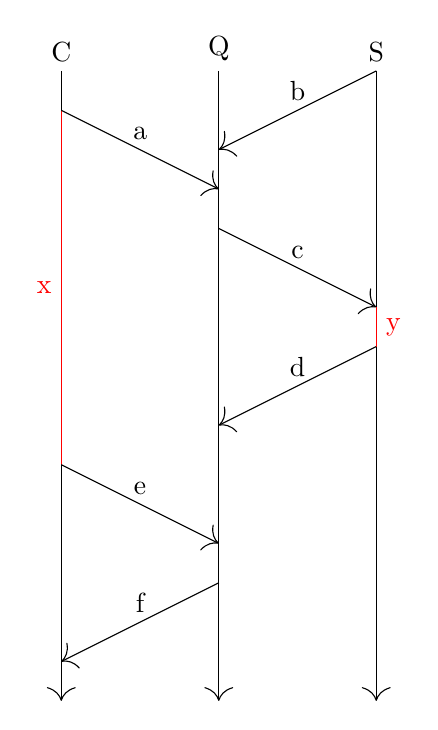
\begin{tikzpicture}
			\draw[-{>[scale=2]}] (0,8) -- (0,0) node[at start, anchor=south] {C};
			\draw[-{>[scale=2]}] (2,8) -- (2,0) node[at start, anchor=south] {Q};
			\draw[-{>[scale=2]}] (4,8) -- (4,0) node[at start, anchor=south] {S};

			\draw[red] (0,7.5) -- (0,3) node[midway, anchor=east] {x};
			\draw[red] (4,5) -- (4,4.5) node[midway, anchor=west] {y};

			\draw[-{>[scale=2]}] (0,7.5) -- (2, 6.5) node[midway, anchor=south] {a};
			\draw[-{>[scale=2]}] (4,8) -- (2, 7) node[midway, anchor=south] {b};
			\draw[-{>[scale=2]}] (2, 6) -- (4, 5) node[midway, anchor=south] {c};
			\draw[-{>[scale=2]}] (4, 4.5) -- (2, 3.5) node[midway, anchor=south] {d};
			\draw[-{>[scale=2]}] (0, 3) -- (2, 2) node[midway, anchor=south] {e};
			\draw[-{>[scale=2]}] (2, 1.5) -- (0, 0.5) node[midway, anchor=south] {f};
		\end{tikzpicture}
	\end{minipage}
	\begin{minipage}{0.6\textwidth}
		\begin{description}
			\item [a] Assignment request message pushed to chunk
				queue
			\item [b] Blocking pop of queue
			\item [c] Message popped from queue
			\item [d] Chunk ID pushed to information reference
				queue
			\item [e] Request for chunk ID creates blocking pop for
				information reference queue
			\item [f] Chunk ID message popped from information
				reference queue
			\item [\textcolor{red}{x}] Creation of chunk object
				containing job ID, but no chunk ID, followed by
				any operations not requiring chunk ID
			\item [\textcolor{red}{y}] Perform operation specified
				by message in \textbf{e}, with assignment
		\end{description}
	\end{minipage}
	\caption{\label{fig:w-o-td}Logical time diagram of chunk assignment for
	server-originated chunk ID}
\end{figure}

\subsection{Chunk Identification}

\subsubsection{Introduction}

The problem of chunk ID origination as discussed in
\href{init-chunk-msg-q-exp.pdf}{Initial Chunk Message Queue Experiments}
dictates much of the client-server communication, as well as the state of
knowledge in the network, given that chunk ID is used as the key to send
messages relevant to a particular chunk.
This document serves to model the differences between naive client-originated
chunk ID's, and server-originated chunk ID's, with an evaluation and proposal
that aims at overcoming the limitations involved in the models.

\subsubsection{Modelling}\label{sec:cid-model}

The models consist of communication over time between a client and a server,
intermediated by a queue server.
The client runs the pseudo-program described in listing \ref{src:client-p},
where variables \texttt{x}, \texttt{y}, and \texttt{z} are chunk references,
and variables \texttt{i} and \texttt{j} are local. 
Every action on distributed chunk references entails pushing a  message to the
queue named by the associated chunk ID, requesting the relevant action to be
performed.

\begin{listing}
\begin{minted}{r}
	y <- f(x)	# dist, no wait
	f(i)		# local
	z <- f(y)	# dist, no wait
	f(j)		# local
	f(z)		# dist, wait
\end{minted}
\caption{Modelled Client Program}\label{src:client-p}
\end{listing}

The server follows a loop of listening on queues relevant to the chunks that it
stores and performing requests from the messages popped in order from them,
through taking the function relayed in the message and performing it on the
local object identified by the chunk ID given by the queue name the message was
popped from.
Without loss of generality, the function \texttt{f} is considered to take
constant time on local objects, and messages likewise have constant latency;
the ratio of latency to operation time is irrelevent to what is demonstrated in
these models.
Assignment, message listening, and message switching by the queue are
considered to be instantaneous events.
The models are depicted as space-time diagrams, with modifications to the
original styling\cite{lamport1978ordering}, including colour coding, where the
colours aim to make each job more distinct.

\subsubsection{Client-Originated Chunk ID}

In the client-originated chunk ID  model, in addition to the generic model
description posed in section \ref{sec:cid-model}, the client sends a chunk ID
as part of its messages if the result of the function on the distributed object
includes assignment.
If there is no assignment, the message includes a job ID instead, naming a job
queue to be monitored by the client.
If the server receives a job ID, it sends the value of the computed function to
the queue with that job ID as it's key, sending no messages otherwise.

A space-time diagram of the client-originated chunk ID model is given in figure
\ref{fig:mci}.

\begin{figure}
	\begin{minipage}{0.6\textwidth}
	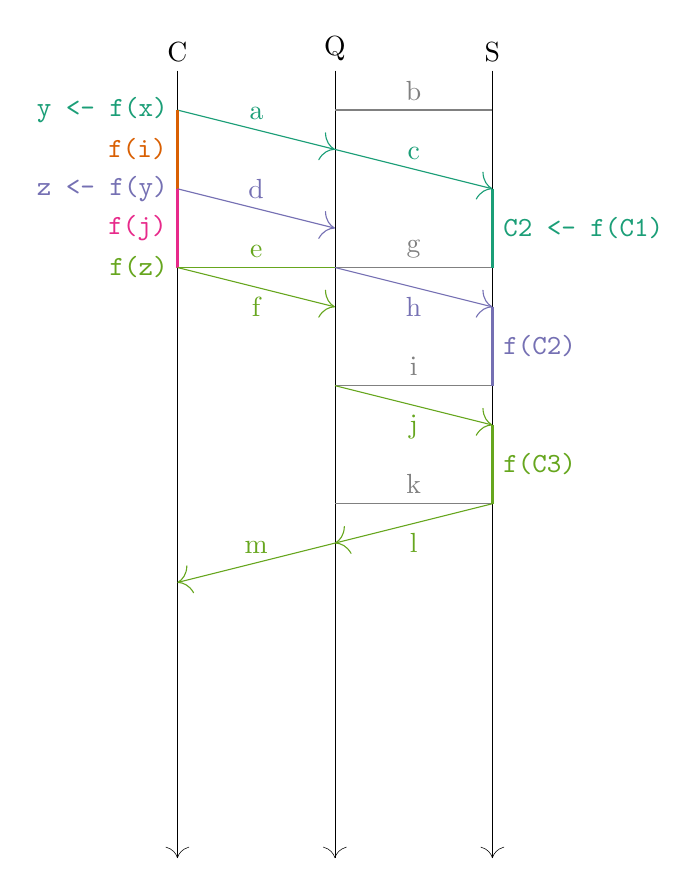
\begin{tikzpicture}
		% nodes
		\draw[very thin,-{>[scale=2]}] (0,10) -- (0,0) 
			node[at start,anchor=south] {C};
		\draw[very thin,-{>[scale=2]}] (2,10) -- (2,0) 
			node[at start,anchor=south] {Q};
		\draw[very thin,-{>[scale=2]}] (4,10) -- (4,0) 
			node[at start,anchor=south] {S};

		% listeners
		\draw[color=mygray] (4,9.5) -- (2,9.5) 
			node[midway,anchor=south] {b};
		\draw[color=dark2-5] (0,7.5) -- (2,7.5) 
			node[midway,anchor=south] {e};
		\draw[color=mygray] (4,7.5) -- (2,7.5) 
			node[midway,anchor=south] {g};
		\draw[color=mygray] (4,6) -- (2,6) 
			node[midway,anchor=south] {i};
		\draw[color=mygray] (4,4.5) -- (2,4.5) 
			node[midway,anchor=south] {k};

		% y <- f(x)
		\draw[-{>[scale=2]},dark2-1] (0,9.5) -- (2,9) 
			node[at start,anchor=east] {\texttt{y <- f(x)}}
			node[midway,anchor=south] {a};
		\draw[-{>[scale=2]},dark2-1] (2,9) -- (4,8.5)
			node[midway,anchor=south] {c};
		\draw[very thick,dark2-1] (4,8.5) -- (4,7.5) 
			node[midway,anchor=west] {\texttt{C2 <- f(C1)}};

		% f(i)
		\draw[very thick,dark2-2] (0,9.5) -- (0,8.5) 
			node[midway,anchor=east] {\texttt{f(i)}};

		% z <- f(y)
		\draw[-{>[scale=2]},dark2-3] (0,8.5) -- (2,8) 
			node[at start,anchor=east] {\texttt{z <- f(y)}}
			node[midway,anchor=south] {d};
		\draw[-{>[scale=2]},dark2-3] (2,7.5) -- (4,7)
			node[midway,anchor=north] {h};
		\draw[very thick,dark2-3] (4,7) -- (4,6) 
			node[midway,anchor=west] {\texttt{f(C2)}};

		% f(j)
		\draw[very thick,dark2-4] (0,8.5) -- (0,7.5)
			node[midway,anchor=east] {\texttt{f(j)}};
			
		% f(z)
		\draw[-{>[scale=2]},dark2-5] (0,7.5) -- (2,7) 
			node[at start,anchor=east] {\texttt{f(z)}}
			node[midway,anchor=north] {f};
		\draw[-{>[scale=2]},dark2-5] (2,6) -- (4,5.5)
			node[midway,anchor=north] {j};
		\draw[very thick,dark2-5] (4,5.5) -- (4,4.5) 
			node[midway,anchor=west] {\texttt{f(C3)}};
		\draw[-{>[scale=2]},dark2-5] (4,4.5) -- (2,4)
			node[midway,anchor=north] {l};
		\draw[-{>[scale=2]},dark2-5] (2,4) -- (0,3.5)
			node[midway,anchor=south] {m};
	\end{tikzpicture}
	\end{minipage}
	\begin{minipage}{0.4\textwidth}
		\begin{description}
			\item [\textcolor{dark2-1}{a}] Push \texttt{<f, chunkID=C2>} to queue \texttt{C1}
			\item [\textcolor{mygray}{b}] Listen to queue \texttt{C1}
			\item [\textcolor{dark2-1}{c}] Pop \texttt{<f, chunkID=C2>} from queue \texttt{C1}
			\item [\textcolor{dark2-3}{d}] Push \texttt{<f, chunkID=C3>} to queue \texttt{C2}
			\item [\textcolor{dark2-5}{e}] Listen to queue \texttt{C3}
			\item [\textcolor{dark2-5}{f}] Push \texttt{<f, jobID=J1>} to queue \texttt{C3}
			\item [\textcolor{mygray}{g}] Listen to queues \texttt{C1, C2}
			\item [\textcolor{dark2-3}{h}] Pop \texttt{<f, chunkID=C3>} from queue \texttt{C2}
			\item [\textcolor{mygray}{i}] Listen to queues \texttt{C1, C2, C3}
			\item [\textcolor{dark2-5}{j}] Pop \texttt{<f, jobID=J1>} from queue \texttt{C3}
			\item [\textcolor{mygray}{k}] Listen to queues \texttt{C1, C2, C3}
			\item [\textcolor{dark2-5}{l}] Push \texttt{<val>} to queue \texttt{J1}
			\item [\textcolor{dark2-5}{m}] Pop \texttt{<val>} from queue \texttt{J1}
		\end{description}
	\end{minipage}
	\caption{\label{fig:mci} Space-Time Diagram of Client-Originated Chunk ID}
\end{figure}

\subsubsection{Server-Originated Chunk ID}

In the server-originated chunk ID model, given that the client doesn't know the
chunk ID of created chunk references, leaving that to the server, it sends out
messages with job IDs, creating chunks references that at first reference the
job ID, but when the actual chunk ID is required, waiting on the job ID queue
for a message containing it's chunk ID.
The server correspondingly sends chunk IDs of each newly assigned chunk to the
job ID queue specified in the request, sending values instead if not directed
to perform assignment.

A diagram of the server-originated chunk ID model is given in figure \ref{fig:msi}.

\setlength{\columnsep}{50pt}
\begin{figure}
	\centering
	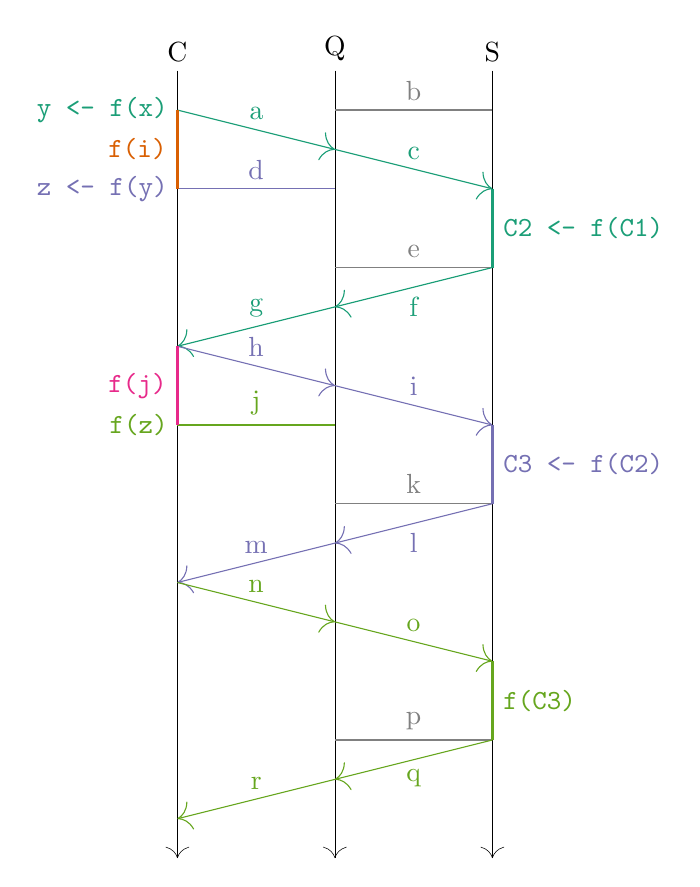
\begin{tikzpicture}
		% nodes
		\draw[very thin,-{>[scale=2]}] (0,10) -- (0,0) 
			node[at start,anchor=south] {C};
		\draw[very thin,-{>[scale=2]}] (2,10) -- (2,0) 
			node[at start,anchor=south] {Q};
		\draw[very thin,-{>[scale=2]}] (4,10) -- (4,0) 
			node[at start,anchor=south] {S};

		% listeners
		\draw[color=mygray] (4,9.5) -- (2,9.5) 
			node[midway,anchor=south] {b};
		\draw[color=dark2-3] (0,8.5) -- (2,8.5) 
			node[midway,anchor=south] {d};
		\draw[color=mygray] (4,7.5) -- (2,7.5) 
			node[midway,anchor=south] {e};
		\draw[color=dark2-5] (0,5.5) -- (2,5.5) 
			node[midway,anchor=south] {j};
		\draw[color=mygray] (4,4.5) -- (2,4.5) 
			node[midway,anchor=south] {k};
		\draw[color=mygray] (4,1.5) -- (2,1.5) 
			node[midway,anchor=south] {p};

		% y <- f(x)
		\draw[-{>[scale=2]},dark2-1] (0,9.5) -- (2,9) 
			node[at start,anchor=east] {\texttt{y <- f(x)}}
			node[midway,anchor=south] {a};
		\draw[-{>[scale=2]},dark2-1] (2,9) -- (4,8.5)
			node[midway,anchor=south] {c};
		\draw[very thick,dark2-1] (4,8.5) -- (4,7.5) 
			node[midway,anchor=west] {\texttt{C2 <- f(C1)}};
		\draw[-{>[scale=2]},dark2-1] (4,7.5) -- (2,7) 
			node[midway,anchor=north] {f};
		\draw[-{>[scale=2]},dark2-1] (2,7) -- (0,6.5)
			node[midway,anchor=south] {g};

		% f(i)
		\draw[very thick,dark2-2] (0,9.5) -- (0,8.5)
			node[midway,anchor=east] {\texttt{f(i)}};

		% z <- f(y)
		\node[anchor=east,color=dark2-3] at (0,8.5) {\texttt{z <- f(y)}};
		\draw[-{>[scale=2]},dark2-3] (0,6.5) -- (2,6) 
			node[midway,anchor=south] {h};
		\draw[-{>[scale=2]},dark2-3] (2,6) -- (4,5.5)
			node[midway,anchor=south] {i};
		\draw[very thick,dark2-3] (4,5.5) -- (4,4.5) 
			node[midway,anchor=west] {\texttt{C3 <- f(C2)}};
		\draw[-{>[scale=2]},dark2-3] (4,4.5) -- (2,4) 
			node[midway,anchor=north] {l};
		\draw[-{>[scale=2]},dark2-3] (2,4) -- (0,3.5)
			node[midway,anchor=south] {m};

		% f(j)
		\draw[very thick,dark2-4] (0,6.5) -- (0,5.5)
			node[midway,anchor=east] {\texttt{f(j)}};
			
		% f(z)
		\node[anchor=east,color=dark2-5] at (0,5.5) {\texttt{f(z)}};
		\draw[-{>[scale=2]},dark2-5] (0,3.5) -- (2,3) 
			node[midway,anchor=south] {n};
		\draw[-{>[scale=2]},dark2-5] (2,3) -- (4,2.5)
			node[midway,anchor=south] {o};
		\draw[very thick,dark2-5] (4,2.5) -- (4,1.5) 
			node[midway,anchor=west] {\texttt{f(C3)}};
		\draw[-{>[scale=2]},dark2-5] (4,1.5) -- (2,1) 
			node[midway,anchor=north] {q};
		\draw[-{>[scale=2]},dark2-5] (2,1) -- (0,0.5)
			node[midway,anchor=south] {r};
	\end{tikzpicture}
	\begin{multicols}{2}
		\begin{description}
			\item [\textcolor{dark2-1}{a}] Push \texttt{<f, jobID=J1>} to queue \texttt{C1}
			\item [\textcolor{mygray}{b}] Listen to queue \texttt{C1}
			\item [\textcolor{dark2-1}{c}] Pop \texttt{<f, jobID=J1>} from queue \texttt{C1}
			\item [\textcolor{dark2-3}{d}] Listen to queue \texttt{J1}
			\item [\textcolor{mygray}{e}] Listen to queues \texttt{C1, C2}
			\item [\textcolor{dark2-1}{f}] Push \texttt{<chunkID=C2>} to queue \texttt{J1}
			\item [\textcolor{dark2-1}{g}] Pop \texttt{<chunkID=C2>} from queue \texttt{J1}
			\item [\textcolor{dark2-3}{h}] Push \texttt{<f, jobID=J2>} to queue \texttt{C2}
			\item [\textcolor{dark2-3}{i}] Pop \texttt{<f, jobID=J2>} from queue \texttt{C2}
			\item [\textcolor{dark2-5}{j}] Listen to queue \texttt{J2}
			\item [\textcolor{mygray}{k}] Listen to queues \texttt{C1, C2, C3}
			\item [\textcolor{dark2-3}{l}] Push \texttt{<chunkID=C3>} to queue \texttt{J2}
			\item [\textcolor{dark2-3}{m}] Pop \texttt{<chunkID=C3>} from queue \texttt{J2}
			\item [\textcolor{dark2-5}{n}] Push \texttt{<f, jobID=J3>} to queue \texttt{C3}
			\item [\textcolor{dark2-5}{o}] Pop \texttt{<f, jobID=J3>} from queue \texttt{C3}
			\item [\textcolor{mygray}{p}] Listen to queues \texttt{C1, C2, C3}
			\item [\textcolor{dark2-5}{q}] Push \texttt{<val>} to queue \texttt{J3}
			\item [\textcolor{dark2-5}{r}] Pop \texttt{<val>} from queue \texttt{J3}
		\end{description}
	\end{multicols}
	\caption{\label{fig:msi} Space-Time Diagram of Server-Originated Chunk ID}
\end{figure}

An important aspect of figure \ref{fig:msi} is the fact that the client has to
wait to get the chunk ID's of the chunk references \texttt{y} and \texttt{z}
before it can push requests to their relevent queues, hence the delay between
the communications labelled in the diagram as \textcolor{dark2-3}{\textbf{d}}
and \textcolor{dark2-3}{\textbf{h}}; the client still needs to receive
\textcolor{dark2-1}{\textbf{g}}, which contains the necessary chunk ID.

\subsubsection{Evaluation}\label{sec:mod-eval}

Clearly, the server-originated chunks result in significantly more waiting on
the client end, as the chunk ID needs to be attained for every operation on the
associated chunk, which is only able to be acquired after completing the
function.

The server could in theory send the chunk ID prior to performing the requested
operation, but that leads to significant issues when the operation results in
error, as it is difficult to communicate such a result back to the client after
performing the function.
Despite the reduced time spent blocking, the client-originated chunk ID
modelled also has issue with errors; consider if the \texttt{x <- f(y)} had
been faulty, with the resultant operation of \texttt{f(C1)} rendering an error.
This would not be determined by the client untile the completion of
\texttt{f(z)}, in which an error would presumably result.
Worse, if the chunk reference \texttt{x} was given as an additional argument to
another server, which in turn requested the chunk \texttt{C1} from the node
\texttt{C1} resided upon, the error would propagate, with the source of the
error being exceedingly difficult to trace.

\subsubsection{Proposal}

A potential solution to the problems of the models posed in section
\ref{sec:mod-eval} is to treat chunk reference objects somewhat like futures,
which have a state of \texttt{resolved} or \texttt{unresolved}, with failures
also encapsulated in the object upon resolution\cite{bengtsson19:_futur_r}.

If chunk ID is client-originated, then its outgoing messages can also supply a
job ID for the server to push a message to upon completion that the client can
in turn refer to, in order to check resolution status as well as any potential
errors.

This would capture the benefits of the modelled client-originated chunk ID in
reduces wait time, with the robustness of server-originated ID in signalling of
errors.
The introduction of future terminology of \texttt{resolved()}, as well as
additional slots in a chunk to determine resolution state, as well as the use
of job ID queues for more than just value returns will be sufficient to
implement such a design.
The asynchrony may lead to non-deterministic outcomes in the case of failure,
but the use of \texttt{resolved()} and it's associated barrier procedure,
\texttt{resolve()} will enable the forcing of a greater degree of synchrony,
and allow tracing of errors back to their source in a more reliable manner.

A diagram of the proposed model, along with an additional \texttt{resolved(x)}
step, is given in \ref{fig:masi}

\begin{figure}
	\centering
	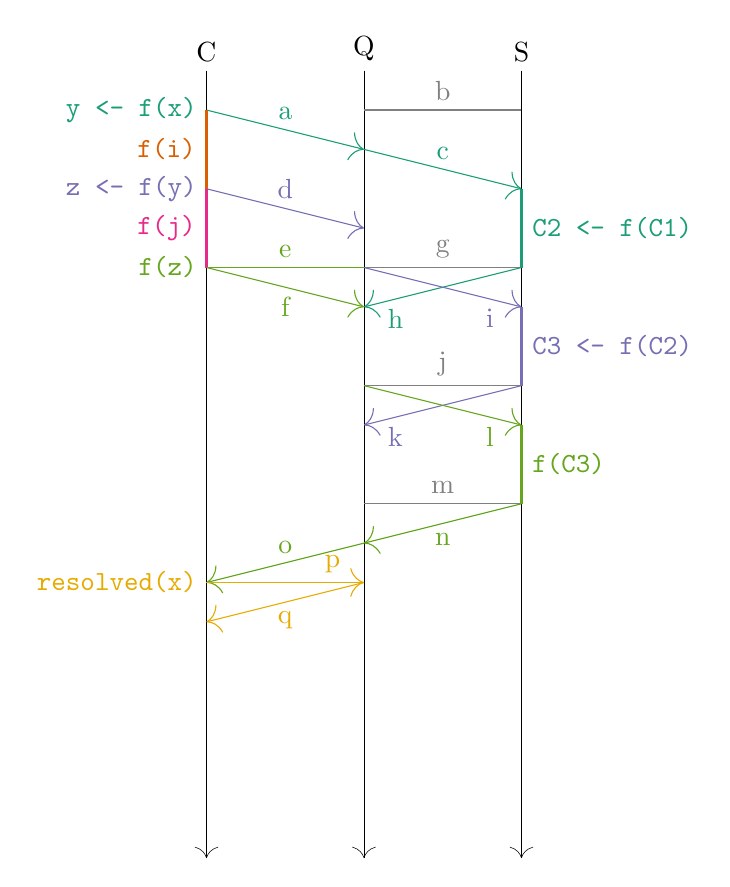
\begin{tikzpicture}
		% nodes
		\draw[very thin,-{>[scale=2]}] (0,10) -- (0,0) 
			node[at start,anchor=south] {C};
		\draw[very thin,-{>[scale=2]}] (2,10) -- (2,0) 
			node[at start,anchor=south] {Q};
		\draw[very thin,-{>[scale=2]}] (4,10) -- (4,0) 
			node[at start,anchor=south] {S};

		% listeners
		\draw[color=mygray] (4,9.5) -- (2,9.5) 
			node[midway,anchor=south] {b};
		\draw[color=dark2-5] (0,7.5) -- (2,7.5) 
			node[midway,anchor=south] {e};
		\draw[color=mygray] (4,7.5) -- (2,7.5) 
			node[midway,anchor=south] {g};
		\draw[color=mygray] (4,6) -- (2,6) 
			node[midway,anchor=south] {j};
		\draw[color=mygray] (4,4.5) -- (2,4.5) 
			node[midway,anchor=south] {m};

		% y <- f(x)
		\draw[-{>[scale=2]},dark2-1] (0,9.5) -- (2,9) 
			node[at start,anchor=east] {\texttt{y <- f(x)}}
			node[midway,anchor=south] {a};
		\draw[-{>[scale=2]},dark2-1] (2,9) -- (4,8.5)
			node[midway,anchor=south] {c};
		\draw[very thick,dark2-1] (4,8.5) -- (4,7.5) 
			node[midway,anchor=west] {\texttt{C2 <- f(C1)}};
		\draw[-{>[scale=2]},dark2-1] (4,7.5) -- (2,7)
			node[pos=0.8,anchor=north] {h};

		% f(i)
		\draw[very thick,dark2-2] (0,9.5) -- (0,8.5) 
			node[midway,anchor=east] {\texttt{f(i)}};

		% z <- f(y)
		\draw[-{>[scale=2]},dark2-3] (0,8.5) -- (2,8) 
			node[at start,anchor=east] {\texttt{z <- f(y)}}
			node[midway,anchor=south] {d};
		\draw[-{>[scale=2]},dark2-3] (2,7.5) -- (4,7)
			node[pos=0.8,anchor=north] {i};
		\draw[very thick,dark2-3] (4,7) -- (4,6) 
			node[midway,anchor=west] {\texttt{C3 <- f(C2)}};
		\draw[-{>[scale=2]},dark2-3] (4,6) -- (2,5.5)
			node[pos=0.8,anchor=north] {k};

		% f(j)
		\draw[very thick,dark2-4] (0,8.5) -- (0,7.5)
			node[midway,anchor=east] {\texttt{f(j)}};
			
		% f(z)
		\draw[-{>[scale=2]},dark2-5] (0,7.5) -- (2,7) 
			node[at start,anchor=east] {\texttt{f(z)}}
			node[midway,anchor=north] {f};
		\draw[-{>[scale=2]},dark2-5] (2,6) -- (4,5.5)
			node[pos=0.8,anchor=north] {l};
		\draw[very thick,dark2-5] (4,5.5) -- (4,4.5) 
			node[midway,anchor=west] {\texttt{f(C3)}};
		\draw[-{>[scale=2]},dark2-5] (4,4.5) -- (2,4)
			node[midway,anchor=north] {n};
		\draw[-{>[scale=2]},dark2-5] (2,4) -- (0,3.5)
			node[midway,anchor=south] {o};

		% resolved(x)
		\draw[-{>[scale=2]},dark2-6] (0,3.5) -- (2,3.5) 
			node[at start,anchor=east] {\texttt{resolved(x)}}
			node[pos=0.8,anchor=south] {p};
		\draw[-{>[scale=2]},dark2-6] (2,3.5) -- (0,3)
			node[midway,anchor=north] {q};
	\end{tikzpicture}
	\setlength{\columnsep}{50pt}
	\begin{multicols}{2}
		\begin{description}
			\item [\textcolor{dark2-1}{a}] Push \texttt{<f, chunkID=C2, jobID=J1>} to queue \texttt{C1}
			\item [\textcolor{mygray}{b}] Listen to queue \texttt{C1}
			\item [\textcolor{dark2-1}{c}] Pop \texttt{<f, chunkID=C2, jobID=J1>} from queue \texttt{C1}
			\item [\textcolor{dark2-3}{d}] Push \texttt{<f, chunkID=C3 jobID=J2>} to queue \texttt{C2}
			\item [\textcolor{dark2-5}{e}] Listen to queue \texttt{J3}
			\item [\textcolor{dark2-5}{f}] Push \texttt{<f, jobID=J3>} to queue \texttt{C3}
			\item [\textcolor{mygray}{g}] Listen to queues \texttt{C1, C2}
			\item [\textcolor{dark2-1}{h}] Push \texttt{<success>} to queue \texttt{J1}
			\item [\textcolor{dark2-3}{i}] Pop \texttt{<f, chunkID=C3, jobID=J2>} from queue \texttt{C2}
			\item [\textcolor{mygray}{j}] Listen to queues \texttt{C1, C2, C3}
			\item [\textcolor{dark2-3}{k}] Push \texttt{<success>} to queue \texttt{J2}
			\item [\textcolor{dark2-5}{l}] Pop \texttt{<f, jobID=J3>} from queue \texttt{C3}
			\item [\textcolor{mygray}{m}] Listen to queues \texttt{C1, C2, C3}
			\item [\textcolor{dark2-5}{n}] Push \texttt{<val>} to queue \texttt{J3}
			\item [\textcolor{dark2-5}{o}] Pop \texttt{<val>} from queue \texttt{J3}
			\item [\textcolor{dark2-6}{p}] Listen to queue \texttt{J1}
			\item [\textcolor{dark2-6}{q}] Pop \texttt{<success>} from queue \texttt{J1}
		\end{description}
	\end{multicols}
	\caption{\label{fig:masi} Space-Time Diagram of Proposed Amended Server-Originated Chunk ID}
\end{figure}

Note in the diagram how the message sent by the server as part of
\textcolor{dark2-1}{h} is listened for in \textcolor{dark2-6}{p} and popped to
determine status of resolution in \textcolor{dark2-6}{q}.
Such job ID queues will mostly remain un-popped, so it may be worth associating
an expiry time with them.

\subsection{Message Queue System Architecture}

\subsubsection{Introduction}

The purpose of this report is to outline the workings of the present
architecture at the chunk layer.
This follows the experiments recorded in
\href{init-chunk-msg-q-exp.pdf}{``Initial chunk message queue experiments''},
with the final experiment providing the basis for modifications allowing a
self-sufficient distObj package, along with the modifications recommended by
\href{chunk-id-orig.pdf}{``Chunk ID Origination''}.

The functionality of the package can be demonstrated through installing distObj
and it's prerequisites, and, with a running \texttt{redis-server}, evaluating
\mintinline{r}{demo("chunk-server", package="distObj")} in one R
process, and \mintinline{r}{demo("chunk-client", package="distObj")} in
another process on the same host, stepping through the ``chunk-client'' demo to
control operation, with the results appearing similar to those recorded in
table \ref{tab:chunk-comm}.

The full source code of the implementation is given in section
\ref{sec:listings} as listings \ref{src:chunk-client}-\ref{src:chunk-util}.

\subsubsection{Overview}

The central units of this distributed system are a client, a queue server, and
a chunk server, as demonstrated in figure \ref{fig:chunk-arch}.

The client contains chunk references, which can be passed as arguments to
\texttt{do.call.chunkRef}, alongside some function, in order to begin the
process of evaluation, and if assignment is desired, producing a new chunk
reference to continue computation with on the client end while the evaluation
continues on the other units.

\texttt{do.call.chunkRef} composes a message based on the request, pushing that
to the queue identified by the chunk ID contained in the chunk reference, with
the queue existing on some central queue server.

The chunk server concurrently monitors all queues identified by the chunk ID's
of the chunks that the chunk server stores in a local chunk table.
It pops the message off the related queue, and has \texttt{do.call.chunk}
evaluate the function on the chunk, with various options determined by the
content of the received message.

The chunk server pushes some response message to the queue associated with that
particular job through a unique job ID, which may be picked up later by the
client later.

\begin{figure}
	\centering
	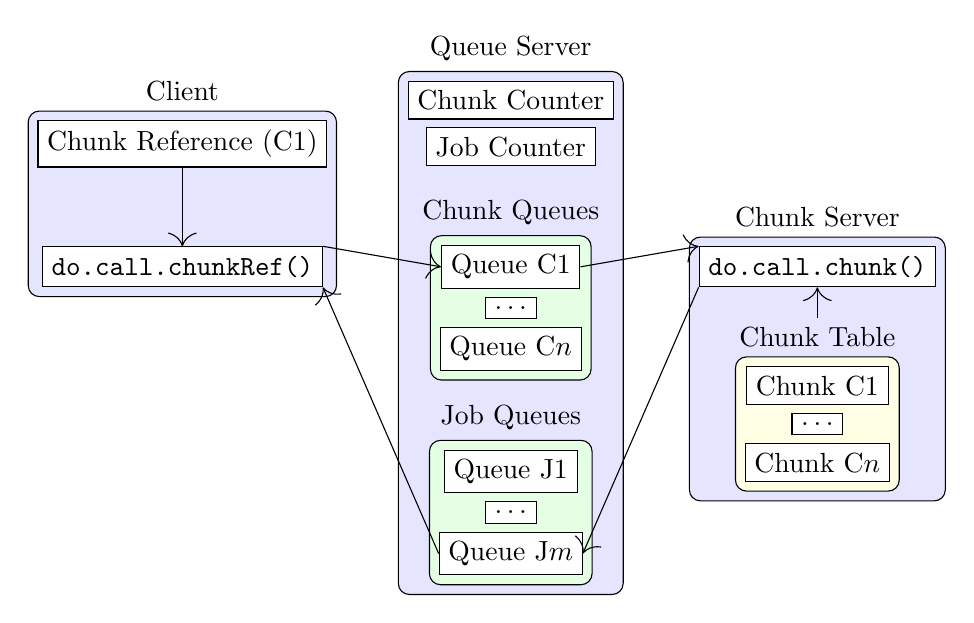
\begin{tikzpicture}[scale=0.5]
		% client
		\node[object] (chunkref) {Chunk Reference (C1)};
		\node[proc,below=of chunkref] (docallcr) {\texttt{do.call.chunkRef()}};

		% Queue server
		%% chunk queues
		\node[queue,right=\commdist of docallcr] (c1) {Queue C1};
		\node[queue,below=\blockdist of c1] (cdotdot) {\(\dots\)};
		\node[queue,below=\blockdist of cdotdot] (cn) {Queue C\(n\)};
		%% job queues
		\node[queue,below=of cn] (j1) {Queue J1};
		\node[queue,below=\blockdist of j1] (jdotdot) {\(\dots\)};
		\node[queue,below=\blockdist of jdotdot] (jm) {Queue J\(m\)};
		%% counters
		\node[counter,above=of c1] (jc) {Job Counter};
		\node[counter,above=\blockdist of jc] (cc) {Chunk Counter};

		% Chunk server
		\node[proc,right=\commdist of c1] (docallc) {\texttt{do.call.chunk()}};
		\node[object,below=of docallc] (chunk1) {Chunk C1};
		\node[object,below=\blockdist of chunk1] (chunkdotdot) {\(\dots\)};
		\node[object,below=\blockdist of chunkdotdot] (chunkn) {Chunk C\(n\)};

		\begin{pgfonlayer}{categories}
			\node[category,fit=(c1)(cdotdot)(cn),label={[name=cq] Chunk Queues}] (chunkq) {};
			\node[category,fit=(j1)(jdotdot)(jm),label={[name=jq] Job Queues}] (jobq) {};
			\node[table,fit=(chunk1)(chunkn),label={[name=ct] Chunk Table}] (chunkt) {};
		\end{pgfonlayer}

		\begin{pgfonlayer}{units}
			\node[unit,fit=(chunkref)(docallcr),label={Client}] (client) {};
			\node[unit,fit=(cc)(chunkq)(jobq),label={Queue Server}] (qserv) {};
			\node[unit,fit=(docallc)(chunkt),label={Chunk Server}] (cserv) {};
		\end{pgfonlayer}
		
		% Connections
		\draw[mypath] (chunkref) -- (docallcr);
		\draw[mypath] (docallcr.north east) -- (c1.west);
		\draw[mypath] (jm.west) -- (docallcr.south east);
		\draw[mypath] (c1.east) -- (docallc.north west);
		\draw[mypath] (docallc.south west) -- (jm.east);
		\draw[mypath] (ct.north) -- (docallc.south);
	\end{tikzpicture}
	\caption{\label{fig:chunk-arch} An outline of the architecture of the
	chunk component in the distributed system}
\end{figure}

\newpage
\subsubsection{Object Formats}
The fields belonging to a \texttt{chunkRef} object are the following:
\begin{description}
	\item[\texttt{CHUNK\_ID}] The name of the queue to post messages to, as
		well as the name of the chunk existing on the server to perform
		operations upon.
	\item[\texttt{JOB\_ID}] The name of the queue to pop a response from.
	\item[\texttt{RESOLUTION}] The status of whether a response has been
		heard from the server, taking the values ``UNRESOLVED'',
		``RESOLVED'', or a condition object signalling an error.
	\item[\texttt{PREVIEW}] A small preview of the complete object for use
		in printing.
\end{description}

Messages all belong to the \texttt{msg} class, and are currently categorised as
either requests, or responses, with the following fields:\\

Request:
\begin{description}
	\item[\texttt{OP}] Directive for server to carry out, e.g. ``ASSIGN''.
	\item[\texttt{FUN}] Function object or character naming function to
		perform on the chunk.
	\item[\texttt{CHUNK}] Chunk Reference for the server to attain
		information from.
	\item[\texttt{JOB\_ID}] The name of the queue to push a response to.
	\item[\texttt{DIST\_ARGS}] Additional distributed arguments to the
		function.
	\item[\texttt{STATIC\_ARGS}] Additional static arguments to the
		function.
\end{description}

Response:
\begin{description}
	\item[\texttt{RESOLUTION}] Resolution status; either ``RESOLVED'', or a
		condition object detailing failure due to error.
	\item[\texttt{PREVIEW}]  A small snapshot of the completed object for
		use in printing chunk references.
\end{description}

\subsubsection{Demonstration of Communication}

The table \ref{tab:chunk-comm} shows a demonstration of verbose communication
between a client and a server, corresponding to the listings
\ref{src:chunk-client} and \ref{src:chunk-server} respectively.
In this demo, the server was started immediately prior to the client, being
backgrounded, and initial setup was performed in both as per the listings
referred to prior.

\begin{table}
	\def\clientcolour{mybrown}
	\def\servercolour{mynavy}
	\centering
	\begin{tabularx}{\textwidth}{lX}
		\toprule
		Time (secs)  & Message/\texttt{expression} (\textcolor{\clientcolour}{client}/\textcolor{\servercolour}{server}) \\
		\midrule
		0        & \textcolor{\servercolour}{Assigned chunk to ID: chunk1 in chunk table} \\
			 & \textcolor{\clientcolour}{\texttt{x <- do.call.chunkRef(what="expm1", chunkArg=chunk1)} } \\
		0.001664 & \textcolor{\clientcolour}{Attained job ID:  J1} \\
		0.002719 & \textcolor{\clientcolour}{Attained Chunk ID:  C1} \\
		0.00292  & \textcolor{\clientcolour}{Requesting to perform function expm1 on chunk chunk1 with assignment} \\
		0.003521 & \textcolor{\clientcolour}{writing message: ASSIGN expm1 <environment: 0x55cc164cb8c8> NULL NULL J1 C1 to queue belonging to chunk" chunk1 "} \\
		0.0051   & \textcolor{\clientcolour}{Producing new chunk reference with chunk ID: C1 and job ID: J1} \\
			 & \textcolor{\clientcolour}{\texttt{y <- do.call.chunkRef("as.Date", x)}} \\
		0.005679 & \textcolor{\clientcolour}{Attained job ID:  J2} \\
		0.005986 & \textcolor{\clientcolour}{Attained Chunk ID:  C2} \\
		0.006159 & \textcolor{\clientcolour}{Requesting to perform function as.Date on chunk C1 with assignment} \\
		0.006622 & \textcolor{\clientcolour}{writing message: ASSIGN as.Date <environment: 0x55cc165d0808> NULL NULL J2 C2 to queue belonging to chunk" C1 "} \\
		0.007351 & \textcolor{\clientcolour}{Producing new chunk reference with chunk ID: C2 and job ID: J2} \\
			 & \textcolor{\clientcolour}{\texttt{expm1(1:10)}} \\
			 & \textcolor{\clientcolour}{\texttt{x}} \\
		0.007811 & \textcolor{\clientcolour}{Chunk not yet resolved. Resolving...} \\
		0.008025 & \textcolor{\clientcolour}{Awaiting message on queues: J1} \\
		0.028962 & \textcolor{\servercolour}{Awaiting message on queues: chunk1} \\
		0.029668 & \textcolor{\servercolour}{Received message: ASSIGN expm1 <environment: 0x55a7a47917e0> NULL NULL J1 C1} \\
		0.030912 & \textcolor{\servercolour}{Requested to perform function expm1} \\
		0.031777 & \textcolor{\servercolour}{writing message: RESOLVED 1.718282, 6.389056, ..., to queue belonging to chunk" J1 "} \\
		0.03237  & \textcolor{\servercolour}{Assigned chunk to ID: C1 in chunk table} \\
		0.032679 & \textcolor{\servercolour}{Awaiting message on queues: C1     chunk1} \\
		0.032695 & \textcolor{\clientcolour}{Received message: RESOLVED 1.718282, 6.389056, ... } \\
		0.033206 & \textcolor{\servercolour}{Received message: ASSIGN as.Date <environment: 0x55a7a4863308> NULL NULL J2 C2} \\
			 & \textcolor{\clientcolour}{\texttt{do.call.chunkRef("identity", x, assign=FALSE)}} \\
		0.033662 & \textcolor{\clientcolour}{Attained job ID:  J3} \\
		0.033825 & \textcolor{\servercolour}{Requested to perform function as.Date} \\
		0.033893 & \textcolor{\clientcolour}{Requesting to perform function identity on chunk C1 with no assignment} \\
		0.034363 & \textcolor{\clientcolour}{writing message: DOFUN identity <environment: 0x55cc165d0808> NULL NULL J3 NULL to queue belonging to chunk" C1 "} \\
		0.034363 & \textcolor{\servercolour}{Error occured: 'origin' must be supplied} \\
		0.034655 & \textcolor{\servercolour}{writing message: 'origin' must be supplied, as.Date.numeric(c(...)) to queue belonging to chunk" J2 "} \\
		0.03519  & \textcolor{\clientcolour}{Awaiting message on queues: J3} \\
		0.035544 & \textcolor{\servercolour}{Assigned chunk to ID: C2 in chunk table} \\
		0.035747 & \textcolor{\servercolour}{Awaiting message on queues: C1     C2     chunk1} \\
		0.036224 & \textcolor{\servercolour}{Received message: DOFUN identity <environment: 0x55a7a48ed380> NULL NULL J3 NULL} \\
		0.036737 & \textcolor{\servercolour}{Requested to perform function identity} \\
		0.037004 & \textcolor{\servercolour}{writing message: 1.718282, 6.389056, ..., to queue belonging to chunk" J3 "} \\
		0.03742  & \textcolor{\servercolour}{Awaiting message on queues: C1     C2     chunk1} \\
		0.037675 & \textcolor{\clientcolour}{Received message: 1.718282, 6.389056, ... } \\
			 & \textcolor{\clientcolour}{\texttt{resolve(y)}} \\
		0.038197 & \textcolor{\clientcolour}{Chunk not yet resolved. Resolving...} \\
		0.038325 & \textcolor{\clientcolour}{Awaiting message on queues: J2} \\
		0.038825 & \textcolor{\clientcolour}{Received message: 'origin' must be supplied, as.Date.numeric(c(...))} \\
		\bottomrule
	\end{tabularx}
	\caption{Communication between a client and server}
	\label{tab:chunk-comm}
\end{table}

\subsubsection{Next Steps}

The next step is to experiment with aggregates of chunks, as distributed objects.
A significant component of this involves point-to-point chunk movement, between multiple servers.
The package ``osrv'' looks to satisfy much of the infrastructure required for
this, with particular experiments to be dedicated specifically to establishing
a fast and reliable mechanism for co-ordination and data movement in the system.

\subsection{Distributed Objects in the Message Queue System}

\subsubsection{Introduction}

Building on the infrastructure outlined in \href{chunk-report.pdf}{Report on
Current Chunk Architecture}, the aggragation of chunks as a distributed object
is a logical continuation, and this document serves to record experimentation
in the creation of such a feature.

For our purposes, a distributed object and it's reference is defined
conceptually as the following:

\begin{definition}
	\label{distobj}
	A distributed object is a set \(D\) of chunks \(c_1, c_2, \dots, c_n\),
	with some total ordering defined on the chunks. 
	In a corresponding manner, distributed object \textit{references} are
	sets of chunk references, along with an ordering on the chunk
	references to match that of the chunks composing the referent
	distributed object.
\end{definition}

This definition will be expanded upon and serve to inform the nature of the
following experiments.

\subsubsection{Formation}

The first experiment is the most important, in composing a basic distributed
object reference along with sufficient infrastructure to allow for operations
to take place on the referent chunks composing the conceptual distributed
object.
This section sees an informal description of the initial model, as well as
issues in such a model, along with proposed solutions and an example
implementation.

\subsubsection{Model Description}

Following definition \ref{distobj}, as well as the existing infrastructure
provided and outlined in \href{chunk-report.pdf}{Chunk Report}, the distributed
object reference consists of an environment containing a list of chunk
references.
The capacity for further components is reserved, however the prime information
is encapsulated within the chunk references.

Some changes are made to the chunk references as described in
\href{chunk-report.pdf}{Chunk Report}, based on the need for decoupling data
from process when communicating among client and server.
This takes the principal form of removing the job ID in favour of posting chunk
information directly to the distributed table as keys.
In this manner, all necessary information relating to a chunk ID is
encapsulated in the chunk reference, with no need to couple this with job ID's
and the implied necessity of a job reference.
As an example, the resolution status of a chunk ID (whether it has actually
been created) is posted as a resolution key identified by the chunk ID in the
distributed table, rather than being rolled into a message object and sent to a
job ID queue.
This change has further motivations in allowing access to attributes of a chunk
that may resolve asynchronously, by nodes other than the original requesting
client.
For example, an as-yet undefined alignment process requires knowledge of chunk
sizes, and may be taking place on a node separate and prior to determination of
such information on another node, which upon realisation, posts the chunk size
data to the distributed table, and the node performing alignment may now have
access to that information despite not being the original requesting client.
This would not be possible were the job queue concept still used, as the chunk
reference on the aligning node wouldn't have the ability to access the job
queue, for lack of knowledge as well as the destruction it would cause by
obstructing the original client in it's intended pop of the jobID queue.

In addition to the changes to the chunk reference, there is now the essential
need for further information in the way chunks relate to each other as parts of
a greater whole.
This is a heavily language-dependent aspect, as it relies on R's paradigmatic
nature of being array-oriented.
R takes it's array-oriented style from S, which was in turn influenced by
Iverson's APL and Backus' FORTRAN, both heavily
array-oriented\cite{becker1994shistory}\cite{iverson2007notation}.
A central feature of array-oriented languages involves ``parallel'' (in array,
not computational terms) operation on arrays with elements in corresponding
indices; beyond serving as a store of information, arrays can be comparable
with each other, and operations performed on associated elements between them.
This is obvious even in simple expressions such as 
\mintinline{r}{1:10 + 11:20}, wherein vectors are operated upon in
adjacently.
This expectation raises a problem for operations on multiple distributed
objects, where if the chunks holding adjacent elements are required for a
multivariate operation yet exist on entirely separate nodes, there is no
possibility for executing the operation absent movement of data.

The movement of data is to a degree not the most difficult aspect, but an
immediate issue is the efficient co-ordination of such data movement, a process
described here as \textit{alignment}.
Alignment requires all elements adjacent and relevant to other elements in an
operation to be located on the same node for processing.
Such a task is further compounded by the standard operation of recycling,
wherein arrays of shorter length than others are copied end-to-end in order to
achieve the same size.
An example is given in the expression \mintinline{r}{1:10 + 1:2}, where
the second vector of length 2 is repeated 4 additional times in order to match
the size of the larger.
This is a sufficiently common task that the system should provide it by default
when moving data.

With these problems stated, a fuller description of the base model can now be
entered into, with figure \ref{fig:distobj} accompanying.

\begin{figure}
	\centering
	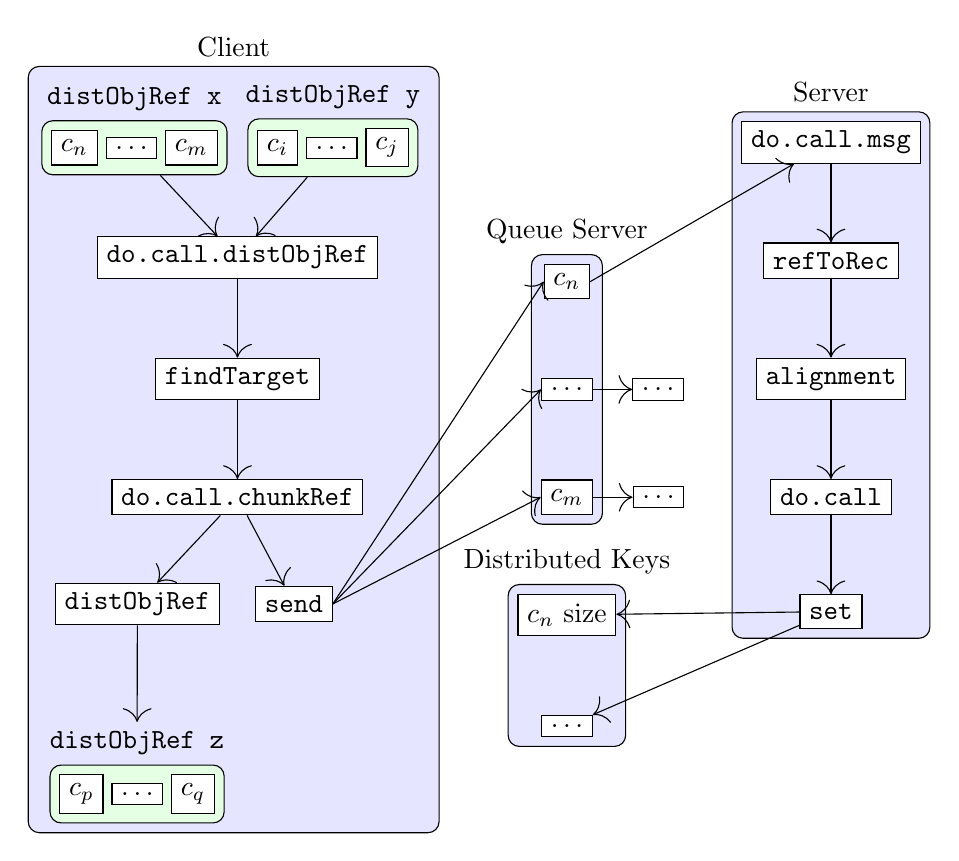
\begin{tikzpicture}
		% distobjrefs
		\node[object] (cn) {\(c_n\)};
		\node[object,right=\blockdist of cn] (cndot) {\(\dots\)};
		\node[object,right=\blockdist of cndot] (cm) {\(c_m\)};
		\node[object,right={5*\blockdist} of cm] (ci) {\(c_i\)};
		\node[object,right=\blockdist of ci] (cidot) {\(\dots\)};
		\node[object,right=\blockdist of cidot] (cj) {\(c_j\)};
		\path (cm.east) -- (ci.west) node(midclient) [midway] {};

		% client args
		\node[proc,below=of midclient] (dcdor) {\texttt{do.call.distObjRef}};
		\node[proc,below=of dcdor] (ft) {\texttt{findTarget}};
		\node[proc,below=of ft] (dccr) {\texttt{do.call.chunkRef}};
		\node[below=of dccr] (midlowcl) {};
		\node[proc,left=\blockdist of midlowcl] (dor) {\texttt{distObjRef}};
		\node[proc,right=\blockdist of midlowcl] (sendreq) {\texttt{send}};

		\node[object,below=2 of dor] (cpdot) {\(\dots\)};
		\node[object,left=\blockdist of cpdot] (cp) {\(c_p\)};
		\node[object,right=\blockdist of cpdot] (cq) {\(c_q\)};

		% chunk queues
		\node[queue,right={1.5*\commdist} of dccr] (cmq) {\(c_m\)};
		\node[queue,above=of cmq] (cmdotq) {\(\dots\)};
		\node[queue,above=of cmdotq] (cnq) {\(c_n\)};
		\node[queue,right={5*\blockdist} of cmdotq] (cmdotqdot) {\(\dots\)};
		\node[queue,right={5*\blockdist} of cmq] (cmqdot) {\(\dots\)};

		% server args
		\node[proc,right={1.5*\commdist} of cmq] (dc) {\texttt{do.call}};
		\node[proc,above=of dc] (alignment) {\texttt{alignment}};
		\node[proc,above=of alignment] (r2r) {\texttt{refToRec}};
		\node[proc,above=of r2r] (dcm) {\texttt{do.call.msg}};
		\node[proc,below=of dc] (set) {\texttt{set}};

		% metadata
		\node[object,below=of cmq] (cns) {\(c_n\) size};
		\node[object,below=of cns] (cdots) {\(\dots\)};

		\begin{pgfonlayer}{categories}
			\node[category,fit=(cn)(cndot)(cm),label={[name=dnl] \texttt{distObjRef x}}] (dn) {};
			\node[category,fit=(ci)(cidot)(cj),label={[name=dil] \texttt{distObjRef y}}] (di) {};
			\node[category,fit=(cp)(cpdot)(cq),label={[name=dql]\texttt{distObjRef z}}] (dq) {};
		\end{pgfonlayer}

		\begin{pgfonlayer}{units}
			\node[unit,fit=(dnl)(dil)(dor)(sendreq)(dq)(dql),label={[name=cl] Client}] (c) {};
			\node[unit,fit=(cmq)(cnq),label={[name=qsl] Queue Server}] (qs) {};
			\node[unit,fit=(cns)(cdots),label={[name=setsl] Distributed Keys}] (sets) {};
			\node[unit,fit=(dcm)(set),label={[name=sl] Server}] (s) {};
		\end{pgfonlayer}

		\draw[mypath] (dn) -- (dcdor);
		\draw[mypath] (di) -- (dcdor);
		\draw[mypath] (dcdor) -- (ft);
		\draw[mypath] (ft) -- (dccr);
		\draw[mypath] (dccr) -- (dor);
		\draw[mypath] (dccr) -- (sendreq);
		\draw[mypath] (dor) -- (dql);

		\draw[mypath] (sendreq.east) -- (cmq.west);
		\draw[mypath] (sendreq.east) -- (cmdotq.west);
		\draw[mypath] (sendreq.east) -- (cnq.west);

		\draw[mypath] (cnq.east) -- (dcm);
		\draw[mypath] (cmdotq) -- (cmdotqdot);
		\draw[mypath] (cmq) -- (cmqdot);
		
		\draw[mypath] (dcm) -- (r2r);
		\draw[mypath] (r2r) -- (alignment);
		\draw[mypath] (alignment) -- (dc);
		\draw[mypath] (dc) -- (set);

		\draw[mypath] (set) -- (cns);
		\draw[mypath] (set) -- (cdots);
	\end{tikzpicture}
	\caption{\label{fig:distobj}Process of evaluation and alignment for
	distributed object references resulting from the expresssion,
	\mintinline{r}{z <- do.call.distObjRef(what=f, args=list(x, y))}}
\end{figure}

Similarly to chunk manipulation, the central function for performing operations
is the \mintinline{r}{do.call} function, with a method defined for
\texttt{distObjRef}. It possesses similar formal parameters to the standard
\mintinline{r}{do.call}, being \texttt{what}, \texttt{args}, and
\texttt{assign}, which respectively describe the function to be called, a list
of arguments to serve as arguments to \texttt{what}, and whether to return a
value or to save the result and monitor it as a distributed object.

A node acting in the role of client will call a
\mintinline{r}{do.call.distObjRef} on a list of distributed object
references, as well as non-distributed.
Of this list, one distributed object reference will be chosen as the target
with which all alignment is to be performed relative to, with the function
\mintinline{r}{findTarget}.
From this target, \mintinline{r}{do.call.chunkRef} is called with an
additional \texttt{target} argument relating the target chunk, on all of the
chunk references within the target, with the standard resultant messages being
sent to the appropriate chunk queues.

The queues are monitored and popped by the nodes holding the chunks, and
\mintinline{r}{do.call.msg} is called on the popped message, taking the
same arguments as \mintinline{r}{do.call.chunkRef}.
Within \mintinline{r}{do.call.msg}, \mintinline{r}{refToRec}
and \mintinline{r}{alignment} are called to replace the reference
objects in the \texttt{args} list with copies of their referent objects at
indices analogous to the target chunk, thereby ensuring correctness in
adjacent operations between arrays.

The standard \mintinline{r}{do.call} is then used on the list of whole,
aligned objects, with the results sent to keys in the distributed table
associated with the new chunk ID, completing work on the server side.

\subsubsection{Model Issues}

As presented, the model suffers from a fatal flaw when used asynchronously.
Alignment necessarily depends on knowing the indices of where in a distributed
object a chunk belongs.
This information is attained from the distributed keys which the server sets
based on the resultant chunk's size after \mintinline{r}{do.call.msg}.
Upon receiving this information, a node holding a distributed object containing
the appropriate chunk reference can cache this information within the chunk
reference object, to avoid future lookups.

Therefore the distributed object references forming the list of \texttt{args}
in \mintinline{r}{do.call.distObjRef} can either have all of the index
information cached inside, as a fully resolved object, avoiding any need for
lookup in the table, or they may lack some of the information, being
unresolved, and a lookup will have to be performed during alignment on the
server end.

A race condition arises when the size of an unresolved object is needed during
alignment, but that object is to be computed on that same node some time after
completing the evaluation of the current \mintinline{r}{do.call.msg}. 


Formulated as a counter example, with the correspondence to the diagram in
figure \ref{fig:counterex} denoted with the coloured letters in brackets:

Consider some distributed object containing fully resolved chunks belonging to
a set \({c_1, c_2, \dots, c_n}\) for some finite \(n\), all of which reside on
a singular node \(S\).
Let this object have reference \texttt{x} with full resolution on a node \(K\).
(\textcolor{dark2-1}{a}) The node \(K\) may execute the expression 
\mintinline{r}{y <- do.call.distObjRef(what=f1, args=list(x))}, returning an
unresolved distributed object reference and assigning it to the symbol
\texttt{y}.
(\textcolor{dark2-1}{b}) Following the model description, messages containing sufficient information on
the request are pushed to all of the target chunk queues, which in this case,
given that there is only one distributed object reference in \texttt{args}, are
chunks \(c_1, c_2, \dots, c_n\).
(\textcolor{dark2-1}{c}) Node \(S\) may pop from any of these queues in any order, so consider the first
popped message to relate to chunk \(c_m\) for some \(1 \geq m \geq n\).
(\textcolor{dark2-1}{d}) The server-side expression will take the form, 
\mintinline{r}{do.call.msg(what=f1, args=list(<distObjRef x>), target=Cm, assign=TRUE)},
where \texttt{<obj>} refers to the value of \texttt{obj}.
(\textcolor{dark2-1}{e}) The expression will in turn call \mintinline{r}{refToRec} and
\mintinline{r}{alignment} on \texttt{Cm} and the \texttt{args} list,
which, given the resolved state of all chunks, will replace the
\texttt{<distObjRef x>} in \texttt{args} with it's corresponding emerged
object, in this case the referent of \texttt{Cm}.
Upon completion of performing \texttt{f1} on the new \texttt{args} list, the
resultant chunk \(c_{n+k}\) for \(k > 0 \) is (\textcolor{dark2-1}{f}) added to the local chunk table
of node \(S\) for later retrieval, with it's queue also monitored, and (\textcolor{dark2-1}{g})
information on the size and other metadata of \(c_{n+k}\) are obtained and sent
to the distributed table for future reference.

 If the node \(K\) (\textcolor{dark2-2}{i}) sent out another batch of requests
 based on the expression (\textcolor{dark2-2}{h})
\mintinline{r}{do.call.distObjRef(what=f2, args=list(x, y))}, and
\texttt{x} is given as the target, then (\textcolor{dark2-2}{j}) with node \(S\) popping from queue
\(c_m\) once again, (\textcolor{dark2-2}{k}) the following expression is then formed on \(S\):
\mintinline{r}{do.call.msg(what=f2, args=list(<distObjRef x>, <distObjRef y>), target=Cm, assign=TRUE)}.
(\textcolor{dark2-2}{l}) As before, the expression will call \mintinline{r}{refToRec} and
\mintinline{r}{alignment} on \texttt{Cm} and the \texttt{args} list,
but the relevant index information on the chunks belonging to the value of
distributed object reference \texttt{y} is missing, and will be blocked
indefinitely, as there is no means of determining where in the distributed
object \(y\) is the chunk adjacent to chunk \texttt{Cm}.
The algorithm therefore never terminates in such a situation.

\begin{figure}
	\centering
	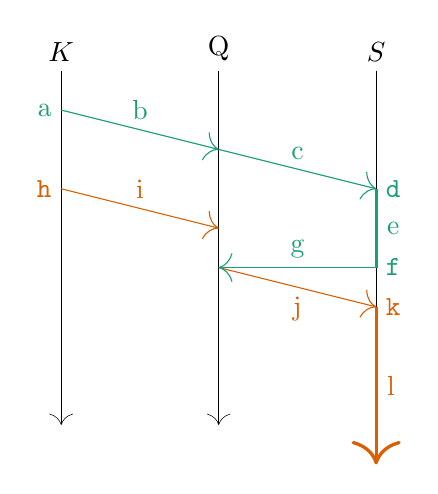
\begin{tikzpicture}
		\draw[very thin,-{>[scale=2]}] (0,10) -- (0,5.5) node[at start,anchor=south] {\(K\)};
		\draw[very thin,-{>[scale=2]}] (2,10) -- (2,5.5) node[at start, anchor=south] {Q};
		\draw[very thin] (4,10) -- (4,5) node[at start, anchor=south] {\(S\)};

		% from K
		\draw[-{>[scale=2]},dark2-1] (0,9.5) -- (2,9)
		node[at start,anchor=east] {a}
		node[midway,anchor=south] {b};
		\draw[-{>[scale=2]},dark2-2] (0,8.5) -- (2,8)
		node[at start,anchor=east] {\texttt{h}}
		node[midway,anchor=south] {i};

		% from Q
		\draw[-{>[scale=2]},dark2-1] (2,9) -- (4,8.5)
		node[at end,anchor=west] {\texttt{d}}
		node[midway,anchor=south] {c};
		\draw[-{>[scale=2]},dark2-2] (2,7.5) -- (4,7)
		node[at end,anchor=west] {\texttt{k}}
		node[midway,anchor=north] {j};

		% from S
		\draw[very thick,dark2-1] (4,8.5) -- (4,7.5)
		node[midway,anchor=west] {e};
		\draw[-{>[scale=2]},dark2-1] (4,7.5) -- (2,7.5)
		node[at start,anchor=west] {\texttt{f}}
		node[midway,anchor=south] {g};
		\draw[-{>[scale=2]},very thick,dark2-2] (4,7) -- (4,5)
		node[midway,anchor=west] {l};
	\end{tikzpicture}
	\caption{\label{fig:counterex}A simple failure example to demonstrate a race condition in the model.}
\end{figure}

\subsubsection{Model Solutions}

A client-side solution exists in forcing resolution of distributed object
references prior to sending any messages to the chunk queues.
This guarantees that any information relating to chunk alignment is cached with
each chunk reference, and that the server will always have access to this
information.
This would be immediately implementable, but will have a significant
corresponding drawback in removing prior asynchrony on the client end, blocking
a \mintinline{r}{do.call.distObjRef} until full chunk resolution of the
underlying arguments.
It is therefore not a full solution in itself, but removes race conditions
until a more complete solution is implemented.

The node acting as server presents a more likely candidate for the location of
a solution to the race condition.
If the \mintinline{r}{do.call.msg} was made concurrent through a
backgrounding-like operation, the blocking until alignment data was available
would remain, but with a guarantee of eventual availability of the data, thus
allowing for termination.

\subsubsection{Solution Implementation}

Implementation of server-side concurrency in the
\mintinline{r}{do.call.msg} and it's surrounding constructs implies a
parallel operation such as that provided by the \texttt{parallel} package,
located principally in the \mintinline{r}{mcparallel} function.
An initial problem with reliance on \mintinline{r}{mcparallel} is the
fork produces copy-on-write semantics, and so storing chunks in the local chunk
table becomes impossible when the chunk table is forked.
This may be overcome by removing the concept of a local chunk table, and
storing all objects in the local \texttt{osrv} server, which, being a separate
process, would not be forked itself. 
A potential problem in this solution is in the memory management of
\texttt{osrv}, and what would be done if references to the R objects are forked
away, but the data is intended to remain on the server.

\chapter{Platform User Interface}
\pkg{largescaler} serves as a functioning system, capable of performing complex statistical analyses over datasets spanning many nodes.
The implementation of this system makes use of a layered approach, wherein each layer targets a different category of user.
The \pkg{largescaler} interface is the principal new contribution by this project, delivering a novel means of interacting with distributed data through meaningful primitives defined at every level of abstraction.
A key offering of the layered approach is the ease by which a user of the package can traverse the levels as needed, with irrelevant information remaining hidden until required.
The levels of abstraction correspond to users of the package, given as the following:

\begin{description}
    \item[Analyst] A user solely interested in using the provided models and statistical functions in order to attain insight into some larger-than-memory data, typically a distributed data frame. All details of distribution are abstracted away.
    \item[Researcher] A user seeking to develop their own distributed statistical models. Distributed objects are to be considered as singular cohesive objects.
    \item[Developer] A user seeking greater expressivity in the definition of statistical models. Chunks are considered a relevant concern to be manipulated directly.
    \item[Architect] A user intending to directly modify the network topology of the distributed system, mainly in order to attain major efficiency gains.
\end{description}

Each of the users are served by the aforementioned packages making up the framework, in turn serving a logical layer of abstraction.
This mapping is given in Table \ref{tab:layer}.

\begin{table}[h!]
\centering
\caption{A mapping of logical layers, users and the respective packages provided by the \pkg{largescaler} framework to enable the use.}
\label{tab:layer}
\begin{tabular}{@{}lll@{}}
\toprule
Layer & User & Package \\ \midrule
Model Usage & Analyst & \pkg{largescalemodelr} \\
Model Description & Researcher & \pkg{largescaler} \\
Cluster Interaction & Developer & \pkg{chunknet} \\
Communication & Architect & \pkg{orcv} \\ \bottomrule
\end{tabular}
\end{table}

Owing to considerations of space, this description of the user interface will focus solely on the key offerings of the \pkg{largescaler} user interface, with descriptions of other components and packages having a fuller treatment in \cite{cairns2023}.
Use of the API is given by way of example below.

Consider first a simple operation of summation.
Given some vector $x$ that is broken up into $j$ chunks, yielding $j$ subvectors of length $i$.
Due to associativity the sum of the whole is the sum of the sum of the parts, as shown in Equation \ref{eqn:sum}.

\begin{equation}\label{eqn:sum}
    \sum_i x_i= \sum_{j,i}x_{ij} = \sum_j\sum_i x_{ij}
\end{equation}

In an effort to maintain as close proximity as possible between the mathematical description and the provided interface, this may be written in \pkg{largescaler} as in the following \proglang{R} code:

\code{ d(sum)(x) |> emerge() |> sum() }

Here, the \code{d()} applicator function transforms the base \code{sum()} function to work over distributed objects, in this example given by \code{x}.
\code{sum()} is therefore sent to each chunk, yielding a new distributed object as the output.
This output distributed object can be brought back to the requesting client and combined using the provided \code{emerge()} function, yielding a regular \proglang{R} numeric vector of sums.
This vector of sums may then be summed as normal, providing the final result.
The given example is actually a very simple application of map-reduce, and could effectively serve as the \code{sum()} method for distributed objects

Consider something slightly more complex: the arithmetic mean.
Again, a chunked mathematical description is given in Equation \ref{eqn:mean}

\begin{equation}\label{eqn:mean}
    \overline{x} = \frac{\sum_{i}x_{i}}{n} = \frac{\sum_{j,i}x_{ij}}{\sum_j n_j}
\end{equation}

A related means of specification through \pkg{largescaler} is possible, given in the following code:

\code{sum(x) / { d(length)(x) |> sum() } }

Here we build on the distributed sum introduced above, but the total length of The distributed object is relevent as the denominator.
Assuming a \code{sum()} method for distributed objects as described, and the math group generic defined in a similar fashion, the denominator is defined using the same \code{d()} function that sends a \code{length} computation to all of the chunks.

Finally, consider the cumulative sum.
It is important in this case to think of chunks as being in series, which is determined by the structure of the distributed object reference.
The main difference between a non-distributed and a distributed version of cumulative sum is that for each chunk in the series, computation requires the cumulative sum of the previous chunk as a starting value.
Using a chunked mathematical description, cumulative sum may be described by Equation \ref{eqn:cumsum}.

\begin{equation}
\begin{gathered}\label{eqn:cumsum}
    S_i = S_{i-1}+x_i, \quad S_0 = 0\\
    \iff S_{i,j} = S_{i-1,j} + x_{i,j}, \quad S_{0,j} = S_{n_i,j-1},\\
    \qquad S_{0,0} = 0
\end{gathered}
\end{equation}

This can be expressed in a functional manner using the \textit{reduce} operator, also known as a \textit{fold}, and the \pkg{largescaler} framework provides a distributed form of such a function, where the results of one chunk are sent as the initial value to the reduce function as applied to the next chunk and so on in series.
An example of a reduce operation is given in Figure \ref{fig:dreduce}.

\begin{figure}[ht]
\begin{center}
    \input{img/dreduce.tex}
\caption{Example distributed reduce pattern from controlling process.}
\label{fig:dreduce}
\end{center}
\end{figure}

This is put to use for cumulative sum by \pkg{largescaler} by the following code:

\code{ dReduce(cumsum, x) |> emerge() }

A distributed object is returned that by default just holds the final accumulation, consisting of one single chunk.
\chapter{User Interface Case Study: Distributed GLM}
With the interface for the final system laid down in \cref{ch:ui}, We now move to the central problem that prompted this work; defining a novel distributed statistical algorithm with it.
Rather than detour with a truly novel algorithm, it is prefereable to engage with something that is familiar, but holds a fairly generic form that novel analyses often share.
Let's consider distributed LASSO regression, using the Alternating Direction Method of Multipliers, as described by \textcite{mateos2010}.
We begin by assessing the mathematical form in \cref{sec:mathlasso}, followed by the ``standard R'' means of writing a chunked algorithm in contraposition with the \lsr{} manner in \cref{sec:rlasso}.

\section{Distributed LASSO Mathematical Definition}\label{sec:mathlasso}

This section seeks to give a brief taste of what a mathematical formulation for a distributed statistical model takes, in order to demonstrate the semantic and syntactic similarity to \lsr{} in \cref{sec:rlasso}.
A richer description, with significant background, is given in \textcite{boyd2011}.

We begin with a description of the input data, as given in \cref{eq:mathlassodata}

\eq{mathlassodata}

The starting data includes a column block matrix of explanatory variables, $A$, consisting of $N$ submatrices.
This is equivalent to a distributed object consisting of $N$ chunks.
Here, each chunk is of the standard form where rows are individual observations and columns are variables.
We also have a block matrix $b$ of the same number of chunks, with each chunk being the column vector of response variables to the corresponding $A$ chunks.

The standard form of the LASSO as an optimisation problem is expressed in \cref{eq:mathlassointention}.

\eq{mathlassointention}

The body of the ADMM loop is given by \cref{eq:mathlassoloop}.
Of note is the complexity, the presence of iteration, and the interactions between sets of chunks getting reduced and emerged.

\eq{mathlassoloop}

\section{Distributed LASSO R Description}\label{sec:rlasso}

This section gives both base \R{} syntax for working with a local chunked dataset, as well as the minimal changes that are required when using \lsr{} to transform the expressions to handle distributed data.
The core substance of this section is to demonstrate the ease with which \R{} is able to meet a mathematical definition, and the successive ease by which \lsr{} is able to turn that into a truly distributed algorithm.
As in \cref{sec:mathlasso}, the working example is given of distributed LASSO.
Consider first some chunked data, given as a diff in \cref{tab:chunked-comp}.
In the diff, semantic differences are demarcated through underlining, with shared code given centrally, with no dividing line.
On the left of the diff we have how the LASSO as described might be encoded in the absence of the API, assuming that the data fit into memory, and on the right, we make use of large scale \R{} with no such constraining assumption.

In the \lsr{} code, distributed data may come from multiple files and multiple hosts holding the chunks, and this is easily provided for.
The distribution comes with the necessity to carefully differentiate between the reference of the distributed object, and the distributed object itself.
The ability to explicitly distribute local values to particular locations is also demonstrated here.

\tab{chunked-comp}{Comparison of reading in chunks of data}

The layout of the data is followed by the iterative loop, given in \cref{tab:loop-comp}.
Within the iterative loop, we can see that very little is actually needed to be changed in order to distribute this algorithm.
We make use of a function that operates on distributed objects which we define ourselves in the successive diff, as well as the emerge to bring the distributed local as we saw before.

\tab{loop-comp}{Comparison of the iterative loop}

Note the significantly simplified and reduced logic in switching to \lsr{}, which bears a far closer resemblance to the mathematical description.
The \code{x-update} function given above is exemplary of the approach provided by \lsr{}, which allows for the switching of a local to a distributed function through the higher-order \code{dist} function, as demonstrated in \cref{tab:x-update}:

\tab{x-update}{Comparison of the \code{x-update} functions}

And this serves to define a distributed LASSO, using ADMM.

\chapter{Platform Implementation}
\chapter{Discussion on Delivered Platform}
\chapter{Conclusion}

\appendix
\chapter{Source Code}

\printbibliography

\end{document}